% This is samplepaper.tex, a sample chapter demonstrating the
% LLNCS macro package for Springer Computer Science proceedings;
% Version 2.20 of 2017/10/04
%
\newif\ifnotanonymous \notanonymousfalse
\newif\iffullversion \fullversiontrue
\documentclass[runningheads]{llncs}
%
\usepackage{graphicx}
\usepackage{color}
\usepackage{amsmath}
\usepackage{amssymb}
\usepackage{bcprules, proof}
\usepackage{fancybox}
\usepackage{mathtools}
\usepackage{float}
\usepackage{xparse}
\usepackage{lscape}
\usepackage{mdframed}
\usepackage{xspace}

% Used for displaying a sample figure. If possible, figure files should
% be included in EPS format.
%
% If you use the hyperref package, please uncomment the following line
% to display URLs in blue roman font according to Springer's eBook style:
% \renewcommand\UrlFont{\color{blue}\rmfamily}

\newcommand{\red}[1]{\textcolor{red}{#1 }}
\newcommand{\blue}[1]{\textcolor{blue}{#1 }}

\newcommand{\LTP}{$\lambda^{\triangleright\%}$\xspace}
\newcommand{\LMD}{$\lambda^{\textrm{MD}}$\xspace}
\newcommand{\LLF}{$\lambda\textrm{LF}$\xspace}

\newcommand{\G}{\Gamma}
\newcommand{\D}{\Delta}
\newcommand{\V}{\vdash_\Sigma}
\newcommand{\VT}{\vdash\hspace{-.50em}\raisebox{0.28em}{\tiny{$\TB$}}}
\newcommand{\iskind}{\text{\ kind}}
\newcommand{\TW}{{\mathop{\triangleright}}}
\newcommand{\TWL}{{\mathop{\triangleleft}}}
\newcommand{\F}{\forall}
\newcommand{\TB}{{\mathop{\blacktriangleright}}}
\newcommand{\TBL}{{\mathop{\blacktriangleleft}}}
\newcommand{\E}{\equiv}
\newcommand{\FV}{\text{FV}}
\newcommand{\FTV}{\text{FSV}}

\newcommand{\WStar}{\textsc{W-Star}}
\newcommand{\WAbs}{\textsc{W-Abs}}
\newcommand{\WCsp}{\textsc{W-Csp}}
\newcommand{\WApp}{\textsc{W-App}}
\newcommand{\WTW}{\textsc{W-$\TW$}}

\newcommand{\KVar}{\textsc{K-Var}}
\newcommand{\KAbs}{\textsc{K-Abs}}
\newcommand{\KApp}{\textsc{K-App}}
\newcommand{\KConv}{\textsc{K-Conv}}
\newcommand{\KTW}{\textsc{K-$\TW$}}
\newcommand{\KTWL}{\textsc{K-$\TWL$}}
\newcommand{\KGen}{\textsc{K-Gen}}
\newcommand{\KCsp}{\textsc{K-Csp}}

\newcommand{\TConst}{\textsc{T-Const}}
\newcommand{\TVar}{\textsc{T-Var}}
\newcommand{\TAbs}{\textsc{T-Abs}}
\newcommand{\TApp}{\textsc{T-App}}
\newcommand{\TConv}{\textsc{T-Conv}}
\newcommand{\TTB}{\textsc{T-$\TB$}}
\newcommand{\TTBL}{\textsc{T-$\TBL$}}
\newcommand{\TGen}{\textsc{T-Gen}}
\newcommand{\TIns}{\textsc{T-Ins}}
\newcommand{\TCsp}{\textsc{T-Csp}}

\newcommand{\QKAbs}{\textsc{QK-Abs}}
\newcommand{\QKCsp}{\textsc{QK-Csp}}
\newcommand{\QKRefl}{\textsc{QK-Refl}}
\newcommand{\QKSym}{\textsc{QK-Sym}}
\newcommand{\QKTrans}{\textsc{QK-Trans}}

\newcommand{\QTAbs}{\textsc{QT-Abs}}
\newcommand{\QTApp}{\textsc{QT-App}}
\newcommand{\QTTW}{\textsc{QT-$\TW$}}
\newcommand{\QTGen}{\textsc{QT-Gen}}
\newcommand{\QTCsp}{\textsc{QT-Csp}}
\newcommand{\QTRefl}{\textsc{QT-Refl}}
\newcommand{\QTSym}{\textsc{QT-Sym}}
\newcommand{\QTTrans}{\textsc{QT-Trans}}

\newcommand{\QAbs}{\textsc{Q-Abs}}
\newcommand{\QApp}{\textsc{Q-App}}
\newcommand{\QTB}{\textsc{Q-$\TB$}}
\newcommand{\QTBL}{\textsc{Q-$\TBL$}}
\newcommand{\QGen}{\textsc{Q-Gen}}
\newcommand{\QIns}{\textsc{Q-Ins}}
\newcommand{\QCsp}{\textsc{Q-Csp}}
\newcommand{\QRefl}{\textsc{Q-Refl}}
\newcommand{\QSym}{\textsc{Q-Sym}}
\newcommand{\QTrans}{\textsc{Q-Trans}}
\newcommand{\QBeta}{\textsc{Q-$\beta$}}
\newcommand{\QEta}{\textsc{Q-$\eta$}}
\newcommand{\QTBLTB}{\textsc{Q-$\TBL\TB$}}
\newcommand{\QLambda}{\textsc{Q-$\Lambda$}}
\newcommand{\QPercent}{\textsc{Q-\%}}

\newcommand{\ID}[1]{\infer[]{#1}{\vdots}}
\newcommand{\MD}[1]{\mathcal{D}_#1}

\newcommand{\I}{\textrm{Int}}
\newcommand{\B}{\textrm{Bool}}
\newcommand{\M}{\textrm{Mat}}
\newcommand{\Vpn}{\text{Vector}\ (\%_\alpha n)}

\newcommand{\AI}[1]{\textcolor{red}{[#1 -- AI]}}

\begin{document}
%
\title{A Dependently Typed Multi-Stage Calculus%
	\ifnotanonymous\thanks{Supported by organization x.}\fi
}
%
%\titlerunning{Abbreviated paper title}
% If the paper title is too long for the running head, you can set
% an abbreviated paper title here
%
\ifnotanonymous
	\author{Akira Kawata\inst{1} \and
		Atsushi Igarashi\inst{2}\orcidID{0000-0002-5143-9764}}
	% %
	\authorrunning{A. Kawata, A. Igarashi}
	% % First names are abbreviated in the running head.
	% % If there are more than two authors, 'et al.' is used.
	% %
	\institute{Graduate School of Informatics, Kyoto University, Kyoto, Japan\\
		\email{akira@fos.kuis.kyoto-u.ac.jp} \and
		\email{igarashi@kuis.kyoto-u.ac.jp}
	}
\fi
%
\maketitle              % typeset the header of the contribution
%
\begin{abstract}

	We study a dependently typed extension of a multi-stage programming
	language \`a la MetaOCaml, which supports quasi-quotation and
	cross-stage persistence for manipulation of code fragments as
	first-class values and eval for execution of programs dynamically
	generated by the code manipulation.  Dependent types are expected to
	bring to multi-stage programming enforcement of strong
	invariants---beyond simple type safety---on the behavior of
	dynamically generated code.  An extension is, however, not trivial
	because a type system would have to take stages---roughly speaking,
	the number of surrounding quotations---of types into account.
	
	To rigorously study properties of such an extension, we develop
	\LMD, which is an extension of Hanada and Igarashi's typed calculus
	\LTP with dependent types, and prove its properties including
	preservation, confluence, strong normalization for full
	reduction, and progress for staged reduction.  Motivated
	by code generators such that the type of generated code depends on a
	value from outside of quotations, we argue the significance of
	cross-stage persistence in dependently typed multi-stage programming
	and certain type equivalence that are not directly derived from
	reduction rules.
	
	% A multi-stage calculus enables us to generate and execute codes at runtime.
	% It can improve the performance of programs by generating optimized codes for given inputs.
	% Dependent types are types dependent on values. 
	% A vector with its length is a famous example of dependent types and it enables us to omit boundary checking.
	% In this paper, we design \LMD by introducing dependent type into $\lambda^{\TW\%}$.
	% You can make more efficient programs from existing dependent typed programs with \LMD.
	% \LMD has a simple, substitution-based full-reduction semantics and enjoys basic properties of subject reduction, confluence, and strong normalization, and progress.
	% It also includes an evaluation context which satisfies unique decomposition.
	% The main technical points of this paper are how to deal with Cross Stage Persistence of multi-stage calculuses which allows using a value in quoted code in a dependent type system.
	% Especially, the way of handling CSP in equivalence rules of dependent types wasn't clear.
	% In this paper, we give reasonable equivalence rules to handle them.
	
	\keywords{multi-stage programming, cross-stage persistence, dependent types}
\end{abstract}

\blue{181 words. The abstract should briefly summarize the contents of the paper in 150--250 words.}
\blue{コードとかはボールドを使ったほうが良いかもしれない。}
\red{Suspicious senetences are colored red.}
%
%
%
\red{Multi-stage Programming と Multi-stage Calculus をどう使い分けるか?}

% !TEX root = ../main.tex

\section{Introduction}

\subsection{Multi-stage Programming and MetaOCaml}

% \subsubsection{多段階計算とは何か?}

\AI{前の版は,まだ MetaOCaml specific な話と,MSP 一般の話が交互に出てきて
わかりづらかったと思います.}

Multi-stage programming makes it easier for programmers to implement
generation and execution of code at run time by providing language
constructs for composing and running pieces of code as first-class
values.  A promising application of multi-stage programming is
(run-time) code specialization, which is to generate program code
specialized to partial inputs to the program and such applications are
studied in the literature~\cite{taha2007gentle}  \AI{We should list
applications of multi-stage programming, not necessarily of MetaOCaml.}

MetaOCaml~\cite{calcagno2003implementing,oleg2014} is an extension of
OCaml\footnote{\url{http://ocaml.org}} with constructs for multi-stage
programming, including brackets, escape, run, and cross-stage
persistence (CSP) .  Brackets, written \verb|.< e >.| in MetaOCaml,
makes a value that represents the code (or abstract syntax tree) of
expression \verb|e|; and escape, written \verb|.~ e| and is supposed
to appear inside brackets, evaluates \verb|e| to a code value and
expands the code into the surrounding code.
For example,
\begin{verbatim}
   let plusone = .< fun x -> x + 1 >. in .< .~plusone 2 >.
\end{verbatim}
evaluates to \verb|.< (fun x -> x + 1) 2 >.|.  
Run, written \verb|run e|, evaluates \verb|e| to a code value
and executes it.  For example,
\begin{verbatim}
   run (let plusone = .< fun x -> x + 1 >. in .< .~plusone 2 >.)
\end{verbatim}
yields \verb|3| (here, escape connects tighter than application).
Finally, CSP is a primitive to embed values (not necessarily code
values) into a code value.  In MetaOCaml, CSP is implicitly applied to
occurrences of variables defined outside brackets.  For example,
\begin{verbatim}
   let plusone = fun x -> x + 1 in
   let y = plusone 2 in  .< y * 2 >.
\end{verbatim}
evaluates to \verb|.< 3 * 2 >.|, not \verb|.< plusone 2 * 2 >.|.
This is because the variable \verb|y| is bound to an integer \verb|3|
before \verb|.<y>.| is evaluated and the value of \verb|y| is embedded
into the code value.  In MetaOCaml, CSP can be applied to (variables of) any type.  CSP is practically important because it enables us to use library functions in brackets, e.g., \verb|.<List.combine [1;2] ['a';'b']>.|.

% \subsubsection{多段階計算のメリットをべき乗の例を用いて説明する}

% As we mentioned earlier, a main application of multi-stage
% calculi is program optimization. 
% A famous example is power functions.
% Usual power functions take two arguments, which are the base and the exponent.
% We can make a specialized power function for given exponents with multi-stage programming and 
% optimize them by unrolling a loop in functions for given exponents.
% The optimized power function for the exponent of \verb|3| looks like \verb|power3 = fun x -> x * x * x|.
% \verb|power3| is faster than ordinary \verb|power| function because it contains no loop.
% Multi-stage programming can optimize functions which take more than two arguments 
% by generating a code fragment optimized to a given argument.

% 多段階計算の型理論の既存研究の紹介

MetaOCaml is also equipped with a type system for safe code generation
and execution.  The notion of code types is introduced to prevent code
values that represent ill-typed expressions from being generated.  For
example,
\begin{verbatim}
   let plusone = .< fun x -> x + 1 >. in .< .~plusone "foo" >.
\end{verbatim}
is rejected by the MetaOCaml typechecker as \verb|plusone| is given
type \verb|(int -> int)| \verb|code| but it is used in the code context that
requires a function from \verb|string| is expected.  Ensuring safety
for \verb|run| is more challenging because basic code types do not
guarantee code values to be closed.  Taha and
Nielsen~\cite{taha2003environment} introduced the notion of
environment classifiers to address the problem and developed a type
system to ensure not only type-safe composition but also type-safe
execution of code values with a type soundness theorem.

However, the type system, which is based on Hindley--Milner
polymorphism~\cite{}, is not strong enough to guarantee invariants
beyond simple types.  For example, Kiselyov~\cite{} demonstrates
specialization of vector/matrix computation with respect to the sizes
of vectors and matrices but such specialized functions can be applied
to vectors and matrices of different sizes.

% Multi-stage programming can also optimize vector calculation.
% For example, \verb|vadd| function, which takes two vectors and return the sum of them,
% is implemented with a loop in many cases.
% We can unroll \verb|vadd| function for a given vector length and optimize it with multi-stage programming.

% % 多段階計算で生成したコードは特殊化されているが故に問題も多い

% However, there is a sever problem in functions which are optimized by multi-stage programming.
% Although unrolled \verb|vadd| function is optimized, we cannot use it for different vector length.
% For example, when you optimize for the length of 5, you shouldn't use it for vectors of 3 lengths.
% Otherwise, we will get a exception.
% This problem is serious but existing type systems for multi-stage calculi cannot prevent it.

\subsection{Multi-stage Programming with Dependent Types}

% 依存型とは何か?

One natural idea to address this problem is the introduction of dependent types
to express the size of data structure in static types~\cite{Xi98}.
% Dependent types are types which are dependent on values.
% We can use dependent types for securer programming like Xi and Pfenning
For example, we could declare vector types indexed by the size of
vectors as follows.
\begin{verbatim}
    Vector :: Int -> *
\end{verbatim}
\verb|Vector| is a type constructor that takes an integer (which
represents the length of vectors): for example, \verb|Vector 3| is the
type for vectors whose lengths are 3.  Then, our hope is to specialize
vector/matrix functions with respect to their size and get a piece of
function code, whose type respects the given size, \emph{provided at
  specilization time}.  For example, we would like to specialize a
function to add two vectors with respect to the size of vectors, that
is, to implement a code generator that takes an integer $n$ as an
input and generates a piece of function code of type
\verb|(Vector |$n$\verb| -> Vector|$n$\verb| -> Vector |$n$\verb|) code|.

% As we pointed out in the above section,
% functions optimized with multi-stage programming can take only restricted values as arguments.
% When you optimize \verb|vadd| function for the length of 5, you should it only for 5 length vectors.
% We introduce dependent types into a multi-stage calculus
% so that the type system can guarantee optimized functions are used properly.
% Although there is a trial to combine multi-stage programming and dependent type by Brady and Hammond~\cite{brady2006dependently},
% they didn't give a formal definition and properties for the calculus.

In this paper, we develop a new multi-stage calculus \LMD by extending
the existing multi-stage calculus \LTP\cite{Hanada2014}---which
formalizes the four constructs of MetaOCaml in a way slightly
different from MetaOCaml---with dependent types and study its
properties.  We base our work on \LTP because its type system and
semantics are arguably simpler than
\(\lambda^\alpha\)~\cite{taha2003environment}, which is more faithful
to the design of MetaOCaml.  Our technical contribution are summarized
as follows:
\begin{itemize}
\item We give the formal definition of \LMD with its syntax, 
  type system and two kinds of reduction---full and staged reduction.
\item We show preservation, strong normalization, and confluence for
  full reduction; and show unique decomposition (and progress as its
  corollary) for staged reduction, which formalizes program execution.
\end{itemize}
The combination of multi-stage programming and dependent types has
been discussed by Brady and Hammond~\cite{brady2006dependently} but,
to our knowledge, our work is a first formal calculus of dependently
typed multi-stage programming.

\subsection{Organization of the Paper}

The organization of this paper is as follows.
Section~\ref{sec:informal-overview} gives an informal overview of
\LMD.  Section~\ref{sec:formal-definition} defines \LMD and
Section~\ref{sec:properties} shows properties of \LMD.  Section
\ref{sec:related-work} discusses related work and Section
\ref{sec:conclusion} concludes the paper with discussion of future
work.


% !TEX root = ../main.tex

\section{Informal Overview of \LMD \label{sec:informal-overview}}

We describe our calculus \LMD informally.  \LMD is based on
\LTP~\cite{Hanada2014} by Hanada and Igarashi and so we start with a review of 
\LTP.

% \red{\LTP\cite{Hanada2014}が頻発するが同一論文の複数回引用に何かルールはあるのか?}
% \AI{ないです.たしかにあんまりつけるとうるさいですね.2.1 の冒頭とかは文ごと不要なのでは?}
\subsection{\LTP}

% quote and unquote

In \LTP, brackets (quasi-quotation) and escape (unquote) are written
$\TB_\alpha M$ and $\TBL_\alpha M$, respectively.  For example,
$\TB_\alpha (1 + 1)$ represents code of expression $1 + 1$ and thus
evaluates to itself.  Escape $\TBL_\alpha M$ may appear under
$\TB_\alpha$; it evaluates $M$ to a code value and splices it into the
surrounding code fragment.  Such splicing is expressed by the
following reduction rule:
\begin{align*}
	\TBL_\alpha (\TB_\alpha M) \longrightarrow M .
\end{align*}
% Using the type constructor $\TW_\alpha$ for code values, the type of
% $\TB_\alpha M$ is given $\TW_\alpha \tau$ if $M$ has type $\tau$; the type
% of $\TBL_\alpha M$ is $\tau$ if $M$ has $\TW_\alpha \tau$.

The subscript $\alpha$ in $\TB_\alpha$ and $\TBL_\alpha$ is a \textit{stage
  variable}\footnote{%
  In Hanada and Igarashi~\cite{Hanada2014}, it was called a
  \textit{transition variable}, which is derived from correspondence
  to modal logic, studied by Tsukada and Igarashi~\cite{Tsukada}.} and
a sequence of stage variables is called a \textit{stage}.  Intuitively,
they represent the depth of nested brackets.  Stage variables can be
abstracted by $\Lambda\alpha.M$ and instantiated by an application
$M\ A$ to stages.  For example,
$\Lambda\alpha.\TB_\alpha ((\lambda x:\I.x+10)\ 5)$ is a code value,
where \(\alpha\) is abstracted.  If it is applied to \(\alpha_1 \cdots \alpha_n\), \(\TB_\alpha\) becomes \(\TB_{\alpha_1} \cdots \TB_{\alpha_n}\); in particular,
if \(n = 0\), \(\TB_\alpha\) disappears.  So, an
application of $\Lambda\alpha.\TB_\alpha ((\lambda x:\I.x+10)\ 5)$
to the empty sequence \(\varepsilon\) reduces to
(unquoted) \((\lambda x:\I.x+10)\ 5\) and to 15.  In other words, application of
\(\Lambda\)-abstraction to $\varepsilon$ corresponds to \texttt{run}.
% If \(\alpha\) is instantiated with, say, \(\beta\gamma\), then
% \(\TB_\alpha\) becomes nested brackets \(\TB_{\beta} \TB_\gamma\).
This is expressed by the following reduction rule:
\begin{align*}
	(\Lambda\alpha.M)\ A \longrightarrow M[\alpha\mapsto A]
\end{align*}
where stage substitution \([\alpha \mapsto A]\) manipulates the nesting of
\(\TB_\alpha\) and \(\TBL_\alpha\) (and also \(\%_\alpha\) as we see later).

Cross-stage persistence (CSP), which is an important feature of \LTP,
is a primitive to embed values (not necessarily code values) into a
code value.  For example, a \LTP-term
\[
  M_1 = \lambda x:\I.\Lambda\alpha.(\TB_\alpha ((\%_\alpha x) * 2))
\]
takes an integer \(x\) as an input and returns a code value, into
which \(x\) is embedded.  If $M_1$ is applied to $38 + 4$ as in
\[
  M_2 = (\lambda x:\I.\Lambda\alpha.(\TB_\alpha ((\%_\alpha x) * 2)))\ (38 + 4),
\]
then it evaluates to
\(M_3 = \Lambda\alpha.(\TB_\alpha ((\%_\alpha 42) * 2))\).  According
to the semantics of \LTP, the subterm $\%_\alpha 42$ means that it
waits for the surrounding code to be run (by an application to
$\varepsilon$) and so it does not reduce further.  If \(M_3\) is run
by application to \(\varepsilon\), substitution of \(\varepsilon\) for
\(\alpha\) eliminates \(\TB_\alpha\) and \(\%_\alpha\) and so
\(42 * 2\), which reduces to 84, is obtained.
CSP is practically important because
one can call library functions from inside quotations.  

The type system of \LTP uses code types---the type of code of type
\(\tau\) is written \(\TW_\alpha \tau\)---for typing \(\TB_\alpha\),
\(\TBL_\alpha\) and \(\%_\alpha\).  It takes stages into account: a
variable declaration (written $x:\tau@A$) in a type environment is associated with its
declared stage $A$ as well as its type $\tau$ and the type judgement of \LTP is of
the form $\G \vdash M : \tau@A$, in which $A$ stands for the stage
of term $M$.\footnote{%
  In Hanada and Igarashi~\cite{Hanada2014}, it is written
  $\G \vdash^A M : \tau$.
  }
For example,
$y:\I@\alpha \vdash (\lambda x:\I.y) : \I \to \I @ \alpha$ holds, but
$y:\I@\alpha \vdash (\lambda x:\I.y) : \I \to \I @ \varepsilon$ does
not because the latter uses $y$ at stage \(\varepsilon\) but $y$ is
declared at $\alpha$.  Quotation \(\TB_\alpha M\) is given type
\(\TW_\alpha \tau\) at stage \(A\) if \(M\) is given type \(\tau\) at
stage \(A\alpha\); unquote \(\TBL_\alpha M\) is given type \(\tau\)
at stage \(A\alpha\) if \(M\) is given type \(\TW_\alpha \tau\) at
stage \(A\alpha\); and CSP \(\%_\alpha M\) is give type \(\tau\)
at stage \(A\alpha\) if \(M\) is given type \(\tau\) at \(A\).
These are expressed by the following typing rules.
\begin{center}
	\infrule{\G\vdash M:\tau @{A\alpha}}{\G\vdash \TB_{\alpha}M:\TW_{\alpha}\tau @A} \hfil
	\infrule{\G\vdash M:\TW_{\alpha}\tau @A}{\G\vdash \TBL_{\alpha}M:\tau @{A\alpha}} \hfil
	\infrule{\G\vdash M: \tau @A}{\G\vdash \%_{\alpha}M:\tau @{A\alpha}}
\end{center}
% \TTB, corresponding to brackets, means 
% if $M$ is typed $\tau$ at stage $A\alpha$ then $\TB_{\alpha}M$, quoted $M$, is typed $\TW_{\alpha}\tau$ at $A$.
% \TTBL\ is converse of \TTB.

% CSP


% Omitting Residualization
% この段落は3章のM eのあとに、この制限の結果として...という形で入れる

% There is another important feature called program residualization in \LTP.
% It means that a generated code can be dumped into a file.
% We can load the dumped file and run it.
% The difficulty arises when program residualization is used with CSP.
% Transition variables are classified into two kinds in \LTP in order to deal with this difficulty.

% \subsection{\LLF}

% % \LLF
% \LLF is a simple system of dependent types introduced in \cite{attapl}.
% It is made from Edinburgh LF\cite{harper1993framework} by omitting signatures and include declarative equality judgements.
% Hence, all constants and base types are declared in the signature.
% The \LLF type theory generalizes simply typed lambda calculus
% by replacing the function type $\tau\to\sigma$ with the dependent function type $\Pi x:\tau.\sigma$.

% % Kind, Well-formed kind
% In addition to ordinary typing rules like simply typed lambda calculus,
% there are kinding rules, well-formed kinding rules, term equivalence rules, type equivalence rules, and kind equivalence rules in \LLF.
% Kinding rules and well-formed kinding rules are 
% introduced in order to prohibit making illegal types such as $\textrm{Vector}\ \textrm{true}$.
% For a well-formed type $\tau$, $\G \vdash \tau :: K$ means that $\tau$ has a kind $K$ under the environment $\G$ and 
% for a well-formed kind $K$, $\G \vdash K$ means that $K$ is a well-formed kind under an environment $\G$.

% % Type Equality
% Type equality rules are needed because the type equivalence is not obvious unlike simply typed lambda calculus.
% For example, $\textrm{Vector}\ 7$ should be equivalent to $\textrm{Vector}\ (3+4)$
% but they are not equivalent seemingly. Thus, we must define equivalence rules.
% In \LLF, equivalence is expressed with a symbol of $\E$.
% $\G \vdash M \E N$ means a term $M$ and a term $N$ are equivalent under the environment $\G$.
% $\G \vdash \tau \E \sigma$ means a type $\tau$ and a type $\sigma$ are equivalent under the environment $\G$.
% $\G \vdash K \E J$ means a kind $K$ and a kind $J$ are equivalent under the environment $\G$.

\subsection{Extending \LTP with Dependent Types}

In this paper, we add a simple form of dependent types---{\`a} la
Edinburgh LF~\cite{harper1993framework} and \LLF~\cite{attapl}---to \LTP.
Types can be indexed by terms as in \texttt{Vector} in
Section~\ref{sec:intro} and \(\lambda\)-abstractions can be given
dependent function types of the form \(\Pi x:\tau. \sigma\) but we do
not consider type operators (such as $\texttt{list } \tau$) or
abstraction over type variables.  We introduce kinds to classify
well-formed types and equivalences for kinds, types, and terms---as
in other dependent type systems---but we have to address a question
how the notion of stage (should) interact with kinds and types.

On the one hand, base types such as \(\I\) should be able to be used
at every stage as in \LTP so that
\(\lambda x:\I.\Lambda \alpha. \TB_\alpha \lambda y:\I.M\) is a valid
term (here, \(\I\) is used at \(\varepsilon\) and \(\alpha\)).
Similarly for indexed types such as Vector 4.  On the other hand, it
is not clear how a type indexed by a variable, which can be used only
at a declared stage, can be used.  For example,
consider
\[\TB_\alpha (\lambda x:\I. (\TBL_\alpha (\lambda y:\text{Vector
  }x.M)N) )
  \text{ and }
  \lambda x:\I. \TB_\alpha (\lambda y:\text{Vector }x.M).
\]
Is Vector\ \(x\) a legitimate type at \(\varepsilon\) (and \(\alpha\),
resp.)  even if \(x:\I\) is declared at stage \(\alpha\) (and
\(\varepsilon\), resp.)?  We will give our answer to this question in two
steps.

First, type-level constants such as \(\I\) and Vector can be used at
every stage in \LMD.  Technically, we introduce a signature that
declares kinds of type-level constants and types of constants.  For
example, a signature for the Boolean type and constants is given as
follows $\B::*, \text{true}:\B, \text{false}:\B$ (where $*$ is the
kind of proper types).  Declarations in a signature are not
associated to particular stages; so they can be used at every stage.

Second, an indexed type such as Vector\ 3 or Vector\ $x$ is well
formed only at the stage(s) where the index term is well-typed.  Since
constant \(3\) is well-typed at every stage (if it is declared in the
signature), Vector\ 3 is a well-formed type at every stage, too.
However, Vector\ $M$ is well-formed only at the stage where index term
$M$ is typed.  Thus, the kinding judgment
of \LMD takes the form \(\G\V \tau :: K @ A\), where stage $A$ stands for
where \(\tau\) is well-formed.  For example,
given \(\text{Vector}:: \I \rightarrow *\) in the signature \(\Sigma\),
\(x:\I@\varepsilon \V \text{Vector }x :: * @\varepsilon\) can be
derived but
neither
\(x:\I@\alpha \V \text{Vector }x :: * @\varepsilon\)
nor 
\(x:\I@\varepsilon \V \text{Vector }x :: * @\alpha\)
can be.

At first, the restriction above sounds too severe, because a term like
\(\lambda x:\I. \TB_\alpha (\lambda y:\text{Vector }x.M) \), which models a
typical code generator which takes the size $x$ and returns code for vector
manipulation specialized to the given size, will be rejected. It seems crucial
for \(y\) to be given a type indexed by $x$. We can address this problem by
CSP---In fact, $\text{Vector }x$ is not well formed at $\alpha$ under
$x:\I@\varepsilon$ but $\text{Vector }(\%_\alpha x)$ is! So, we can still
write \(\lambda x:\I. \TB_\alpha (\lambda y:\text{Vector }(\%_\alpha x).M) \)
for the typical sort of code generators.

Our decision that well-formedness of types takes stages of index terms
into account will lead to the introduction of CSP at the type level
and special equivalence rules, as we will see later.


% !TEX root = ../main.tex

\section{Formal Definition of \LMD \label{sec:formal-definition}}
\label{sec:formal}

In this section, we give a formal definition of \LMD, including
the syntax, full reduction, and type system.  In addition to the full reduction,
in which any redex at any stage can be reduced, we also give staged reduction,
which models program execution (at \(\varepsilon\)-stage).

\subsection{Syntax}

We assume the denumerable set of \emph{type-level constants}, ranged over by
metavariables \(X, Y, Z\), the denumerable set of \emph{variables}, ranged
over by \(x,y,z\), the denumerable set of \emph{constants}, ranged over by
\(c\), and the denumerable set of \emph{stage variables}, ranged over by
\(\alpha, \beta, \gamma\).  The metavariables \(A, B, C\) range over
sequences of stage variables; we write \(\varepsilon\) for the empty
sequence. \LMD is defined by the following grammar:

{%\small
\begin{align*}
    % \textrm{Type variables}  &   &                          & X,Y,Z                                                                                                      \\
    % \textrm{Variables}       &   &                          & x,y,z                                                                                                      \\
    % \textrm{Stage variables} &   &                          & \alpha,\beta,\gamma                                                                                        \\
    % \textrm{Stage}           &   &                          & A,B,C                                                                                                      \\
    \textrm{kinds}             &  & K,J,I,H,G                & ::= * \mid \Pi x:\tau.K                                                           \\
    \textrm{types}             &  & \tau,\sigma,\rho,\pi,\xi & ::= X \mid \Pi x:\tau.\sigma \mid \tau\ M \mid \TW_{\alpha} \tau \mid \F\alpha.\tau \\
    %     \textrm{Constants}       &   &                          & c                                                                                                          \\
    \textrm{terms}             &  & M,N,L,O,P                & ::= c \mid x \mid \lambda x:\tau.M\ \mid M\ N \mid \TB_\alpha M                   \\
                               &  &                          & \ \ \ \ \mid \TBL_\alpha M \mid \Lambda\alpha.M \mid M\ A \mid \%_\alpha M        \\
    \textrm{signatures}         &  & \Sigma                   & ::= \emptyset \mid \Sigma, X::K \mid \Sigma, c:\tau                               \\
    \textrm{type env.} &  & \Gamma                   & ::= \emptyset \mid  \Gamma,x:\tau @A                                              \\
\end{align*}
}
% \AI{Add $M\,\alpha$ to terms.}

% \AI{Domain and FV are not defined (yet).  I think we should introduce the notion of well-formed type environments by prose below and assume every type environment is well formed.}

% Description of meta variables


% Kinds

A kind, which is used to classify types, is either $*$, the kind of
proper types (types that terms inhabit), or $\Pi x\colon\tau.K$, the kind
of type operators that takes $x$ as an argument of type $\tau$ and returns a type
of kind $K$.
% Types
% of terms have kind $*$ and dependent types have $\Pi$-kinds.  For
% example, $\lambda x:\I.x$ has type $\Pi x:\I.\I$, which has $*$ kind.
% \red{この段落は短いので型の段落と結合するか?}
% Types
A type is a type-level constant $X$, which is declared in the signature with its kind, a dependent function type $\Pi x:\tau.\sigma$,
an application $\tau\ M$ of a type (operator of $\Pi$-kind) to a term, a code type $\TW_\alpha \tau$, or an $\alpha$-closed type $\F\alpha.\tau$.
An example of an application of a type (operator) of $\Pi$-kind to a term is $\text{Vector}\ 10$; it is well kinded
if, say, the type-level constant $\text{Vector}$ has kind $\Pi x:\I.*$.
A code type $\TW_\alpha \tau$ is for a code fragment of a term of type $\tau$.
An $\alpha$-closed type, when used with $\TW_\alpha$, represents runnable code.

% An application $\tau\ M$ of a type (operator) to a term connects tighter than
% $\TW_{\alpha}$ connects tighter than
% $\Pi$ in dependent types such as $\Pi x:\tau.\tau$ and $\Pi$ connect tighter than
% $\F$ in types for stage abstraction such as $\F\alpha.\tau$.
% Therefore, $\F\alpha.\TW_{\alpha} \Pi x:\I.\text{Vector}\ 5$ is interpreted as
% $\F\alpha.(\TW_{\alpha} (\Pi x:\I.(\text{Vector}\ 5)))$.
% \AI{I don't understand this rule...}

% Terms

Terms include ordinary (explicitly typed) \(\lambda\)-terms, constants,
whose types are declared in signature $\Sigma$, and the following five forms
related to multi-stage programming:
$\TB_\alpha M$ represents a code fragment; $\TBL_\alpha M$ represents escape;
$\Lambda\alpha.M$ is a stage variable abstraction;
$M\ A$ is an application of a stage abstraction $M$ to stage $A$; and
$\%_\alpha M$ is an operator for cross-stage persistence.

% Signature

We adopt the tradition of \LLF-like systems, where types of constants and
kinds of type-level constants are globally declared in a signature $\Sigma$,
which is a sequence of declarations of the form $c:\tau$ and $X::K$. For
example, when we use Boolean in \LMD, $\Sigma$ includes $\B :: *,
\textrm{true}:\B, \textrm{false}:\B$. Type environments are sequences of
triples of a variable, its type, and its stage. We write
\(\textit{dom}(\Sigma)\) and \(\textit{dom}(\Gamma)\) for the set of
(type-level) constants and variables declared in \(\Sigma\) and \(\Gamma\),
respectively. As in other multi-stage
calculi~\cite{taha2003environment,Tsukada,Hanada2014}, a variable declaration
is associated with a stage so that a variable can be referenced only at the
declared stage. On the contrary, constants and type-level constants are
\emph{not} associated with stages; so, they can appear at any stage. We
define well-formed signatures and well-formed type environments later.

The variable $x$ is bound in $M$ by $\lambda x:\tau.M$ and in $\sigma$
by $\Pi x:\tau.\sigma$, as usual; the stage variable $\alpha$ is
bound in $M$ by $\Lambda \alpha.M$ and $\tau$ by $\F\alpha.\tau$.
The notion of free variables is defined in a standard manner.
We write $\FV(M)$ and $\FTV(M)$ for the set of free variables and the set of free stage variables in $M$, respectively.  Similarly, $\FV(\tau)$, $\FTV(\tau)$,
$\FV(K)$, and $\FTV(K)$ are defined.
We sometimes abbreviate $\Pi x:\tau_1.\tau_2$ to $\tau_1 \rightarrow \tau_2$ if
$x$ is not a free variable of $\tau_2$.
% Free variables
We identify $\alpha$-convertible terms and assume the names of bound variables are pairwise distinct.
% \AI{This should be mentioned after free variables are introduced.}
% \AI{What about other binders such as $\Pi$?}

The prefix operators $\TW_\alpha, \TB_\alpha, \TBL_\alpha$, and
$\%_\alpha$ are given higher precedence over the three forms $\tau\ M$, $M\ N$,
$M\ A$ of applications, which are left-associative. The binders $\Pi$,
$\forall$, and $\lambda$ extend as far to the right as possible.
Thus, $\F\alpha.\TW_{\alpha} (\Pi x:\I.\text{Vector}\ 5)$ is
interpreted as
$\F\alpha.(\TW_{\alpha} (\Pi x:\I.(\text{Vector}\ 5)))$; and
$\Lambda\alpha.\lambda x:\I.\TB_\alpha x\ y$ means
$\Lambda\alpha.(\lambda x:\I.(\TB_\alpha x)\ y)$.

\paragraph{Remark:} Basically, we define \LMD to be an extension of
\LTP with dependent types.  One notable difference is that \LMD has
only one kind of \(\alpha\)-closed types, whereas \LTP has two kinds
of \(\alpha\)-closed types \(\forall\alpha.\tau\) and
\(\forall^\varepsilon\alpha.\tau\).  We have omitted the first kind,
for simplicity, and dropped the superscript $\varepsilon$ from the second. It
would not be difficult to recover the distinction to show properties related
to program residualization~\cite{Hanada2014}, although they are left as 
conjectures.

\subsection{Reduction}

Next, we define full reduction for \LMD.
Before giving the definition of reduction, we define two kinds of substitutions.
Substitution $M[x\mapsto N], \tau[x \mapsto N]$ and $K[x \mapsto N]$ are
ordinary capture-avoiding substitution of
term $N$ for $x$ in term $M$, type $\tau$, and kind $K$, respectively,
and we omit their definitions here.
Substitution $M[\alpha \mapsto A], \tau [\alpha \mapsto A], K[\alpha \mapsto A]$ and $B[\alpha\mapsto A]$ are
substitutions of stage $A$ for stage variable $\alpha$ in term $M$, type $\tau$, kind $K$, and stage $B$, respectively.
We show representative cases below.
%
{%\small
\begin{align*}
    (\lambda x:\tau.M)[\alpha \mapsto A] & = \lambda x:(\tau[\alpha \mapsto A]).(M[\alpha \mapsto A])                                  \\
    (M\ B)[\alpha \mapsto A]             & = (M[\alpha \mapsto A])\ B[\alpha\mapsto A]                                                 \\
    (\TB_\beta M)[\alpha \mapsto A]      & = \TB_{\beta[\alpha \mapsto A]}M[\alpha \mapsto A]                                          \\
    (\TBL_\beta M)[\alpha \mapsto A]     & = \TBL_{\beta[\alpha \mapsto A]}M[\alpha \mapsto A]                                         \\
    (\%_\beta M)[\alpha \mapsto A]       & = \%_{\beta[\alpha \mapsto A]}M[\alpha \mapsto A]                                           \\
    (\beta B)[\alpha \mapsto A]          & = \beta (B[\alpha\mapsto A])                               & (\text{if } \alpha \neq \beta) \\
    (\beta B)[\alpha \mapsto A]          & = A (B[\alpha\mapsto A])                                   & (\text{if } \alpha = \beta)
\end{align*}
}
Here, $\TB_{\alpha_1\cdots\alpha_n} M$,
$\TBL_{\alpha_1\cdots\alpha_n} M$, and $\%_{\alpha_1\cdots\alpha_n} M$
$(n \geq 0)$ stand for $\TB_{\alpha_1} \cdots \TB_{\alpha_n} M$,
$\TBL_{\alpha_n}\cdots \TBL_{\alpha_1} M$, and
$\%_{\alpha_n}\cdots \%_{\alpha_1} M$, respectively.  
In particular,
$\TB_{\varepsilon} M = \TBL_{\varepsilon} M = \%_{\varepsilon} M = M$.
Also, it is important that
the order of stage variables is reversed for $\TBL$ and $\%$.
We also define substitutions of a stage or a term for variables in type environment $\G$.

\begin{definition}[Reduction]
    The relations $M \longrightarrow_\beta N$, $M \longrightarrow_\blacklozenge N$, and $M \longrightarrow_\Lambda N$
    are the least compatible relations closed under the rules below.
%    Congruence rules are omitted from the definition.
{%\small
    \begin{align*}
         (\lambda x:\tau.M) N & \longrightarrow_\beta M[x \mapsto N]         \\
         \TBL_\alpha \TB_\alpha M & \longrightarrow_\blacklozenge M          \\
         (\Lambda \alpha.M)\ A & \longrightarrow_\Lambda M[\alpha \mapsto A]
    \end{align*}
  }    
\end{definition}
We write $ M \longrightarrow M'$ iff $ M \longrightarrow_\beta M'$,
$ M \longrightarrow_\blacklozenge M'$, or
$ M \longrightarrow_\Lambda M'$ and we call $\longrightarrow_\beta$,
$\longrightarrow_\blacklozenge$, and $\longrightarrow_\Lambda$
$\beta$-reduction, $\blacklozenge$-reduction, and $\Lambda$-reduction,
respectively.
$M \longrightarrow^* N$ means that there is a sequence of reduction $\longrightarrow$ whose length is greater than or equal to 0.

The relation $\longrightarrow_\beta$ represents ordinary $\beta$-reduction in the \(\lambda\)-calculus; the relation
$\longrightarrow_\blacklozenge$ represents that quotation $\TB_\alpha M$ is canceled by escape and $M$ is spliced into the code fragment surrounding the escape;
the relation $\longrightarrow_\Lambda$ means that a stage abstraction applied to  stage $A$ reduces to the body of the abstraction
where $A$ is substituted for the stage variable.
There is no reduction rule for CSP as with Hanada and Igarashi \cite{Hanada2014}.
The CSP operator $\%_\alpha$ disappears when $\varepsilon$ is substituted for $\alpha$.
We show an example of a reduction sequence below.
Underlines show the redexes.
\begin{align*}
     & \hspace{10mm} \underline{(\lambda f:\I\to\I.(\Lambda\alpha.\TB_\alpha (\%_\alpha f\ 1 + (\TBL_\alpha \TB_\alpha 3))\ \varepsilon))\ (\lambda x:\I.x)} \\
     & \longrightarrow_\beta (\Lambda\alpha.\TB_\alpha (\%_\alpha (\lambda x:\I.x)\ 1 + (\underline{\TBL_\alpha \TB_\alpha 3})))\ \varepsilon        \\
     & \longrightarrow_\blacklozenge \underline{(\Lambda\alpha.\TB_\alpha (\%_\alpha (\lambda x:\I.x)\ 1 + 3))\ \varepsilon}                                         \\
     & \longrightarrow_\Lambda \underline{(\lambda x:\I.x)\ 1} + 3                                                                                           \\
     & \longrightarrow_\beta 1 + 3                                                                                                                           \\
     & \longrightarrow^* 4
\end{align*}

% $\TB_\alpha$ and $\TBL_\alpha$ disappears in the same way as $\%_\alpha$.

\subsection{Type System}

In this section, we define the type system of \LMD.
It consists of eight judgment forms for signature well-formedness, type environment well-formedness, kind well-formedness, kinding, typing, kind equivalence, type equivalence, and term equivalence.
We list the judgment forms in Figure~\ref{fig:LMD-six-judgments}.
They are all defined in a mutual recursive manner.  We will discuss
each judgment below.

\begin{figure}[tbp]
  \begin{center}
    \begin{align*}
      \vdash & \Sigma                     & \text{signature well-formedness}        \\
      \V     & \G                         & \text{type environment well-formedness} \\
      \G     & \V K \iskind @ A           & \text{kind well-formedness}             \\
      \G     & \V \tau :: K @ A           & \text{kinding}                          \\
      \G     & \V M : \tau @ A            & \text{typing}                           \\
      \G     & \V K \E J @ A              & \text{kind equivalence}                 \\
      \G     & \V \tau \E \sigma :: K @ A & \text{type equivalence}                 \\
      \G     & \V M \E N : \tau @ A       & \text{term equivalence}
    \end{align*}
    \caption{Eight judgment forms of the type system of \LMD.}
    \label{fig:LMD-six-judgments}
  \end{center}
\end{figure}


\subsubsection{Signature and Type Environment Well-formedness.}
The rules for Well-formed signatures and type environments are
shown below:
%
{\small
\begin{center}
  \infrule{
  }{
    \vdash \emptyset
  }
  \hfil
  \infrule{
    \vdash \Sigma \andalso
    \V K \iskind @ \varepsilon \\
    X\notin\textit{dom}(\Sigma)
  }{
    \vdash \Sigma, X::K
  }
  \hfil
  \infrule{
    \vdash \Sigma \andalso
    \V \tau :: * @ \varepsilon \\
    c\notin\textit{dom}(\Sigma)
  }{
    \vdash \Sigma, c:\tau
  }
  \\[2mm]
  \infrule{
  }{
    \V \emptyset
  }
  \hfil
  \infrule{
    \V \Gamma \andalso
    \Gamma \V \tau :: * @ A \andalso
    x\notin\textit{dom}(\Sigma)
  }{
    \V \Gamma, x:\tau@A
  }
\end{center}
}

To add declarations to a signature, the kind/type of a (type-level)
constant has to be well-formed at stage \(\varepsilon\) so that it is
used at any stage.  In what follows, well-formedness is not explicitly
mentioned but we assume that all signatures and type environments are
well-formed.

\subsubsection{Kind Well-formedness and Kinding.}

The rules for kind well-formedness and kinding are a straightforward
adaptation from \LLF and \LTP, except for the following rule for type-level CSP.
\begin{center}
  \infrule[K-Csp]{
    \G \V \tau :: * @ A
  }{
    \G \V \tau :: * @ A\alpha
  }
\end{center}
Unlike the term level, type-level CSP is implicit because there is no staged
semantics for types.

\subsubsection{Typing.}

\begin{figure}[tbp]
  \begin{center}
    \infrule[\TConst]{c:\tau \in \Sigma}{\G \V c:\tau @A} \hfil
    \infrule[\TVar]{x:\tau @A \in \G}{\G \V x:\tau @A} \\[2mm]
    \infrule[\TAbs]{\G\V \sigma::*@A\andalso\G,x:\sigma@A\V M:\tau @A}{\G\V(\lambda (x:\sigma).M):(\Pi (x:\sigma).\tau)@A} \\[2mm]
    \infrule[\TApp]{\G\V M:(\Pi (x:\sigma).\tau)@A \andalso \G\V N:\sigma@A}{\G\V M\ N : \tau[x\mapsto N]@A} \\[2mm]
    \infrule[\TConv]{\G\V M:\tau @A \andalso \G\V \tau\equiv \sigma :: K@A}{\G\V M:\sigma@A} \\[2mm]
    \infrule[\TTB]{\G\V M:\tau @{A\alpha}}{\G\V\TB_{\alpha}M:\TW_{\alpha}\tau @A} \andalso
    \infrule[\TTBL]{\G\V M:\TW_{\alpha}\tau @A}{\G\V\TBL_{\alpha}M:\tau @{A\alpha}} \\[2mm]
    \infrule[\TGen]{\G\V M:\tau @A \andalso \alpha\notin\rm{FTV}(\G)\cup\rm{FTV}(A)}{\G\V\Lambda\alpha.M:\forall\alpha.\tau @A} \\[2mm]
    \infrule[\TIns]{\G\V M:\forall\alpha.\tau @A}{\G\V M\ B:\tau[\alpha \mapsto B]@A} \andalso
    \infrule[\TCsp]{\G\V M:\tau @A}{\G\V \%_\alpha M:\tau @{A\alpha}}
    \caption{Typing Rules.}
    \label{fig:typing-rules}
  \end{center}
\end{figure}

The typing rules of \LMD are shown in Figure~\ref{fig:typing-rules}.
The rule \TConst{} means that a constant can appear at any stage.
% For example, if we have a signature $\Sigma$ which is
% $\textrm{bool} :: *, \textrm{true}: \textrm{bool}, \textrm{false}:
%     \textrm{bool}$, the derivation tree in
% Figure~\ref{fig:tconst-derivation-tree} is admissible.
The rules \TVar, \TAbs, and \TApp{} are almost the same as those in the simply typed
lambda calculus or \LLF.  Additional conditions are that subterms must be
typed at the same stage (\TAbs{} and \TApp); the type
annotation/declaration on a variable has to be a proper type of kind
$*$ (\TAbs) at the stage where it is declared (\TVar{} and \TAbs).
% \AI{Don't we need signature well formedness?  If $c:\tau \in \Sigma$, then $\tau$ should be a well-formed type under ... what?}
% \AI{... or \(\lambda\)LF?  We are working in a dependently type system...}  

% \begin{figure}
%     \begin{center}
%         \begin{minipage}{0.50\hsize}
%             \infer[\TConst]
%             {\G \V \textrm{true}:\textrm{bool}@\alpha\beta}
%             {\textrm{true}:\textrm{bool} \in \Sigma \andalso
%                 \ID{\G\V\textrm{bool}::*@\alpha\beta} \andalso
%             }
%             \caption{A derivation tree using \TConst}
%             \label{fig:tconst-derivation-tree}
%         \end{minipage}
%     \end{center}
% \end{figure}


% \TConv
As in standard dependent type systems, \TConv{} allows us to replace the type
of a term with an equivalent one. For example, assuming integers and
arithmetic, a value of type $\textrm{Vector}\ (4+1)$ can also have type
$\textrm{Vector}\ 5$ because of \TConv{}.

% Typing rules for a multi-stage calculus
The rules \TTB, \TTBL, \TGen, \TIns, and \TCsp{} are constructs for
multi-stage programming. \TTB{} and \TTBL{} are the same as in \LTP, as we
explained in Section \ref{sec:informal-overview}. The rule \TGen{} for stage
abstraction is straightforward. The condition
$\alpha\notin\rm{FTV}(\G)\cup\rm{FTV}(A)$ ensures that the scope of $\alpha$
is in $M$, and avoids capturing variables elsewhere. The
rule \TIns{} is for applications of stages to stage abstractions. The rule
\TCsp{} is for CSP, which means that, if term $M$ is of type $\tau$ at stage
$A$, then $\%_\alpha M$ is of type $\tau$ at stage $A\alpha$. Note that CSP
is also applied to the type \(\tau\) (although it is implicit) in the
conclusion. Thanks to implicit CSP, the typing rule is the same as in \LTP.


\subsubsection{Kind, Type and Term Equivalence.}

Since the syntax of kinds, types, and terms is mutually recursive,
the corresponding notions of equivalence are also mutually recursive.
They are congruences closed under a few axioms for term equivalence.
Thus, the rules for kind and type equivalences are not very interesting, 
except that implicit CSP is allowed.
We show a few representative rules below.

  {\small
    \begin{center}
      \infrule[\textsc{QK-Csp}]{%
        \G\V K \E J @ A
      }{
        \G\V K \E J @ A\alpha
      }
      \hfil
      \infrule[\QTCsp]{
        \G\V \tau \E \sigma :: *@A
      }{
        \G\V \tau \E \sigma :: *@{A\alpha}
      }
      \\[2mm]
      \infrule[\QTApp]{%
        \G\V \tau \E \sigma :: (\Pi x:\rho.K)@A \andalso
        \G\V M \E N : \rho @A
      }{
        \G\V \tau\ M \E \sigma\ N :: K[x \mapsto M]@A
      }
    \end{center}
  }

% The type equivalence judgment of the form
% $\G \V \tau \E \sigma : K @ A$ means that types $\tau$ and $\sigma$
% are equivalent as types of kind $K$ at stage $A$ under $\G$.
% Figure~\ref{fig:type-equivalence-rules} shows the rules for type
% equivalence.  Type equivalence is basically the least congruence
% closed under term equivalence.  The rules for compatibility (closure
% under type formation) are derived from corresponding typing rules in a
% straightforward manner.  The rules are a little simpler than some
% dependent type systems \AI{such as?}  because there is no abstraction
% at the type level.

% \QCsp以外の説明
% We show type equivalence rules in Figure \ref{fig:type-equivalence-rules}.
% All rules except \QTRefl, \QTSym, \QTTrans, and \QTApp\ are generated naturally from the typing rules.
% \QTRefl, \QTSym, \QTTrans\ exist in order to make the type equivalence relation an equivalence relationship.
% The rule \QTApp\ means that if there are two equivalent $\Pi$ type and two equivalent terms,
% the results of applications are also equivalent.

% \begin{figure}
%     \begin{center}
%         \infrule[{\QTAbs }]{\G\V \tau \E \sigma :: *@A \andalso \G,x:\tau @A \V \rho \E \pi :: *@A}{\G\V\Pi x:\tau.\rho \E \Pi x:\sigma.\pi :: *@A} \\[2mm]
%         \infrule[\QTApp]{\G\V \tau \E \sigma :: (\Pi x:\rho.K)@A \andalso \G\V M \E N : \rho @A}{\G\V \tau\ M \E \sigma\ N :: K[x \mapsto M]@A} \\[2mm]
%         \infrule[\textsc{QT-$\TW$}]{\G\V \tau \E \sigma :: *@{A\alpha}}{\G\V \TW_{\alpha} \tau \E \TW_{\alpha} \sigma :: *@A}\andalso
%         \infrule[\QTCsp]{\G\V \tau \E \sigma :: K@A}{\G\V \tau \E \sigma :: K@{A\alpha}} \\[2mm]
%         \infrule[\QTGen]{\G\V \tau \E \sigma :: *@A \andalso \alpha\notin\rm{FTV}(\G)\cup\rm{FTV}(A)}{\G\V \forall\alpha.\tau \E  \forall\alpha.\sigma :: *@A} \\[2mm]
%         \infrule[\QTRefl]{\G\V \tau::K@A}{\G\V \tau\E\tau :: K@A} \andalso
%         \infrule[\QTSym]{\G\V \tau \E \sigma :: K@A}{\G\V \sigma \E \tau :: K@A} \\[2mm]
%         \infrule[\QTTrans]{\G\V \tau \E \sigma :: K@A \andalso \G\V \sigma \E \rho  :: K@A}{\G\V \tau \E \rho  :: K@A}
%         \caption{Type Equivalence Rules.}
%         \label{fig:type-equivalence-rules}
%     \end{center}
% \end{figure}

% The term equivalence judgment of the form $\G \V M \E N : \rho @ A$,
% which means that terms $M$ and $N$ are equivalent as terms of type
% $\rho$ at stage $A$ under $\G$, is defined by the rules in
We show the rules for term equivalence  in
Figure~\ref{fig:term-equivalence-rules}, omitting
straightforward rules for reflexivity, symmetry, transitivity,
and compatibility.
% Most rules are
% straightforward.  The rules \QAbs, \QApp, \QTB, \QTBL, \QGen, \QIns,
% \QCsp, \QRefl, \QSym, and \QTrans{} make the relation congruence;
The rules \QBeta, \QTBLTB, and \QLambda{} correspond to
$\beta$-reduction, $\blacklozenge$-reduction, and $\Lambda$-reduction, respectively.

\begin{figure}[tbp]
  \begin{center}
    % \infrule[\QAbs]{\G\V \tau \E \sigma :: *@A \andalso \G,x:\tau @A \V M \E N : \rho @A}{\G\V\lambda x:\tau.M \E \lambda x:\sigma.N : (\Pi x:\tau.\rho)@A} \\[2mm]
    % \infrule[\QApp]{\G\V M \E L : (\Pi x:\sigma.\tau)@A \andalso \G\V N \E O : \sigma@A}{\G\V M\ N \E L\ O : \tau[x \mapsto N]@A} \\[2mm]
    % \infrule[\QTB]{\G\V M \E N : \tau @{A\alpha}}{\G\V \TB_\alpha M \E \TB_\alpha N : \TW_\alpha \tau @A} \andalso
    % \infrule[\QTBL]{\G\V M \E N : \TW_\alpha \tau @A}{\G\V \TBL_\alpha M \E \TBL_\alpha N : \tau @{A\alpha}} \\[2mm]
    % \infrule[\QGen]{\G\V M\E N : \tau @A \andalso \alpha \notin \FTV(\G)\cup\FTV(A)}{\G\V \Lambda\alpha.M \E \Lambda\alpha.N : \forall\alpha.\tau @A} \\[2mm]
    % \infrule[\QIns]{\G\V M \E N:\forall\alpha.\tau @A}{\G\V M\ \varepsilon \E N\ \varepsilon : \tau[\alpha \mapsto \varepsilon]@A} \andalso
    % \infrule[\QCsp]{\G\V M \E N : \tau @A}{\G\V\%_\alpha M \E \%_\alpha N : \tau @{A\alpha}} \\[2mm]
    % \infrule[\QRefl]{\G\V M:\tau @A}{\G\V M\E M : \tau @A} \andalso
    % \infrule[\QSym]{\G\V M\E N : \tau @A}{\G\V N\E M : \tau @A} \\[2mm]
    % \infrule[\QTrans]{\G\V M\E N : \tau @A \andalso \G\V N\E L : \tau @A}{\G\V M\E L : \tau @A} \\[2mm]
    \infrule[\QBeta]{\G,x:\sigma@A\V M:\tau @A \andalso \G\V N:\sigma@A}{\G\V(\lambda x:\sigma.M)\ N\E M[x\mapsto N] : \tau[x \mapsto N]@A} \\[2mm]
    % \infrule{\G\V M:(\Pi x:\sigma.\tau)@A \andalso x\notin \text{FV}(M)}{\G\V(\lambda x:\sigma.M\ x)\E M: (\Pi x:\sigma.\tau)@A}{\QEta} \\[2mm]
    \infrule[\QLambda]{\G\V (\Lambda\alpha.M) : \forall\alpha.\tau @A}{\G\V (\Lambda\alpha.M)\ \varepsilon \E M[\alpha \mapsto \varepsilon] : \tau[\alpha \mapsto \varepsilon]@A} \\[2mm]
    \infrule[\QTBLTB]{\G\V M \E N : \tau @A}{\G\V \TBL_\alpha(\TB_\alpha M) \E N : \tau @A} \hfil
    \infrule[\QPercent]{\G\V M:\tau @{A\alpha} \andalso \G\V M:\tau @A}{\G\V\%_\alpha M \E M : \tau @{A\alpha}}
    \caption{Term Equivalence Rules.}
    \label{fig:term-equivalence-rules}
  \end{center}
\end{figure}

% \QPercentの説明
The only rule that deserves elaboration is the last rule \QPercent.
Intuitively, it means that the CSP operator applied to term $M$ can be
removed if $M$ is also well-typed at the next stage \(A\alpha\).
For example, constants do not depend on the stage (see \TConst) and
so \(\G\V \%_\alpha c \E c : \tau @ A\alpha\) holds but variables
do depend on stages and so this rule does not apply.

\subsubsection{Example.}

We show an example of a dependently typed code generator in a
hypothetical language based on \LTP.  
% This rule is motivated by a practical consideration.
This language provides definitions by \textbf{let},
recursive functions (represented by \textbf{fix}), \textbf{if}-expressions,
and primitives cons, head, and tail to manipulate vectors. We assume that
$\text{cons}$ is of type $\Pi n:\I.\I \to \text{Vector}\ n \to \text{Vector}\ (n+1)$, 
$\text{head}$ is of type $\Pi n:\I.\text{Vector}\ (n+1) \to \I$, and
$\text{tail}$ is of type $\Pi n:\I.\text{Vector}\ (n+1) \to (\text{Vector}\ n)$.

Let's consider an application, for example, in computer graphics, in which we
have potentially many pairs of vectors of the fixed (but statically unknown)
length and a function---such as vector addition---to be applied to
them. This function should be fast because it is applied many times and be
safe because just one runtime error may ruin the whole long-running calculation.

% \AK{I strenghened this example by adding concrete situation. Do we need
% more reinforcements such as comparision with other method?} We will discuss
% the motivation through an example of specializing a vector addition function
% with respect to the size of vectors.

\newcommand{\Vpn}{\text{Vector}\ (\%_\alpha n)}

Our goal is to define the function vadd of type
\[
  \Pi n:\I.\F\beta.\TW_\beta(\Vpn\to\Vpn\to\Vpn).
\]
\renewcommand{\Vpn}{\text{Vector}\ n}
It takes the length $n$ and returns ($\beta$-closed) code of a
function to add two vectors of length $n$.  The generated
code is run by applying it to \(\varepsilon\) to obtain
a function of type \(\Vpn\to\Vpn\to\Vpn\) as expected.

We start with the helper function vadd$_1$, which takes a stage, the length $n$ of vectors, and two quoted vectors as arguments and returns code that computes the addition of the given two vectors:
%
\begin{tabbing}
	  $\textbf{let}\ \text{vadd}_1 : \F\alpha.\Pi n:\I.\TW_\alpha\Vpn\to\TW_\alpha\Vpn\to\TW_\alpha\Vpn$                                \\
	  \hspace{6mm} \= $= \textbf{fix}\ f.\Lambda\alpha.\lambda n:\I.\ \lambda v_1:\TW_\alpha\Vpn.\ \lambda v_2:\TW_\alpha\Vpn.$            \\
	  \> \hspace{6mm} \= $\textbf{if}\ n = 0 \ \textbf{then}\ \TB_\alpha \text{nil}$ \\
	  \>\> $\textbf{else}\ \TB_\alpha ($ \= $\textbf{let}\ t_1 = \text{tail}\ (\TBL_\alpha v_1)\ \textbf{in}$ \\
	  \>\>\> $\textbf{let}\ t_2 = \text{tail}\ (\TBL_\alpha v_2)\ \textbf{in}$ \\
          \>\>\> $\text{cons}\ $\= $(\text{head}\ (\TBL_\alpha v_1) + \text{head} \ (\TBL_\alpha v_2))$ \\
          \>\>\>\> $\TBL_\alpha (f\ (n-1)\ (\TB_\alpha t_1)\ (\TB_\alpha t_2)))$
\end{tabbing}
Note that the generated code will not contain branching on $n$ or recursion.
(Here, we assume that the type system can determine whether $n=0$ when
\textbf{then}- and \textbf{else}-branches are typechecked so that
both branches can be given type \(\TW_\alpha \text{Vector }n\).)

Using vadd$_1$, the main function vadd can be defined as follows:
\renewcommand{\Vpn}{\text{Vector}\ (\%_\beta n)}
\begin{align*}
	  & \textbf{let}\ \text{vadd}: \Pi n:\I.\F\beta.\TW_\beta(\Vpn\to\Vpn\to\Vpn)                \\ 
	  & \hspace{6mm} = \lambda n:\I.\Lambda\beta.\TB_\beta (\lambda v_1:\Vpn.\ \lambda v_2:\Vpn. \\
	  & \hspace{63mm} \TBL_\beta (\text{vadd}_1\ \beta\ n\ (\TB_\beta\ v_1)\ (\TB_\beta\ v_2))) 
\end{align*}
\renewcommand{\Vpn}{\text{Vector}\ (\%_\beta 5)}%
The auxiliary function vadd$_1$ generates code to compute addition of
the formal arguments $v_1$ and $v_2$ without branching on $n$ or recursion.
As we mentioned already, if this function is applied to a
(nonnegative) integer constant, say 5, it returns function code for adding
two vectors of size 5.  The type of vadd\ 5, obtained by
substituting 5 for $n$, is
$\F\beta.\TW_\beta(\Vpn\to\Vpn\to\Vpn)$.
\renewcommand{\Vpn}{\text{Vector}\ 5}
If the obtained code is run by applying to \(\varepsilon\),
the type of vadd\ 5\ $\varepsilon$ is
\(\Vpn\to\Vpn\to\Vpn\) as expected.

There are other ways to implement the vector addition function:
by using tuples instead of lists if the length
for all the vectors is statically known or by checking dynamically the
lengths of lists for every pair.  However, our method is better than
these alternatives in two points.  First, our function, $\text{vadd}_1$
can generate functions for vectors of arbitrary length unlike the one
using tuples.  Second, $\text{vadd}_1$ has an advantage in speed over
the one using dynamic checking because it can generate an optimized
function for a given length.

We make two technical remarks before proceeding:
\begin{enumerate}
\item If the generated function code is composed with another piece of code of type, say,
\(\TW_\gamma \text{Vector }5\), \QPercent{} plays an essential role; that is,
\(\text{Vector }5\) and \(\text{Vector }(\%_\gamma 5)\), which would occur
by applying the generated code to \(\gamma\) (instead of \(\varepsilon\)), are syntactically
different types but \QPercent{} enables to equate them.
Interestingly, Hanada and Igarashi~\cite{Hanada2014} rejected the idea of
reduction that removes $\%_\alpha$ when they developed \LTP{}, as such
reduction does not match the operational behavior of the CSP operator in
implementations. However, as an equational system for multi-stage programs,
the rule \QPercent{} makes sense.
\item \renewcommand{\Vpn}{\text{Vector}\ n}
By using implicit type-level CSP, the type of vadd
could have been written
\(\Pi n:\I.\F\beta.\TW_\beta(\Vpn\to\Vpn\to\Vpn)\).  In this type,
Vector\ $n$ is given kind at stage \(\varepsilon\) and type-level CSP
implicitly lifts it to stage \(\beta\).  However, if a type-level
constant takes two or more arguments from different stages, term-level
CSP is necessary.  A matrix type (indexed by the numbers of columns
and rows) would be such an example.
\end{enumerate}


\subsection{Staged Semantics}

The reduction given above is full reduction and any redexes---even
under $\TB_\alpha$---can be reduced in an arbitrary order.
Following previous work~\cite{Hanada2014},
we introduce (small-step, call-by-value) staged semantics,
where only $\beta$-reduction or $\Lambda$-reduction at stage $\varepsilon$ or the outer-most $\blacklozenge$-reduction are allowed,
modeling an implementation.

We start with the definition of values. Since terms under quotations are
not executed, the grammar is indexed by stages.

\begin{definition}[Values]
  The family $V^A$ of sets of values, ranged over by $v^A$,
  is defined by the following grammar.  In the grammar, $A' \neq \varepsilon$ is assumed.
  \begin{align*}
    v^\varepsilon \in V^\varepsilon & ::= \lambda x:\tau.M \mid\ \TB_\alpha v^\alpha \mid \Lambda\alpha.v^\varepsilon                                             & \\
    v^{A'} \in V^{A'}               & ::= x \mid \lambda x:\tau.v^{A'} \mid v^{A'}\ v^{A'} \mid\ \TB_\alpha v^{A'\alpha} \mid \Lambda\alpha.v^{A'} \mid v^{A'}\ B & \\
                                    & \quad\   \mid\ \TBL_\alpha v^{A''} (\text{if } A' = A''\alpha \text{ for some } \alpha, A'' \neq \varepsilon)               & \\
                                    & \quad\   \mid\ \%_\alpha v^{A''} (\text{if } A' = A''\alpha)
  \end{align*}
\end{definition}

Values at stage $\varepsilon$ are $\lambda$-abstractions, quoted pieces of code,
or $\Lambda$-abstractions.  The body of a $\lambda$-abstraction can
be any term but the body of $\Lambda$-abstraction has to be a value.  It
means that the body of $\Lambda$-abstraction must be evaluated.  The
side condition for $\TBL_\alpha v^{A'}$ means that escapes in a value
can appear only under nested quotations because an escape under a
single quotation will splice the code value into the surrounding
code.  See Hanada and Igarashi~\cite{Hanada2014} for details.

In order to define staged reduction, we define redex and evaluation contexts.

\begin{definition}[Redex]
  The sets of $\varepsilon$-redexes (ranged over by $R^\varepsilon$) and $\alpha$-redexes (ranged over by $R^\alpha$) are defined by the following grammar.
  \begin{align*}
     & R^\varepsilon ::= (\lambda x:\tau.M)\ v^\varepsilon \mid (\Lambda\alpha.v^\varepsilon)\ \varepsilon \\
     & R^\alpha      ::=\ \TBL_\alpha \TB_\alpha v^\alpha                                                         \\
  \end{align*}
\end{definition}

\begin{definition}[Evaluation Context]
  Let $B$ be either \(\varepsilon\) or a stage variable \(\beta\).
  The family of sets $ECtx^A_B$ of evaluation contexts, ranged over by $E^A_B$, is defined by the following grammar (in which $A'$ stands for a non-empty stage).
  %  $A$ is assumed to be nonempty (but $B,A'$ can be empty).
  \begin{align*}
    E^\varepsilon_B \in ECtx^\varepsilon_B & ::= \square\ (\text{if\ } B = \varepsilon)
    \mid E^\varepsilon_B\ M \mid v^\varepsilon\ E^\varepsilon_B \mid \TB_\alpha E^\alpha_B
    \mid \Lambda\alpha.E^\varepsilon_B \mid E^\varepsilon_B\ A                                                                                    \\
    E^{A'}_B \in ECtx^{A'}_B               & ::= \square\ (\text{if } A' = B) \mid \lambda x:\tau.E^{A'}_B \mid E^{A'}_B\ M \mid v^{A'}\ E^{A'}_B \\
                                           & \mid \TB_\alpha E^{A'\alpha}_B \mid \TBL_\alpha E^{A}_B \ (\text{where } A\alpha = A')               \\
                                           & \mid \Lambda\alpha.E^{A'}_B \mid E^{A'}_B\ A \mid \%_\alpha\ E^{A}_B \ (\text{where } A\alpha = A')
  \end{align*}
\end{definition}

The subscripts $A$ and $B$ in $E^A_B$ stand for the stage of the evaluation
context and of the hole, respectively. The grammar represents that staged
reduction is left-to-right and call-by-value and terms under \(\Lambda\) are
reduced. Terms at non-$\varepsilon$ stages are not reduced, except
redexes of the form \(\TBL_\alpha \TB_\alpha v^\alpha\) at stage \(\alpha\).
A few examples of
evaluation contexts are shown below:
\begin{align*}
  \square\ (\lambda x:\I.x)                  & \in  ECtx^\varepsilon_\varepsilon \\
  \Lambda\alpha.\square\ \varepsilon            & \in ECtx^\varepsilon_\varepsilon  \\
  \TBL_\alpha \TB_\alpha \TBL_\alpha \square & \in ECtx^\alpha_\varepsilon
\end{align*}
%
We write $E^A_B[M]$ for the term obtained by filling the hole $\square$ in $E^A_B$ by $M$.

Now we define staged reduction using the redex and evaluation contexts.

\begin{definition}[Staged Reduction]\sloppy
  The staged reduction relation, written $M \longrightarrow_s N$, is defined by
  the least relation closed under the rules below.
  \begin{align*}
    E^A_\varepsilon [(\lambda x:\tau.M)\ v^\varepsilon] & \longrightarrow_s E^A_\varepsilon[M[x\mapsto v^\varepsilon]]      \\
    E^A_\varepsilon [(\Lambda\alpha.v^\varepsilon)\ A]  & \longrightarrow_s E^A_\varepsilon[v^\varepsilon[\alpha\mapsto A]] \\
    E^A_\alpha [\TBL_\alpha \TB_\alpha v^\alpha]        & \longrightarrow_s E^A_\alpha[v^\alpha]                            \\
  \end{align*}
\end{definition}

This reduction relation reduces a term in a deterministic,
left-to-right, call-by-value manner.  An application of an abstraction
is executed only at stage \(\varepsilon\) and only a quotation at
stage \(\varepsilon\) is spliced into the surrounding code---notice
that, if \(\TB_\alpha v^\alpha\) is at stage \(\varepsilon\), then the
redex \(\TBL_\alpha \TB_\alpha v^\alpha\) is at stage \(\alpha\).
In other words, terms in brackets are not evaluated until the terms are run
and arguments of a function are evaluated before the application.
We show an example of staged reduction.
Underlines show the redexes.
\begin{align*}
                    & (\Lambda\alpha.(\TB_\alpha \underline{\TBL_\alpha \TB_\alpha ((\lambda x:\I.x)\ 10))})\ \varepsilon \\
  \longrightarrow_s & \underline{(\Lambda\alpha.(\TB_\alpha ((\lambda x:\I.x)\ 10)))\ \varepsilon}                        \\
  \longrightarrow_s & \underline{(\lambda x:\I.x)\ 10}                                                                    \\
  \longrightarrow_s & 10
\end{align*}


% !TEX root = ../main.tex

\section{Properties of \LMD \label{sec:properties}}

In this section, we show the basic properties of \LMD: preservation, strong
normalization, confluence for full reduction, and progress for staged
reduction.

% Substitution Lemma

The Substitution Lemma in \LMD{} is a little more complicated than usual
because there are eight judgment forms and two kinds of substitution.
The Term Substitution Lemma states that term substitution $[z \mapsto M]$
preserves derivability of judgments. The Stage Substitution Lemma
states similarly for stage substitution $[\alpha\mapsto A]$.

We let $\mathcal{J}$ stand for the judgments $K \iskind @A$, $\tau::K@A$,
$M:\tau@A$, $K \E J @ A$, $\tau \E \sigma @ A$, and
$M \E N : \tau @ A$.  Substitutions $\mathcal{J}[z \mapsto M]$ and
$\mathcal{J}[\alpha \mapsto A]$ are defined in a straightforward
manner.  Using these notations, the two substitution lemmas are stated as follows:

We proved the next two leammas by simultaneous induction on derivations.

\begin{lemma}[Term Substitution]
  If $\G, z:\xi@B, \D \V \mathcal{J}$ and $\G\V P:\xi @B$, then $\G, (\D[z \mapsto P]) \V \mathcal{J}[z \mapsto P]$.  Similarly, if $\V \G, z:\xi@B, \D$ and
  $\G\V P:\xi @B$, then $\V \G, (\D[z \mapsto P])$.
\end{lemma}

\begin{lemma}[Stage Substitution]
	If $\G \V \mathcal{J}$, then $\G[\beta\mapsto B] \V \mathcal{J}[\beta\mapsto B]$.  Similarly, if $\V \G$, then $\V \G[\beta\mapsto B]$.
\end{lemma}

% Inversion Lemma

The following Inversion Lemma is needed to prove the main theorems.
As usual~\cite{TAPL}, Inversion Lemma enables us to infer the types of subterms of a term from the type of the term.

\begin{lemma}[Inversion]\ 
	\begin{enumerate}
		\item If $\G \V (\lambda x:\sigma.M) : \rho$ then there are $\sigma'$ and $\tau'$ such that
		      $\rho = \Pi x:\sigma'.\tau'$, $\G \V \sigma \E \sigma'@A$ and $\G ,x:\sigma'@A\V M:\tau'@A$.
		\item If $\G \V \TB_\alpha M : \tau@A$ then 
		      there is $\sigma$ such that $\tau = \TW_\alpha \sigma$ and $\G \V M : \sigma@A$.
		  \item If $\G \V \Lambda\alpha.M : \tau$ then 
		  there is $\sigma$ such that $\sigma = \forall\alpha.\sigma$ and $\G \V M : \sigma@A$.% and $\alpha \notin \FTV(\G) \cup \FV(A)$.
	\end{enumerate}
\end{lemma}

\begin{proof}
  Each item is strengthened by statements about type equivalence.
  For example, the first statement is augmented by
  \begin{quotation}
    If $\G \V \rho \E (\Pi x:\sigma.\tau) : K @A$, then there exist
    $\sigma'$ and $\tau'$ such that $\rho = \Pi x:\sigma'.\tau'$ and
    $\G \V \sigma \E \sigma' : K @A$ and
    $\G, x:\sigma@A\V \tau \E \tau' : J @A$.
  \end{quotation}
  and its symmetric version.  Then, they are proved simultaneously by induction on derivations.
  Similarly for the others.
 \qed
\end{proof}


% Preservation

Thanks to Term/Stage Substitution and Inversion, we can prove Preservation easily.

\begin{theorem}[Preservation]
	If $\G\V M:\tau @A$ and $M \longrightarrow M'$, then $\G\V M':\tau @A$.
\end{theorem}

\begin{proof}
	First, there are three cases for $M \longrightarrow M'$.
	They are $M \longrightarrow_\beta M'$, $M \longrightarrow_\Lambda M'$, and $M \longrightarrow_\blacklozenge M'$.
	For each case, we can use straightforward induction on typing derivations.
	% Difficult cases are \TApp, \TTBL, and \TIns.
	% We need Inversion Lemmas for them.
\end{proof}

% Strong Normalization

Strong Normalization is also an important property, which guarantees that
no typed term has an infinite reduction sequence.
Following standard proofs (see, e.g., \cite{harper1993framework}), we prove this theorem by translating \LMD to the simply typed lambda calculus.

\begin{theorem}[Strong Normalization]
	If $\G\V M_1:\tau@A$ then there is no infinite sequence $(M_i)_{i\ge1}$ of terms such that
	$M_i \longrightarrow M_{i+1}$ for $i\ge 1$.
\end{theorem}

\begin{proof}
	In order to prove this theorem, we define a translation $(\cdot)^\natural$ from \LMD\ to the simply typed lambda calculus.
	Second, we prove the $\natural$-translation preserves typing and reduction.
	Then, we can prove Strong Normalization of \LMD from Strong Normalization of the simply typed lambda calculus.
\end{proof}

Confluence is a property that any reduction sequences from one typed term converge.
Since we have proved Strong Normalization, we can use Newman's Lemma~\cite{DBLP:books/daglib/0092409} to prove Confluence.

\begin{theorem}[Confluence]
	For any term $M$, if $M \longrightarrow^* M'$ and $M \longrightarrow^* M''$ then
	there exists $M'''$ that satisfies $M' \longrightarrow^* M'''$ and $M'' \longrightarrow^* M'''$.
\end{theorem}

\begin{proof}
  We can easily show Weak Church-Rosser.  Use Newman's Lemma.
	% Because we proved Strong Normalization of \LMD, 
	% we can use Newman's lemma to prove Confluence of \LMD.
	% Then, what we must show is Weak Church-Rosser Property now.
	% When we consider two different redexes in a \LMD term, they can only be disjoint, or one is a part of the other.
	% In short, they are never overlapped each other.
	% So, we can reduce one of them after we reduce another.
\end{proof}

Now, we turn our attention to staged semantics.  First, the staged
reduction relation is a subrelation of full reduction, so Subject
Reduction holds also for the staged reduction.

\begin{theorem}
  If $M \longrightarrow_s M'$, then $M \longrightarrow M'$.
\end{theorem}
\begin{proof}
  Easy.
 \qed
\end{proof}

The following theorem Unique Decomposition ensures that, every typed
term is either a value or can be uniquely decomposed to an evaluation
context and a redex, ensuring that a well-typed term is not
immediately stuck and the staged semantics is deterministic.

\begin{theorem}[Unique Decomposition]
  If $\G$ does not have any variable declared at stage $\varepsilon$ 
  and $\G \V M : \tau @ A$, then either
  \begin{enumerate}
  \item $ M \in V^A$, or
  \item $M$ can be uniquely decomposed into an evaluation context and a redex, that is, there uniquely exist $B, E^A_B$, and $R^B$ such that $M = E^A_B[R^B]$.
  \end{enumerate}
\end{theorem}

\begin{proof}
  We can prove by straightforward induction on typing derivations.
%  Main cases are \TApp, \TTBL, and \TIns, where we use Inversion.
  \qed
\end{proof}

The type environment $\G$ in the statement usually has to be empty;
in other words, the term has to be closed.  The condition is relaxed here
because variables at stages higher than \(\varepsilon\) are considered
symbols.  In fact, this relaxation is required for proof by induction
to work.

% This theorem is important because it guarantees
% that the evaluation context decides a redex to reduce deterministically.
% Specifically speaking, this theorem guarantee that 
% when you write a interpreter using the evaluation context of \LMD,
% your interpreter works just as intended.
      
Progress is a corollary of Unique Decomposition.

\begin{corollary}[Progress]
	If $\G$ does not have any variable declared at stage $\varepsilon$ and $\G \V M : \tau  @ A$, then
	$ M \in V^A $ or there exists $M'$ such that $M \longrightarrow_s M'$.
\end{corollary}



% !TEX root = ../main.tex

\section{Related Work}

% 多段階計算の歴史

Multi-stage calculi also have a long history of research.
Davis revealed there is Curry-Howard correspondence between a multi-stage calculus and modal logic in $\lambda^\circ$ \cite{davies1996temporal}.
However, $\lambda^\circ$ don't have operators for run and CSP.
Benaissa, et al. \cite{benaissa1999logical} study the relationship between multi-stage calculus and category theory or modal logic.
Taha and Sheard introduced run and CSP to a multi-stage calculus in \cite{MetaML}.
Additionally, Taha and Nielsen invented the concept of environment classifiers in $\lambda^\alpha$ \cite{taha2003environment} and 
construct the type system for $\lambda^\alpha$, which can handle quoting, unquoting, run, and CSP.

In $\lambda^\TW$ \cite{Tsukada}, Tsukada and Igarashi found modal logic which corresponds to a multi-stage calculus with environment classifiers and
show that run can be represented as application of $\varepsilon$ to transition abstractions.
In \LTP \cite{Hanada2014}, Hanada and Igarashi extended $\lambda^\TW$ with CSP and discuss code residualization 
which allows us to dump the quoted code into an external file.

% 他段階計算の機能拡張

Combination of multi-stage programming and another programming feature has been studied.
Oleg, Kameyama, and Sudo\cite{kiselyov2016refined} designed a type sysytem for multi-stage programming with mutable cells and
Oishi and Kameyama\cite{oishi2017staging} extended a multi-stage calculus so that it can handle control operators such as shift and reset.

% 多段階計算の応用

MetaOCaml is a programming language with quoting, unquoting, run, and CSP.
Oleg gave many examples of application of MetaOCaml in \cite{8384206}, 
which include filtering in signal processing, matrix-vector product, and DSL compiler.

% 依存型の歴史

There are many papers on dependent types and most of them are affected by the pioneering work of Per Martin-L\"{o}f \cite{martin1973intuitionstic}.
$\lambda^\Pi$ \cite{Meyer1986}, Calculus of Constructions \cite{coquand:inria-00076024}, 
and Harper, Honsell and Plotkin \cite{harper1993framework} are famous papers on dependent types.
In Advanced Topics in Types and Programming Languages \cite{attapl},
a dependent type system \LLF is designed with the basis of \cite{harper1993framework}.
We adopted \cite{attapl}-like dependent types for \LMD.

% 依存型の応用

Applications of dependent types for real problems were also researched.
One can use dependent types in programming languages such as Idris\cite{brady2013idris} or
interactive theorem provers such as Coq\cite{09thecoq} which based on \cite{coquand:inria-00076024}.
In Xi and Pfenning \cite{Xi98}, they extended SML with restricted dependent types
and succeeded in reducing the bounds checking of arrays.
In Xi and Robert \cite{xi2001dependently}, they design a type system for an assembly language and
it is useful for spped up.
Xi also gave dead code elimination and loop unrolling as examples of dependent types application in \cite{xi1999dependent}.

% 関連研究との比較

Brady and Hammond \cite{brady2006dependently} extended a dependent type system 
with Taha's staging technique \cite{taha2007gentle} in order to implement a staged interpreter.
However, they focused on implementation and there is no theoritical discussion in their paper.

% 他の方法としてどのようなものが考えられたか

Although we define type equivalence of \LMD with composition of equivalence rules,
there is another candiate to define,
which gives reduction on types and compare the results of reduction such as \cite{sorensen2006lectures}.
This method is better than one of \LMD because equivalence rules become simple.
However, we reject it because it cannot handle CSP flexibly.

% !TEX root = ../main.tex

\section{Conclusions}

We proposed new multi-stage calculus \LMD, which can use dependent types.
\LMD enable finer-grained typing of multi-stage programming comparing to existing type systems.
This extention prevent some bugs relating to generated functions with multi-stage programming,
such as \verb|vadd| function for vectors of a fixed length.
We proved properties of \LMD including preservation, confluence, 
strong normalization for full reduction, and progress for staged reduction.
The technical difficulty of extention is how to deal with the symbol of CSP $\%$ in the equation rules.
We resolve this problem by ignoring $\%$ under some condition.

Making algorithmic typing and equality rules for \LMD is a future work.
They would be complicated but possible 
because we can realize them by defining a new weak head normal form which contains $\%$ erasing rule.

% \begin{enumerate}
% 	\item Done: On Cross-Stage Persistence in Multi-Stage\cite{Hanada2014}
	      
% 	      CSPも入りました
% 	\item Done: Eliminating Array Bound Checking Through Dependent Types\cite{Xi98}
% 	\item Done: MetaML and Multi-stage Programming with Explicit Annotations\cite{MetaML}
% 	\item Done: Idris, a general-purpose dependently typed programming language: Design and implementation\cite{brady2013idris}
% 	\item Done: A Logical Foundation for Environment Classifiers\cite{Tsukada}
% 	\item Done: Environment classifiers\cite{taha2003environment}
% 	\item Done: A framework for defining logics\cite{harper1993framework}
	      
% 	      $\Sigma$ の使い方を確認した
% 	\item Done: The Design and Implementation of {BER} MetaOCaml - System Description\cite{oleg2014}
% 	\item Done: Dependent types in practical programming\cite{xi1999dependent}
	      
% 	      Section of Applicationを読んだ。Dead Code EliminationやLoop Unrollingにも使えるらしい。
	      
% 	\item Done: A dependently typed assembly language\cite{xi2001dependently}
	      
% 	      DTALの定義と制約solverを用いた型検査の定義
% 	\item Done: Refined Environment Classifiers\cite{kiselyov2016refined}
% 	\item Done: Staging with control: type-safe multi-stage programming with control operators\cite{oishi2017staging}
% 	\item Done: Logical Modalities and Multi-Stage Programming\cite{benaissa1999logical}
% 	\item \red{Partial evaluation and automatic program generation}\cite{jones1993partial}
% 	\item \red{Efficient multi-level generating extensions for program specialization}\cite{gluck1995efficient}
% 	\item \red{Run-time code generation and Modal-ML}\cite{wickline1998run}
% 	\item \red{C and tcc: a language and compiler for dynamic code generation}\cite{poletto1999c}
% 	\item \red{Run-time bytecode specialization}\cite{masuhara2001run}
% 	\item \red{A tour of Tempo: A program specializer for the C language}\cite{consel2004tour}
% 	\item \red{Optimizing ML with run-time code generation}\cite{lee1996optimizing}
% 	\item \red{Efficient incremental run-time specialization for free}\cite{marlet1999efficient}
% \end{enumerate}

% 2つの設計手法と今回採用した理由
% Conclusion送りか?
% When we design type equivalence rules of \LMD, there are two design choices.
% One is defining type equivalence by $\beta$-equality after we define $\beta$-reduction of types.
% Another is defining type equivalence directly by a combination of type equivalence rules.
% We adopt the latter one because it is convenient to handle CSP in the type equivalence.

% \section{First Section}
% \subsection{A Subsection Sample}
% Please note that the first paragraph of a section or subsection is
% not indented. The first paragraph that follows a table, figure,
% equation etc. does not need an indent, either.
% 
% Subsequent paragraphs, however, are indented.
% 
% \subsubsection{Sample Heading (Third Level)} Only two levels of
% headings should be numbered. Lower level headings remain unnumbered;
% they are formatted as run-in headings.
% 
% \paragraph{Sample Heading (Fourth Level)}
% The contribution should contain no more than four levels of
% headings. Table~\ref{tab1} gives a summary of all heading levels.
% 
% \begin{table}
% \caption{Table captions should be placed above the
% tables.}\label{tab1}
% \begin{tabular}{|l|l|l|}
% \hline
% Heading level &  Example & Font size and style\\
% \hline
% Title (centered) &  {\Large\bfseries Lecture Notes} & 14 point, bold\\
% 1st-level heading &  {\large\bfseries 1 Introduction} & 12 point, bold\\
% 2nd-level heading & {\bfseries 2.1 Printing Area} & 10 point, bold\\
% 3rd-level heading & {\bfseries Run-in Heading in Bold.} Text follows & 10 point, bold\\
% 4th-level heading & {\itshape Lowest Level Heading.} Text follows & 10 point, italic\\
% \hline
% \end{tabular}
% \end{table}
% 
% 
% \noindent Displayed equations are centered and set on a separate
% line.
% \begin{equation}
% x + y = z
% \end{equation}
% Please try to avoid rasterized images for line-art diagrams and
% schemas. Whenever possible, use vector graphics instead (see
% Fig.~\ref{fig1}).
% 
% \begin{figure}
% 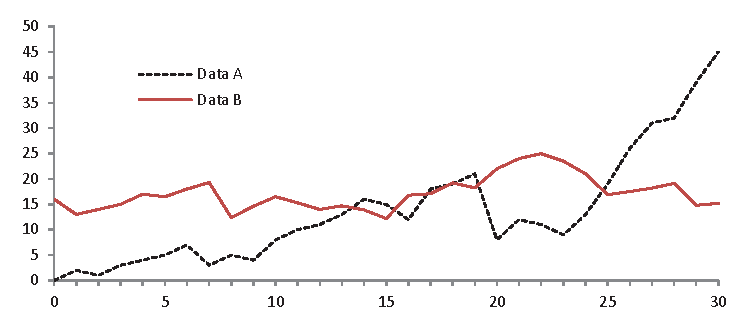
\includegraphics[width=\textwidth]{fig1.eps}
% \caption{A figure caption is always placed below the illustration.
% Please note that short captions are centered, while long ones are
% justified by the macro package automatically.} \label{fig1}
% \end{figure}
% 
% \begin{theorem}
% This is a sample theorem. The run-in heading is set in bold, while
% the following text appears in italics. Definitions, lemmas,
% propositions, and corollaries are styled the same way.
% \end{theorem}
% %
% % the environments 'definition', 'lemma', 'proposition', 'corollary',
% % 'remark', and 'example' are defined in the LLNCS documentclass as well.
% %
% \begin{proof}
% Proofs, examples, and remarks have the initial word in italics,
% while the following text appears in normal font.
% \end{proof}
% For citations of references, we prefer the use of square brackets
% and consecutive numbers. Citations using labels or the author/year
% convention are also acceptable. The following bibliography provides
% a sample reference list with entries for journal
% articles~\cite{ref_article1}, an LNCS chapter~\cite{ref_lncs1}, a
% book~\cite{ref_book1}, proceedings without editors~\cite{ref_proc1},
% and a homepage~\cite{ref_url1}. Multiple citations are grouped
% \cite{ref_article1,ref_lncs1,ref_book1},
% \cite{ref_article1,ref_book1,ref_proc1,ref_url1}.
%
% ---- Bibliography ----
%
% BibTeX users should specify bibliography style 'splncs04'.
% References will then be sorted and formatted in the correct style.
%
\bibliographystyle{splncs04}
\bibliography{main}
%
% \begin{thebibliography}{8}
% \bibitem{ref_article1}
% Author, F.: Article title. Journal \textbf{2}(5), 99--110 (2016)
% 
% \bibitem{ref_lncs1}
% Author, F., Author, S.: Title of a proceedings paper. In: Editor,
% F., Editor, S. (eds.) CONFERENCE 2016, LNCS, vol. 9999, pp. 1--13.
% Springer, Heidelberg (2016). \doi{10.10007/1234567890}
% 
% \bibitem{ref_book1}
% Author, F., Author, S., Author, T.: Book title. 2nd edn. Publisher,
% Location (1999)
% 
% \bibitem{ref_proc1}
% Author, A.-B.: Contribution title. In: 9th International Proceedings
% on Proceedings, pp. 1--2. Publisher, Location (2010)
% 
% \bibitem{ref_url1}
% LNCS Homepage, \url{http://www.springer.com/lncs}. Last accessed 4
% Oct 2017
% \end{thebibliography}

\iffullversion
\appendix

\newmdtheoremenv{thm}{Theorem}
\newmdtheoremenv{dfn}{Defnition}
\newtheorem{ex}{Example}
\newtheorem{cm}{Comment}
\newcommand{\figheader}[2]{
  \begin{flushleft}
    #2 {\bf \normalsize #1}
\end{flushleft}}

\newpage
\section{Proofs}
\AI{Put a comma before ``then''.}
\AI{A period is needed for each statement (because it's a sentence).}
\AI{TAPL gives plenty of examples of how to write proofs.}
$\mathcal{J}$ is a metavariable for judgments as in Section \ref{sec:properties}.
We say type environment \(\G\) is a subsequence of type environment \(\D\)
if and only we can get \(\G\) from \(\D\) by deleting some or no variables without changing the order of the remaining elements.
\begin{lemma}[Weakening]
	If \(\G \V \mathcal{J}@A\) and \(\G\) is a subsequence of \(\D\), then \(\D \V J@A\). 
	% \AI{Apply similar changes and remove \%.}
	% \red{このコメントはどういう意味ですか?}
\end{lemma}

\begin{proof}
	By straightforward induction on the derivation of typing, kinding, well-formed kinding,
	term equivalence, type equivalence or kind equivalence.
	We show only representative cases.
	\begin{itemize}
		\item[] Case \WAbs{} where $\mathcal{J} = (\Pi x:\tau.K)\iskind @A$ and 
		      \begin{align*} 
		      	  & \G \V \tau :: * @ A &   & \G,x:\tau@A \V K \iskind @A. 
		      \end{align*}
		      By the induction hypothesis, we have
		      \begin{align*}
		      	  & \D \V \tau::*@A &   & \D, x:\tau@A \V K \iskind @ A 
		      \end{align*}
		      from which $\D\V (\Pi x:\tau.K) \iskind @ A$ follows by $\WAbs$.
		      
		\item[] Case \KAbs{} where $\mathcal{J} = (\Pi x:\tau.) :: (\Pi x:\tau.J)@A$ and 
		      \begin{align*} 
		      	  & \G \V \tau::*@A &   & \G,x:\tau@A\V \sigma :: J @ A. 
		      \end{align*}
		      By the induction hypothesis, we have
		      \begin{align*} 
		      	  & \D \V \tau::*@A &   & \D,x:\tau@A\V \sigma :: J @ A 
		      \end{align*}
		      from which $\D \V (\Pi x:\tau.) :: (\Pi x:\tau.J)@A$ follows.
		      % \item \TAbs
		      % \item \QKAbs
		      
		\item[] Case \QTAbs{} where \( \mathcal{J} = \rho \E \pi :: * @ A \) and
		      \begin{align*} 
		      	  & \G\V \tau \E \sigma :: *@A &   & \G,x:\tau@A \V \rho \E \pi :: *@A. 
		      \end{align*}
		      By the induction hypothesis, we have
		      \begin{align*} 
		      	  & \D\V \tau \E \sigma :: *@A &   & \D,x:\tau@A \V \rho \E \pi :: *@A 
		      \end{align*}
		      from which \( \D\V \rho \E \pi :: * @ A \) follows.
		      
		      % \item \QAbs
		      % \item \QBeta
	\end{itemize}
\end{proof}

\begin{theorem}[Term Substitution]
	If $\G, z:\xi@B, \D \V \mathcal{J}$ and $\G\V P:\xi @B$, then $\G, \D[z \mapsto P] \V \mathcal{J}[z \mapsto P]$.  Similarly, if $\V \G, z:\xi@B, \D$ and
	$\G\V P:\xi @B$, then $\V \G, \D[z \mapsto P]$.
\end{theorem}
\begin{proof}
	The six items are proved simultaneously by induction on derivations with case analysis on the last rule used.
	We show only representative cases.
	\begin{itemize}
										
		\newcommand{\SB}{[z \mapsto P]}
		\newcommand{\GG}{\G}
		\newcommand{\GGV}{\G \V}
										
		\item[] \textit{Case} \TVar{} where \(\mathcal{J} = y:\tau@A\) and 
		      \begin{align*} 
		      	  & y:\tau@A \in \G, z:\xi@B, \D &   & \G, z:\xi@B,\D \V \tau::*@A. 
		      \end{align*}
		      By the induction hypothesis, we have \(\G, \D\SB \V \tau\SB::*@A.\)
		      		      		      		      
		      \begin{itemize}
		      	\item If $y:\tau@A \in \G$ or $y:\tau@A \in \D$ then\\
		      	      it is obvious that $y:\tau\SB@A \in \GG$.\\
		      	      \(\G,\D\SB \V y\SB:\tau\SB@A\) from \TVar.
		      	      		      	      	      	      		      	      	      		      	      
		      	\item If $y:\tau@A = z:\xi@B$ then\\
		      	      $y = z$, $\tau = \xi$, and $A = B$.
		      	      From the well-formedness of \( \G, z:\xi@B,\D \), there is no $z$ in $\xi$.
		      	      Therefore, $\tau\SB = \xi\SB = \xi$.
		      	      It is obvious that $y\SB = z\SB = P$.
		      	      Thus, $\G \V y\SB : \tau\SB@A$.
		      	      By Weakening, $\G,\D\SB \V y\SB : \tau\SB@A$
		      	      		      	      
		      \end{itemize}
		      \vspace{3mm}
		      
		\item[] \textit{Case} \WAbs{} where \( \mathcal{J} =  (\Pi x:\tau.K) \iskind @A\) and
		      \begin{align*}	      	      	      
		      	  & \G, z:\xi@B, \D \V \tau::*@A &   & \G, z:\xi@B, \D, x:\tau \V K \iskind@A. 
		      \end{align*}
		      We can assume $x \neq z$ because we can select fresh $x$ when we construct $\Pi$ type.
		      By the induction hypothesis,
		      \begin{align*}
		      	  & \G,\D\SB \V \tau\SB::*@A &   & \G,\D\SB, x:\tau\SB \V K\SB \iskind@. 
		      \end{align*}
		      From \WAbs, $\G,\D\SB \V (\Pi x:\tau\SB.K\SB) \iskind @A$ and 
		      it is equivalent to $\G,\D\SB \V (\Pi x:\tau.K)\SB \iskind @A$.
		      \vspace{3mm}
		      
		\item[] \textit{Case} \TApp{} where \( \G, z:\xi@B, \D \V M\ N:\tau[x\mapsto N]@A \)
		      \begin{align*}
		      	  & \G, z:\xi@B, \D \V M:\Pi(x:\sigma).\tau@A &   & \G, z:\xi@B, \D \V N:\sigma@A 
		      \end{align*}
		      We can assume $x \neq z$ because we can select fresh $x$ when we construct $\Pi$ type.
		      By the induction hypothesis,
		      \begin{align*}
		      	  & \G, \D\SB \V M\SB: (\Pi(x:\sigma).\tau)\SB@A \\
		      	  & \G,\D\SB\V N\SB: \sigma\SB@A.                
		      \end{align*}
		      and \(\G, \D\SB \V M\SB: (\Pi(x:\sigma).\tau)\SB@A\) is equivalent to \( \G, \D\SB \V M\SB: (\Pi(x:\sigma\SB).\tau\SB)@A \).
		      From \TApp, \(\G,\D\SB (M\SB\ N\SB): \tau\SB[x \mapsto N\SB]@A\) and this is equivalent to
		      \(\G,\D\SB \V (M\ N)\SB: \tau[x \mapsto N]\SB@A\).
	\end{itemize}
\end{proof}

% \iffullversion
% \begin{itemize}
				
% 	\newcommand{\SB}{[z \mapsto P]}
% 	\newcommand{\GG}{\G}
% 	\newcommand{\GGV}{\G \V}
				
				
% 	\item \WStar
	      	      	      	      
% 	      From the definition of \WStar, we can get $\mathcal{D}_1$.
	      	      	      	      
% 	      $\mathcal{D}_1$ = \infer[\WStar]
% 	      {\GGV * \iskind @A}
% 	      {}
	      	      	      	      
% 	\item \WAbs
	      	      	      	      
% 	      We can assume $x \neq z$ because we can select fresh $x$ when we construct $\Pi$ type.
	      	      	      	      
% 	      We have two derivation trees from the premise.
	      	      	      	      
% 	      $\mathcal{D}_1$ = \infer[\WAbs]
% 	      {\G, z:\xi@B, \D \V (\Pi x:\tau.K) \iskind @A}
% 	      {\G, z:\xi@B, \D \V T::*@A \andalso \G, z:\xi@B, \D, x:\tau \V K \iskind@A}
	      	      	      	      
% 	      $\mathcal{D}_2$ = \infer[]
% 	      {\G \V P:\xi@B}
% 	      {\vdots}\
	      	      	      	      
% 	      We can get $\mathcal{D}_3$ by use the induction hypothesis to $\mathcal{D}_1$
	      	      	      	      
% 	      $\mathcal{D}_3$ = \infer[\WAbs]
% 	      {\GGV (\Pi x:\tau\SB.K\SB) \iskind @A}
% 	      {
% 	      	\infer[]{\GGV T\SB::*@A}{\vdots} \andalso
% 	      	\infer[]{\GG, x:\tau\SB \V K\SB \iskind@}{\vdots}
% 	      	}\\
	      	      	      	      
% 	      Following relationship is obvious.\\
% 	      $\GGV (\Pi x:\tau\SB.K\SB) \iskind @A$\\
% 	      is equivalent with\\
% 	      $\GGV (\Pi x:\tau.K)\SB \iskind @A$.\\
	      	      	      	      
% 	      Then, we can get $\mathcal{D}'_3$ from $\mathcal{D}_3$.
	      	      	      	      
% 	      $\mathcal{D}'_3$ = \infer[\WAbs]
% 	      {\GGV (\Pi x:\tau.K)\SB \iskind @A}
% 	      {
% 	      	\infer[]{\GGV T\SB::*@A}{\vdots} \andalso
% 	      	\infer[]{\GG, x:\tau\SB \V K\SB \iskind@}{\vdots}
% 	      	}\\
% 	      \AI{$\mathcal{D}'_3$ is the same as $\mathcal{D}_3$ because substitution is a meta-level operation.}
	      	      	      	              
% 	      \AI{Your proofs are good but people prefer to treat judgments
% 	      	as if they are English sentences and treat derivations
% 	      implicitly (even when the proof is by induction on derivations.  So, I would write these cases as follows.}
% 	\item[] Case \WStar{} where $K = *$.  The conclusion is immediate since $K[z \mapsto P] = *$.
	      	      	      	      
% 	\item[] Case \WAbs{} where $K = \Pi x:\tau.K_0$ and 
% 	      \begin{align*}
% 	      	  & \G, z:\xi@B, \D \V T::*@A &   & \G, z:\xi@B, \D, x:\tau \V K \iskind@A. 
% 	      \end{align*}
	      	      	      	      
% 	      %	We can assume $x \neq z$ because we can select fresh $x$ when we construct $\Pi$ type.
	      	      	      	      
% 	      By the induction hypothesis, we have
% 	      \begin{align*}
% 	      	  & \GGV T\SB::*@A &   & \GG, x:\tau\SB \V K\SB \iskind@ 
% 	      \end{align*}
% 	      from which $\GGV (\Pi x:\tau\SB.K\SB) \iskind @A$ follows by \WAbs.
% 	      We have $\Pi x:\tau\SB.K\SB = (\Pi x:\tau.K)\SB$ by definition.
	      	      	      	              
% 	\item \WCsp
	      	      	      	      
% 	      From the induction hypothesis, we can get $\mathcal{D}_1$.
	      	      	      	      
% 	      $\mathcal{D}_1$ = \infer[]
% 	      {\GGV K\SB \iskind @A}
% 	      {\vdots}
	      	      	      	      
% 	      Use \WCsp,
	      	      	      	      
% 	      $\mathcal{D}_2$ = \infer[\WCsp]
% 	      {\GGV K\SB \iskind @A\alpha}
% 	      {\mathcal{D}_1}
	      	      	      	      
% 	\item \WTW
	      	      	      	      
% 	      From the induction hypothesis, we can get $\mathcal{D}_1$.
	      	      	      	      
% 	      $\mathcal{D}_1$ = \infer[]
% 	      {\GGV K\SB \iskind @A\alpha}
% 	      {\vdots}
	      	      	      	      
% 	      Use \WTW,
	      	      	      	      
% 	      $\mathcal{D}_2$ = \infer[\WTW]
% 	      {\GGV K\SB \iskind @A\alpha}
% 	      {\mathcal{D}_1}
	      	      	      	      
% 	\item \KVar
	      	      	      	      
% 	      From the induction hypothesis, we can get $\mathcal{D}_1$.
	      	      	      	      
% 	      $\mathcal{D}_1$ = \infer[]
% 	      {\GGV K\SB \iskind @A\alpha}
% 	      {\vdots}
	      	      	      	      
% 	      And we can easily show that $X::K\SB@A \in \GG$.
	      	      	      	      
% 	      Then we can use \KVar\ and get $\mathcal{D}_2$.
	      	      	      	      
% 	      $\mathcal{D}_2$ = \infer[\KVar]
% 	      {\GGV X :: K\SB @A}
% 	      {X::K\SB@A \in \GG \andalso \mathcal{D}_1}
	      	      	      	      
% 	\item \KAbs
	      	      	      	      
% 	      From the induction hypothesis, we can get $\mathcal{D}_1$ and $\mathcal{D}_2$.
	      	      	      	      
% 	      $\mathcal{D}_1$ = \infer[]
% 	      {\GGV \tau\SB :: * @ A}
% 	      {\vdots}
	      	      	      	      
% 	      $\mathcal{D}_2$ = \infer[]
% 	      {\GG, x:\tau\SB@A\V \sigma\SB::J\SB@A}
% 	      {\vdots}
	      	      	      	      
% 	      Use \KAbs,
	      	      	      	      
% 	      $\mathcal{D}_3$ = \infer[\KAbs]
% 	      {\GGV (\Pi x:\tau\SB.\sigma\SB)::(\Pi x:\tau\SB.J\SB)@A}
% 	      {\mathcal{D}_1 \andalso \mathcal{D}_2}
	      	      	      	      
% 	      We can arrange the substitution.
	      	      	      	      
% 	      $\mathcal{D}'_3$ = \infer[\KAbs]
% 	      {\GGV (\Pi x:\tau.\sigma)\SB::(\Pi x:\tau.J)\SB@A}
% 	      {\mathcal{D}_1 \andalso \mathcal{D}_2}
	      	      	      	      
% 	\item \KApp
	      	      	      	      
% 	      Because the last rule is \KApp, we have a derivation tree $\mathcal{D}_1$.
	      	      	      	      
% 	      $\mathcal{D}_1$ = \infer[\KApp]
% 	      {\G, z:\xi@B, \D\V \sigma\ M :: K[x \mapsto M]}
% 	      {\infer[]
% 	      	{\G, z:\xi@B, \D\V \sigma::(\Pi x:\tau.K)@A}{\vdots} \andalso
% 	      	\infer[]
% 	      	{\G, z:\xi@B, \D\V M:\tau@A}
% 	      	{\vdots}}
	      	      	      	      
% 	      From the induction hypothesis, we can get $\mathcal{D}_2$ and $\mathcal{D}_3$.
	      	      	      	      
% 	      $\mathcal{D}_2$ = \infer[]
% 	      {\GGV \sigma\SB::(\Pi x:\tau.K)\SB@A}
% 	      {\vdots}
	      	      	      	      
% 	      Because $x \neq z$, we can write
	      	      	      	      
% 	      $\mathcal{D}'_2$ = \infer[]
% 	      {\GGV \sigma\SB::(\Pi x:\tau\SB.K\SB)@A}
% 	      {\vdots}
	      	      	      	      
% 	      $\mathcal{D}_3$ = \infer[]
% 	      {\GGV M\SB:\tau\SB@A}
% 	      {\vdots}
	      	      	      	      
% 	      Use \KApp,
	      	      	      	      
% 	      $\mathcal{D}_4$ = \infer[\KApp]
% 	      {\GGV (\sigma\SB\ M\SB)::K\SB[x \mapsto M]@A}
% 	      {\mathcal{D}'_2 \andalso \mathcal{D}_3}
	      	      	      	      
% 	      There is no $x$ in $P$ and no $z$ in $M$ because of freshness. So we can rewrite the $\mathcal{D}_4$.
	      	      	      	      
% 	      $\mathcal{D}_4$ = \infer[\KApp]
% 	      {\GGV (\sigma\ M)\SB::K[x \mapsto M]\SB@A}
% 	      {\mathcal{D}'_2 \andalso \mathcal{D}_3}
	      	      	      	      
% 	\item \KConv
	      	      	      	      
% 	      From the induction hypothesis, we have $\mathcal{D}_1$ and $\mathcal{D}_2$.
	      	      	      	      
% 	      $\mathcal{D}_1$ = \infer[]
% 	      {\GGV \tau\SB : K[z\mapsto P]@A}
% 	      {\vdots}
	      	      	      	      
% 	      $\mathcal{D}_2$ = \infer[]
% 	      {\GGV K\SB \E J\SB @A}
% 	      {\vdots}
	      	      	      	      
% 	      Use \KConv,
	      	      	      	      
% 	      $\mathcal{D}_2$ = \infer[\KConv]
% 	      {\GGV \tau\SB : J[z\mapsto P]@A}
% 	      {\mathcal{D}_1 \andalso \mathcal{D}_2}
	      	      	      	      
% 	\item \KTW
	      	      	      	      
% 	      From the induction hypothesis, we have $\mathcal{D}_1$.
	      	      	      	      
% 	      $\mathcal{D}_1$ = \infer[]
% 	      {\GGV \tau\SB :: K\SB @ A\alpha}
% 	      {\vdots}
	      	      	      	      
% 	      Use \KTW,
	      	      	      	      
% 	      $\mathcal{D}_2$ = \infer[]
% 	      {\GGV \TW_\alpha \tau\SB :: K\SB @ A}
% 	      {\mathcal{D}_1}
	      	      	      	      
% 	\item \KTWL
	      	      	      	      
% 	      From the induction hypothesis, we have $\mathcal{D}_1$.
	      	      	      	      
% 	      $\mathcal{D}_1$ = \infer[]
% 	      {\GGV \TW_\alpha \tau\SB :: K\SB @ A\alpha}
% 	      {\vdots}
	      	      	      	      
% 	      Use \KTWL,
	      	      	      	      
% 	      $\mathcal{D}_2$ = \infer[]
% 	      {\GGV \tau\SB :: K\SB @ A\alpha}
% 	      {\mathcal{D}_1}
	      	      	      	      
% 	\item \KGen
	      	      	      	      
% 	      From the induction hypothesis, we have $\mathcal{D}_1$.
	      	      	      	      
% 	      $\mathcal{D}_1$ = \infer[]
% 	      {\GGV \tau\SB :: K\SB @ A}
% 	      {\vdots}
	      	      	      	      
% 	      And we can prove easily $\alpha \notin \FTV(\GG) \cup \FTV(A)$.
	      	      	      	      
% 	      Use \KGen,
	      	      	      	      
% 	      $\mathcal{D}_2$ = \infer[\KGen]
% 	      {\GGV \forall\alpha.\tau\SB :: K\SB @ A}
% 	      {\mathcal{D}_1 \andalso \alpha \notin \FTV(\GG) \cup \FTV(A)}
	      	      	      	      
% 	\item \KCsp
	      	      	      	      
% 	      From the induction hypothesis, we have $\mathcal{D}_1$.
	      	      	      	      
% 	      $\mathcal{D}_1$ = \infer[]
% 	      {\GGV \tau\SB :: K\SB @ A}
% 	      {\vdots}
	      	      	      	      
% 	      Use \KCsp,
	      	      	      	      
% 	      $\mathcal{D}_2$ = \infer[\KCsp]
% 	      {\GGV \tau\SB :: K\SB @ A\alpha}
% 	      {\GGV \tau\SB :: K\SB @ A}
	      	      	      	      
% 	      \fi
	      	      	      	      
% 	\item \TVar
	      	      	      	      
% 	      We have two derivation trees from the premise.
	      	      	      	      
% 	      $\mathcal{D}_1$ = \infer[\TVar]
% 	      {\G, z:\xi@B \V y:\tau@A}
% 	      {y:\tau@A \in \G, z:\xi@B  \andalso \infer[]{\G, z:\xi@B \V \tau::*@A}{\vdots}}
	      	      	      	      
% 	      $\mathcal{D}_2$ = \infer[]
% 	      {\G \V P:\xi@B}
% 	      {\vdots}\\
	      	      	      	      
% 	      We can get $\mathcal{D}_3$ by use the induction hypothesis to $\mathcal{D}_1$.
	      	      	      	      
% 	      $\mathcal{D}_3$ = \infer[]
% 	      {\GGV \tau\SB::*\SB@A}
% 	      {\vdots}\\
	      	      	      	      
% 	      \begin{itemize}
% 	      	\item $y:\tau@A \in \G$ or $y:\tau@A \in \D$
	      	      	      	      	      	      	      	      
% 	      	      $\mathcal{D}_4$ is obvious.
	      	      	      	      	      	      	      	      
% 	      	      $\mathcal{D}_4$ = $y:\tau\SB@A \in \GG$
	      	      	      	      	      	      	      	      
% 	      	      Get $\mathcal{D}_5$ by using \TVar\ for $\mathcal{D}_3$, $\mathcal{D}_4$.
	      	      	      	      	      	      	      	      
% 	      	      $\mathcal{D}_5$ = \infer[]
% 	      	      {\GGV y\SB:\tau\SB@A}
% 	      	      {\mathcal{D}_4 \andalso \mathcal{D}_5}
	      	      	      	      	      	      	      	      
% 	      	\item $y:\tau@A = z:\xi@B$
	      	      	      	      	      	      	      	      
% 	      	      In this case,
% 	      	      \begin{itemize}
% 	      	      	\item $y = z$ \AI{Needs a comma.}
% 	      	      	\item $\tau = \xi$ \AI{Needs ``, and''.}
% 	      	      	\item $A = B$ \AI{Needs a period.  In general, you have to be able read as if it's a usual sentence.  Usual grammar rules apply.}
% 	      	      \end{itemize}
	      	      	      	      	      	      	      	                            
	      	      	      	      	      	      	      	      
% 	      	      Because there is no $z$ in $\xi$, $\tau\SB = \xi\SB = \xi$.
% 	      	      And it is obvious that $y\SB = z\SB = P$.
	      	      	      	      	      	      	      	      
% 	      	      From $\mathcal{D}_2$, $\G \V y\SB : \tau\SB@A$. Use Weakening lemma, \AI{By Weakening,} $\GGV y\SB : \tau\SB$.
% 	      \end{itemize}
	      	      	      	      
% 	      From and \TVar\\
% 	      $\GGV y\SB:\tau\SB$
	      	      	      	      
% 	      \iffullversion
	      	      	      	      
% 	\item \TAbs
	      	      	      	      
% 	      From the induction hypothesis and \TAbs, we get
	      	      	      	      
% 	      $\mathcal{D}_1$ = \infer[\TAbs]
% 	      {\GGV (\lambda y:\sigma\SB.M\SB):(\Pi y:\sigma\SB.\tau\SB)@A}
% 	      {\infer[]{\GGV \sigma\SB::*@A}{\vdots} \andalso \infer[]{\GG, y:\sigma\SB@A \V M\SB:\tau\SB@A}{\vdots}}
	      	      	      	      
% 	      Arrange substitutions,
	      	      	      	      
% 	      $\mathcal{D}'_1$ = \infer[\TAbs]
% 	      {\GGV (\lambda y:\sigma.M)\SB:(\Pi y:\sigma.\tau)\SB@A}
% 	      {\infer[]{\GGV \sigma\SB::*@A}{\vdots} \andalso \infer[]{\GG, y:\sigma\SB@A \V M\SB:\tau\SB@A}{\vdots}}
	      	      	      	      
% 	\item \TApp
	      	      	      	      
% 	      We have a derivation trees from the premise.
	      	      	      	      
% 	      $\mathcal{D}_1$ = \infer[\TApp]
% 	      {\G, z:\xi@B, \D \V M\ L:\tau[y\mapsto L]@A}
% 	      {\infer[]{\G, z:\xi@B, \D \V M:\Pi(y:\rho).\tau@A \andalso \G, z:\xi@B, \D \V L:\rho@A}{\vdots}}
	      	      	      	      
% 	      We get 2 trees from the induction hypothesis and $\mathcal{D}_1$.
	      	      	      	      
% 	      $\mathcal{D}_2$ = \infer[]
% 	      {\GGV M\SB: (\Pi(y:\rho).\tau)\SB@A}
% 	      {\vdots}
	      	      	      	      
% 	      and
	      	      	      	      
% 	      $\mathcal{D}_3$ = \infer[]
% 	      {\GGV L\SB: \rho\SB@A}
% 	      {\vdots}
	      	      	      	      
% 	      \red{distribute the substitution} in $\mathcal{D}_2$
	      	      	      	      
% 	      $\mathcal{D'}_2$ = \infer[]
% 	      {\GGV M\SB: (\Pi(y:\rho\SB).\tau\SB)@A}
% 	      {\vdots}
	      	      	      	      
% 	      From $\mathcal{D'}_2$ and $\mathcal{D}_3$
	      	      	      	      
% 	      $\mathcal{D}_4$ = \infer[\TApp]
% 	      {\GGV (M\SB\ L\SB): \tau\SB[y \mapsto L]@A}
% 	      {\mathcal{D'}_2 \andalso \mathcal{D}_3}
	      	      	      	      
% 	      \red{We can transform the conclusion of $\mathcal{D}_4$ into} \\
% 	      $\GGV (M\ L)\SB: \tau[y \mapsto L]\SB@A$
	      	      	      	      
% 	\item \TConv
	      	      	      	      
% 	      We have 2 derivation trees from the premise and the induction hypothesis.
	      	      	      	      
% 	      $\mathcal{D}_1$ = \infer[]
% 	      {\GGV t\SB:T\SB@A}
% 	      {\vdots}
	      	      	      	      
% 	      $\mathcal{D}_2$ = \infer[]
% 	      {\GGV T\SB \E T'\SB@A}
% 	      {\vdots}
	      	      	      	      
% 	      And then \\
% 	      \infer[\TConv]
% 	      {\GGV t\SB:T'\SB@A}
% 	      {\mathcal{D}_1 \andalso \mathcal{D}_2}
	      	      	      	      
% 	\item \TTB
	      	      	      	      
% 	      From the induction hypothesis and \TTB, we get
	      	      	      	      
% 	      $\mathcal{D}_3$ = \infer[\TTB]
% 	      {\GGV \TB_\alpha M\SB:\tau\SB@A}
% 	      {\infer[]{\GGV M\SB:\tau\SB@A\alpha}{\vdots}}
	      	      	      	      
% 	\item \TTBL
	      	      	      	      
% 	      From the induction hypothesis and \TTBL, we get
	      	      	      	      
% 	      $\mathcal{D}_3$ = \infer[\TTBL]
% 	      {\GGV \TBL_\alpha M\SB:\tau\SB@A}
% 	      {
% 	      	\infer[]{\GGV M\SB: \TW_\alpha \tau\SB@A\alpha}{\vdots}
% 	      }
	      	      	      	      
% 	\item \TGen
	      	      	      	      
% 	      From the induction hypothesis, we get $\mathcal{D}_1$.
	      	      	      	      
% 	      $\mathcal{D}_1$ = \infer[]
% 	      {\GGV M\SB:\tau\SB@A}
% 	      {\vdots}
	      	      	      	      
% 	      And we can prove easily $\alpha \notin \FTV(\GG) \cup \FTV(A)$.
	      	      	      	      
% 	      Use \TGen,
	      	      	      	      
% 	      $\mathcal{D}_2$ = \infer[\TGen]
% 	      {\GGV (\Lambda\alpha.M)\SB:(\forall\alpha.\tau)\SB@A}
% 	      {\mathcal{D}_1 \andalso \alpha \notin \FTV(\GG) \cup \FTV(A)}
	      	      	      	      
% 	\item \TIns
	      	      	      	      
% 	      From the induction hypothesis, we get $\mathcal{D}_1$.
	      	      	      	      
% 	      $\mathcal{D}_1$ = \infer[]
% 	      {\GGV M\SB:(\forall\alpha.\tau)\SB@A}
% 	      {\vdots}
	      	      	      	      
% 	      Use \TIns,
	      	      	      	      
% 	      $\mathcal{D}_2$ = \infer[\TIns]
% 	      {\GGV (M\ \varepsilon)\SB:\tau\SB@A}
% 	      {\mathcal{D}_1}
	      	      	      	      
% 	\item \TCsp
	      	      	      	      
% 	      From the induction hypothesis, we get $\mathcal{D}_1$.
	      	      	      	      
% 	      $\mathcal{D}_1$ = \infer[]
% 	      {\GGV M\SB:\tau\SB@A}
% 	      {\vdots}
	      	      	      	      
% 	      Use \TCsp,
	      	      	      	      
% 	      $\mathcal{D}_2$ = \infer[\TCsp]
% 	      {\GGV (\%_\alpha M)\SB:\tau\SB@A\alpha}
% 	      {\mathcal{D}_1}
	      	      	      	      
% 	\item \QKAbs
	      	      	      	      
% 	      From the induction hypothesis and \QKAbs, we get $\mathcal{D}_1$.
	      	      	      	      
% 	      $\mathcal{D}_1$ = \infer[\QKAbs]
% 	      {\GGV (\Pi x:\tau.K)\SB \E (\Pi x:\sigma.J)\SB@A}
% 	      {\infer[]{\GGV \tau\SB \E \sigma\SB :: *@A}{\vdots} \andalso
% 	      	\infer[]{\GG,x:\tau@A \V K\SB\E J\SB@A}{\vdots} }
	      	      	      	      
% 	\item \QKCsp
	      	      	      	      
% 	      From the induction hypothesis and \QKCsp, we get $\mathcal{D}_1$.
	      	      	      	      
% 	      $\mathcal{D}_1$ = \infer[\QKCsp]
% 	      {\GGV K\SB \E J\SB @A\alpha}
% 	      {\infer[]{\GGV K\SB \E J\SB @A}{\vdots}}
	      	      	      	      
% 	\item \QKRefl
	      	      	      	      
% 	      From the induction hypothesis and \QKRefl, we get $\mathcal{D}_1$.
	      	      	      	      
% 	      $\mathcal{D}_1$ = \infer[\QKRefl]
% 	      {\GGV K\SB \E K\SB @A}
% 	      {\infer[]{\GGV K\SB \iskind @A}{\vdots}}
	      	      	      	      
% 	\item \QKSym
	      	      	      	      
% 	      From the induction hypothesis and \QKSym, we get $\mathcal{D}_1$.
	      	      	      	      
% 	      $\mathcal{D}_1$ = \infer[\QKSym]
% 	      {\GGV J\SB\E K\SB@A}
% 	      {\GGV K\SB\E J\SB@A}
	      	      	      	      
% 	\item \QKTrans
	      	      	      	      
% 	      From the induction hypothesis and \QKTrans, we get $\mathcal{D}_1$.
	      	      	      	      
% 	      $\mathcal{D}_1$ = \infer[\QKTrans]
% 	      {\GGV K\SB\E I\SB@A}
% 	      {\GGV K\SB\E J\SB@A \andalso \GGV J\SB\E I\SB@A}
	      	      	      	      
% 	\item \QTAbs
	      	      	      	      
% 	      From the induction hypothesis and, we get $\mathcal{D}_1$.
	      	      	      	      
% 	      $\mathcal{D}_1$ = \infer[\QTAbs]
% 	      {\GG \Pi x:\tau\SB.\rho\SB \E \Pi x:\sigma\SB.\pi\SB@A}
% 	      {\ID{\GG \tau\SB \E \sigma\SB@A} \andalso \ID{\G, \D, x:\tau \V \rho\SB \E \pi\SB}}
	      	      	      	      
% 	      Arrange substitutions,
	      	      	      	      
% 	      $\mathcal{D}'_1$ = \infer[\QTAbs]
% 	      {\GG (\Pi x:\tau.\rho)\SB \E (\Pi x:\sigma.\pi)\SB@A}
% 	      {\ID{\GG \tau\SB \E \sigma\SB@A} \andalso \ID{\G, \D, x:\tau \V \rho\SB \E \pi\SB}}
	      	      	      	      
% 	\item \QTApp
	      	      	      	      
% 	      From the induction hypothesis and \QTApp, we get $\mathcal{D}_1$.
	      	      	      	      
% 	      $\mathcal{D}_1$ = \infer[\QTApp]
% 	      {\GGV\tau\SB\ M\SB \E \sigma\SB\ N\SB@A}
% 	      {\ID{\GGV\tau\SB\E\sigma\SB :: (\Pi x:\rho.K)@A} \andalso \ID{\GGV M\SB\E N\SB:\rho@A}}
	      	      	      	      
% 	      Arrange substitutions,
	      	      	      	      
% 	      $\mathcal{D}'_1$ = \infer[\QTApp]
% 	      {\GGV(\pi\ M)\SB \E (\sigma\ N)\SB@A}
% 	      {\ID{\GGV\tau\SB\E\sigma\SB :: (\Pi x:\rho.K)@A} \andalso \ID{\GGV M\SB\E N\SB:\rho@A}}
	      	      	      	      
% 	\item \QTTW
	      	      	      	      
% 	      From the induction hypothesis and \QTTW, we get $\mathcal{D}_1$.
	      	      	      	      
% 	      $\mathcal{D}_1$ = \infer[\QTTW]
% 	      {\GGV(\TW_\alpha \tau)\SB\E(\TW_\alpha\sigma)\SB@A}
% 	      {\ID{\GGV\tau\SB\E\sigma\SB@A\alpha}}
	      	      	      	      
% 	\item \QTGen
	      	      	      	      
% 	      We can prove easily $\alpha \notin \FTV(\GG) \cup \FTV(A)$.
% 	      From the induction hypothesis and \QTGen, we get $\mathcal{D}_1$.
	      	      	      	      
% 	      $\mathcal{D}_1$ = \infer[\QTGen]
% 	      {\GGV (\forall\alpha.\tau)\SB \E (\forall\alpha.\sigma)\SB@A}
% 	      {\ID{\GGV \tau\SB \E \sigma\SB@A} \andalso \alpha \notin \FTV(\GG) \cup \FTV(A)}
	      	      	      	      
% 	\item \QTCsp
	      	      	      	      
% 	      From the induction hypothesis and \QTCsp, we get $\mathcal{D}_1$.
	      	      	      	      
% 	      $\mathcal{D}_1$ = \infer[\QTCsp]
% 	      {\GGV\tau\SB \E \sigma\SB@A\alpha}
% 	      {\ID{\GGV\tau\SB \E \sigma\SB@A}}
	      	      	      	      
% 	\item \QTRefl
	      	      	      	      
% 	      From the induction hypothesis and \QTRefl, we get $\mathcal{D}_1$.
	      	      	      	      
% 	      $\mathcal{D}_1$ = \infer[\QTRefl]
% 	      {\GGV\tau\SB\E\tau\SB@A}
% 	      {\ID{\GGV\tau\SB::K\SB@A}}
	      	      	      	      
% 	\item \QTSym
	      	      	      	      
% 	      From the induction hypothesis and \QTSym, we get $\mathcal{D}_1$.
	      	      	      	      
% 	      $\mathcal{D}_1$ = \infer[\QTSym]
% 	      {\GGV\sigma\SB\E\tau\SB@A}
% 	      {\ID{\GGV\tau\SB\E\sigma\SB@A}}
	      	      	      	      
% 	\item \QTTrans
	      	      	      	      
% 	      From the induction hypothesis and \QTTrans, we get $\mathcal{D}_1$.
	      	      	      	      
% 	      $\mathcal{D}_1$ = \infer[\QTTrans]
% 	      {\GGV \tau\SB\E\rho\SB@A}
% 	      {\ID{\GGV\tau\SB\E\sigma\SB@A} \andalso \ID{\GGV\sigma\SB\E\rho\SB@A}}
	      	      	      	      
% 	\item \QAbs
	      	      	      	      
% 	      From the induction hypothesis and \QAbs, we get $\mathcal{D}_1$.
	      	      	      	      
% 	      $\mathcal{D}_1$ = \infer[\QAbs]
% 	      {\GGV \Pi x:\tau\SB.\rho\SB \E \Pi x:\sigma\SB.\pi\SB@A}
% 	      {\ID{\GGV\tau\SB \E \sigma\SB :: * @A} \andalso \ID{\GG,x:\tau\SB@A\V\rho\SB \E \pi\SB@A}}
	      	      	      	      
% 	      Arrange substitutions,
	      	      	      	      
% 	      $\mathcal{D}'_1$ = \infer[\QAbs]
% 	      {\GGV (\Pi x:\tau.\rho)\SB \E (\Pi x:\sigma.\pi)\SB@A}
% 	      {\ID{\GGV\tau\SB \E \sigma\SB :: * @A} \andalso \ID{\GG,x:\tau\SB@A\V\rho\SB \E \pi\SB@A}}
	      	      	      	      
% 	\item \QApp
	      	      	      	      
% 	      From the induction hypothesis
	      	      	      	      
% 	      $\mathcal{D}_1$ = \ID{\GGV M\SB \E L\SB :: (\Pi x:\sigma.\tau)\SB@A}
	      	      	      	      
% 	      Arrange substitutions,
	      	      	      	      
% 	      $\mathcal{D}'_1$ = \ID{\GGV M\SB \E L\SB :: (\Pi x:\sigma\SB.\tau\SB)@A}
	      	      	      	      
% 	      Using \QApp to $\mathcal{D}'_1$ and the induction hypothesis, we get $\mathcal{D}_2$.
	      	      	      	      
% 	      $\mathcal{D}_2$ = \infer[\QApp]
% 	      {\GGV M\SB\ N\SB \E L\SB\ O\SB @A}
% 	      {\mathcal{D}'_1 \andalso \ID{\GGV N\SB \E O\SB : \sigma\SB @A}}
	      	      	      	      
% 	      Arrange substitutions,
	      	      	      	      
% 	      $\mathcal{D}'_2$ = \infer[\QApp]
% 	      {\GGV (M\ N)\SB \E (L\ O)\SB @A}
% 	      {\mathcal{D}'_1 \andalso \ID{\GGV N\SB \E O\SB : \sigma\SB @A}}
	      	      	      	      
% 	\item \QTB
	      	      	      	      
% 	      From the induction hypothesis and \QTB, we get $\mathcal{D}_1$.
	      	      	      	      
% 	      $\mathcal{D}_1$ = \infer[\QTB]
% 	      {\GGV\TB_\alpha M\SB \E \TB_\alpha N\SB @A}
% 	      {\GGV M\SB \E N\SB @A\alpha}
	      	      	      	      
% 	\item \QTBL
	      	      	      	      
% 	      From the induction hypothesis and \QTBL, we get $\mathcal{D}_1$.
	      	      	      	      
% 	      $\mathcal{D}_1$ = \infer[\QTBL]
% 	      {\GGV\TBL_\alpha M\SB \E \TBL_\alpha N\SB@A\alpha}
% 	      {\GGV M\SB \E N\SB : \TW_\alpha \tau@A}
	      	      	      	      
% 	\item \QGen
	      	      	      	      
% 	      We can prove easily $\alpha \notin \FTV(\GG) \cup \FTV(A)$.
% 	      From the induction hypothesis and \QGen, we get $\mathcal{D}_1$.
	      	      	      	      
% 	      $\mathcal{D}_1$ = \infer[\QGen]
% 	      {\GGV\Lambda\alpha.M\SB \E \Lambda\alpha.N\SB@A}
% 	      {\ID{\GGV M\SB \E N\SB @A} \andalso \alpha \notin \FTV(\GG) \cup \FTV(A)}
	      	      	      	      
% 	\item \QIns
	      	      	      	      
% 	      From the induction hypothesis and \QIns, we get $\mathcal{D}_1$.
	      	      	      	      
% 	      $\mathcal{D}_1$ = \infer[\QIns]
% 	      {\GGV M\SB \E N\SB : \TW_\alpha.\tau @A}
% 	      {\ID{\GGV M\SB\ \varepsilon \E N\SB\ \varepsilon @A }}
	      	      	      	      
% 	\item \QCsp
	      	      	      	      
% 	      From the induction hypothesis and \QCsp, we get $\mathcal{D}_1$.
	      	      	      	      
% 	      $\mathcal{D}_1$ = \infer[\QCsp]
% 	      {\GGV \%_\alpha M\SB \E \%_\alpha N\SB @A}
% 	      {\ID{\GGV M\SB \E N\SB @A\alpha}}
	      	      	      	      
% 	\item \QRefl
	      	      	      	      
% 	      From the induction hypothesis and \QRefl, we get $\mathcal{D}_1$.
	      	      	      	      
% 	      $\mathcal{D}_1$ = \infer[\QRefl]
% 	      {\GGV M\SB \E M\SB @A}
% 	      {\ID{\GGV M\SB : \tau\SB @A}}
	      	      	      	      
% 	\item \QSym
	      	      	      	      
% 	      From the induction hypothesis and \QSym, we get $\mathcal{D}_1$.
	      	      	      	      
% 	      $\mathcal{D}_1$ = \infer[\QSym]
% 	      {\GGV N\SB \E M\SB @A}
% 	      {\ID{\GGV M\SB \E N\SB @A}}
	      	      	      	      
% 	\item \QTrans
	      	      	      	      
% 	      From the induction hypothesis and \QTrans, we get $\mathcal{D}_1$.
	      	      	      	      
% 	      $\mathcal{D}_1$ = \infer[\QTrans]
% 	      {\GGV M\SB \E L\SB @A}
% 	      {\ID{\GGV M\SB \E N\SB @A } \andalso \ID{\GGV N\SB \E L\SB @A}}
	      	      	      	      
% 	\item \QBeta
	      	      	      	      
% 	      From the induction hypothesis and \QBeta, we get $\mathcal{D}_1$.
	      	      	      	      
% 	      $\mathcal{D}_1$ = \infer[\QBeta]
% 	      {\GGV (\lambda x:\sigma\SB:M\SB)\ N\SB \E (M\SB)[x \mapsto N\SB]@A}
% 	      {\ID{\GG, x: \sigma\SB@A \V M\SB:\tau\SB@A} \andalso \ID{\GGV N\SB:\sigma\SB @A }}
	      	      	      	      
% 	      Arrange substitutions,
	      	      	      	      
% 	      $\mathcal{D}'_1$ = \infer[\QBeta]
% 	      {\GGV ((\lambda x:\sigma:M)\ N)\SB \E (M[x \mapsto N])\SB@A}
% 	      {\ID{\GG, x: \sigma\SB@A \V M\SB:\tau\SB@A} \andalso \ID{\GGV N\SB:\sigma\SB @A }}
	      	      	      	      
% 	\item \QEta
	      	      	      	      
% 	      From the induction hypothesis and \QEta, we get $\mathcal{D}_1$.
	      	      	      	      
% 	      $\mathcal{D}_1$ = \infer[\QEta]
% 	      {\GGV (\lambda x:\sigma\SB.M\SB\ x) \E M\SB@A}
% 	      {\ID{\GGV M\SB : (\Pi x:\sigma\SB.\tau\SB)@A} \andalso x \notin \FV(M\SB)}
	      	      	      	      
% 	      Arrange substitutions,
	      	      	      	      
% 	      $\mathcal{D}'_2$ = \infer[\QEta]
% 	      {\GGV (\lambda x:\sigma.M\ x)\SB \E M\SB@A}
% 	      {\ID{\GGV M\SB : (\Pi x:\sigma\SB.\tau\SB)\SB@A} \andalso x \notin \FV(M\SB)}
	      	      	      	      
% 	\item \QTBLTB
	      	      	      	      
% 	      From the induction hypothesis and \QTBLTB, we get $\mathcal{D}_1$.
	      	      	      	      
% 	      $\mathcal{D}_1$ = \infer[\QTBLTB]
% 	      {\GGV \TBL_\alpha \TB_\alpha M\SB \E N\SB@A}
% 	      {\ID{\GGV M\SB \E N\SB @A}}
	      	      	      	      
% 	\item \QLambda
	      	      	      	      
% 	      From the induction hypothesis and \QLambda, we get $\mathcal{D}_1$.
	      	      	      	      
% 	      $\mathcal{D}_1$ = \infer[\QLambda]
% 	      {\GGV (\Lambda\alpha.M\SB)\ \varepsilon \E M\SB[\alpha \mapsto \varepsilon]}
% 	      {\ID{\GGV (\Lambda\alpha.M\SB) : \forall\alpha.\tau\SB @A}}
	      	      	      	      
% 	      Arrange substitutions,
	      	      	      	      
% 	      $\mathcal{D}'_1$ = \infer[\QLambda]
% 	      {\GGV ((\Lambda\alpha.M)\ \varepsilon)\SB \E M[\alpha \mapsto \varepsilon]\SB}
% 	      {\ID{\GGV (\Lambda\alpha.M\SB) : \forall\alpha.\tau\SB @A}}
	      	      	      	      
	      	      	      	      
% 	\item \QPercent
	      	      	      	      
% 	      From the induction hypothesis and \QPercent, we get $\mathcal{D}_1$.
	      	      	      	      
% 	      $\mathcal{D}_1$ = \infer[\QPercent]
% 	      {\GGV \%_\alpha M\SB \E M\SB @ A\alpha}
% 	      {\ID{\GGV M\SB : \tau\SB @A\alpha} \andalso \ID{\GGV M\SB : \sigma\SB @A} }
	      	      	      	      
% \end{itemize}
% \fi

\begin{lemma}[Stage Substitution]
	If $\G \V \mathcal{J}$, then $\G[\beta\mapsto B] \V \mathcal{J}[\beta\mapsto B]$.  Similarly, if $\G \V \mathcal{J}$, then $\V \G[\beta\mapsto B]$.
\end{lemma}

\begin{proof}
	The six items are proved simultaneously by induction on derivations with case analysis on the last rule used.
	We show only representative cases.
	\begin{itemize}
								
		\newcommand{\SB}{[\beta \mapsto B]}
		\newcommand{\GG}{\G\SB}
		\newcommand{\GGV}{\G\SB \V}
				
		\item \textit{Case} \TGen{} where $\mathcal{J} = \Lambda\alpha.M:\forall\alpha.\tau@A$ and
		      \begin{align*}
		      	  & \G\V M:\tau@A &   & \alpha\notin\rm{FTV}(\G)\cup\rm{FTV}(A). 
		      \end{align*}
		      We can assume $\alpha \notin B$ because $\alpha$ is a bound variable.
		      By the induction hypothesis, we have \(\G\SB\V M\SB:\tau\SB@A\).
		      We can prove easily $\alpha \notin \FTV(\GG) \cup \FTV(A)$.
		      Then, \(\GGV (\Lambda\alpha.M)\SB:(\forall\alpha.\tau)\SB@A\SB\) by \TGen.
		      		      
		\item \textit{Case} \KTW{} where \(\mathcal{J} = \G\V \TW_\alpha \tau :: * @ A \) and \( \G\V \tau :: * @ A\alpha \).
		      \begin{itemize}
		      	\item If $\alpha \neq \beta$,\\
		      	      \( \GGV \tau\SB :: *\SB @ A\alpha\SB \) from the induction hypothesis.
		      	      \( \GGV \TW_\alpha \tau\SB :: *\SB @ A\SB \) from \KTW.
		      	      	      	      	      	      	      	      	      	      	     	      
		      	\item If $\alpha = \beta$, \\
		      	      \( \GGV \tau\SB :: *\SB @ A\alpha\SB \) from the induction hypothesis and
		      	      it is identical with \( \GGV \tau\SB :: * @ AB \).
		      	      We can get \( \GGV \TW_B \tau\SB :: * @ A \) after repeat using \KTW the length of $B$ times.
		      	      
		      \end{itemize}
		      		
		\item \textit{Case} \QGen{} where \(\mathcal{J} = \Lambda\alpha.M \E \Lambda\alpha.N : \forall\alpha.\tau@A\) and 
		      \begin{align*}
		      	  & \G\V M\E N : \tau@A &   & \alpha \notin \FTV(\G)\cup\FTV(A). 
		      \end{align*}
		      From the induction hypothesis, \( \GGV M\SB \E N\SB : \tau\SB@A\SB \).
		      We can assume \(\alpha \notin B \) because \(\alpha\) is a bound variable thus
		      \( \alpha \notin \FTV(\G\SB)\cup\FTV(A\SB) \).
		      \( \GGV \Lambda\alpha.M\SB \E \Lambda\alpha.N\SB : \tau\SB@A\SB \) from \QGen{} and
		      it is identical with \( \GGV (\Lambda\alpha.M)\SB \E (\Lambda\alpha.N)\SB : \tau\SB@A\SB \).
		      		      
	\end{itemize}
\end{proof}

% \iffullversion
% \begin{itemize}
					
% 	\newcommand{\SB}{[\beta \mapsto B]}
% 	\newcommand{\GG}{\G\SB}
% 	\newcommand{\GGV}{\G\SB \V}
					
					
% 	\item \WStar
	      	      	      	      	      
% 	      From the definition of \WStar, we can get $\mathcal{D}_1$.
	      	      	      	      	      
% 	      $\mathcal{D}_1$ = \infer[\WStar]
% 	      {\GGV * \iskind @A\SB}
% 	      {}
	      	      	      	      	      
% 	\item \WAbs
	      	      	      	      	      
% 	      From the induction hypothesis and \WAbs, we get $\mathcal{D}_1$.
	      	      	      	      	      
% 	      $\mathcal{D}_1$ = \infer[\WAbs]
% 	      {\GGV (\Pi x:\tau.K)\SB \iskind @A}
% 	      {
% 	      	\ID{\GGV \tau\SB::*@A\SB} \andalso
% 	      	\ID{\GG, x:\tau\SB \V K\SB \iskind@}
% 	      }
	      	      	      	      	      
% 	\item \WCsp
	      	      	      	      	      
% 	      \begin{itemize}
	      		      		      		      		      	
% 	      	\item $\alpha \neq \beta$
	      	      	      	      	      	      	      	      	      	      
% 	      	      From the induction hypothesis and \WCsp, we can get $\mathcal{D}_1$.
	      	      	      	      	      	      	      	      	      	      
% 	      	      $\mathcal{D}_1$ = \infer[\WCsp]
% 	      	      {\GGV K\SB \iskind @A\alpha\SB}
% 	      	      {\ID{\GGV K\SB \iskind @A\SB}}
	      	      	      	      	      	      	      	      	      	      
% 	      	\item $\alpha = \beta$
	      	      	      	      	      	      	      	      	      	      
% 	      	      The conclusion is identical with the induction hypothesis.
	      	      	      	      	      	      	      	      	      	      
% 	      \end{itemize}
	      	      	      	      	      
% 	\item \WTW
	      	      	      	      	      
% 	      \begin{itemize}
	      		      		      		      		      	
% 	      	\item $\alpha \neq \beta$
	      	      	      	      	      	      	      	      	      	      
% 	      	      From the induction hypothesis and \WTW, we can get $\mathcal{D}_1$.
	      	      	      	      	      	      	      	      	      	      
% 	      	      $\mathcal{D}_1$ = \infer[\WTW]
% 	      	      {\GGV K\SB \iskind @A\SB}
% 	      	      {\ID{\GGV K\SB \iskind @A\alpha\SB}}
	      	      	      	      	      	      	      	      	      	      
% 	      	\item $\alpha = \beta$
	      	      	      	      	      	      	      	      	      	      
% 	      	      The conclusion is identical with the induction hypothesis.
	      	      	      	      	      	      	      	      	      	      
% 	      \end{itemize}
	      	      	      	      	      
% 	\item \KVar
	      	      	      	      	      
% 	      We can easily show that $X::K\SB \in \GG$.
% 	      From the induction hypothesis and \KVar, we can get $\mathcal{D}_1$.
	      	      	      	      	      
% 	      $\mathcal{D}_1$ = \infer[\KVar]
% 	      {\GGV X :: K\SB @A\SB}
% 	      {X::K\SB \in \GG \andalso \ID{\GGV K\SB \iskind @A\SB}}
	      	      	      	      	      
% 	\item \KAbs
	      	      	      	      	      
% 	      From the induction hypothesis, we can get $\mathcal{D}_1$ and $\mathcal{D}_2$.
	      	      	      	      	      
% 	      $\mathcal{D}_1$ = \infer[]
% 	      {\GGV \tau\SB :: * @ A\SB}
% 	      {\vdots}
	      	      	      	      	      
% 	      $\mathcal{D}_2$ = \infer[]
% 	      {\GG, x:\tau\SB@A\V \sigma\SB::J\SB@A\SB}
% 	      {\vdots}
	      	      	      	      	      
% 	      Use \KAbs,
	      	      	      	      	      
% 	      $\mathcal{D}_3$ = \infer[\KAbs]
% 	      {\GGV (\Pi x:\tau\SB.\sigma\SB)::(\Pi x:\tau\SB.J\SB)@A\SB}
% 	      {\mathcal{D}_1 \andalso \mathcal{D}_2}
	      	      	      	      	      
% 	      We can arrange the substitution.
	      	      	      	      	      
% 	      $\mathcal{D}'_3$ = \infer[\KAbs]
% 	      {\GGV (\Pi x:\tau.\sigma)\SB::(\Pi x:\tau.J)\SB@A\SB}
% 	      {\mathcal{D}_1 \andalso \mathcal{D}_2}
	      	      	      	      	      
% 	\item \KApp
	      	      	      	      	      
% 	      From the induction hypothesis and \KApp, we can get $\mathcal{D}_1$.
	      	      	      	      	      
% 	      $\mathcal{D}_1$ = \infer[\KApp]
% 	      {\GGV (\sigma\SB\ M\SB)::K\SB[x \mapsto M\SB]@A\SB}
% 	      {\ID{\GGV \sigma\SB::(\Pi x:\tau\SB.K\SB)@A\SB} \andalso \ID{\GGV M\SB:\tau\SB@A}}
	      	      	      	      	      
% 	      Arrange substitutions,
	      	      	      	      	      
% 	      $\mathcal{D}'_1$ = \infer[\KApp]
% 	      {\GGV (\sigma\ M)\SB::K[x \mapsto M]\SB@A\SB}
% 	      {\ID{\GGV \sigma\SB::(\Pi x:\tau\SB.K\SB)@A\SB} \andalso \ID{\GGV M\SB:\tau\SB@A\SB}}
	      	      	      	      	      
% 	\item \KConv
	      	      	      	      	      
% 	      From the induction hypothesis, we have $\mathcal{D}_1$ and $\mathcal{D}_2$.
	      	      	      	      	      
% 	      $\mathcal{D}_1$ = \infer[]
% 	      {\GGV \tau\SB : K[z\mapsto P]@A\SB}
% 	      {\vdots}
	      	      	      	      	      
% 	      $\mathcal{D}_2$ = \infer[]
% 	      {\GGV K\SB \E J\SB @A\SB}
% 	      {\vdots}
	      	      	      	      	      
% 	      Use \KConv,
	      	      	      	      	      
% 	      $\mathcal{D}_2$ = \infer[\KConv]
% 	      {\GGV \tau\SB : J[z\mapsto P]@A\SB}
% 	      {\mathcal{D}_1 \andalso \mathcal{D}_2}
	      	      	      	      	      
% 	\item \KTW
	      	      	      	      	      
% 	      \begin{itemize}
	      		      		      		      		      	
% 	      	\item $\alpha \neq \beta$
	      	      	      	      	      	      	      	      	      	      
% 	      	      From the induction hypothesis, we have $\mathcal{D}_1$.
	      	      	      	      	      	      	      	      	      	      
% 	      	      $\mathcal{D}_1$ = \infer[]
% 	      	      {\GGV \tau\SB :: K\SB @ A\alpha\SB}
% 	      	      {\vdots}
	      	      	      	      	      	      	      	      	      	      
% 	      	      Use \KTW,
	      	      	      	      	      	      	      	      	      	      
% 	      	      $\mathcal{D}_2$ = \infer[]
% 	      	      {\GGV \TW_\alpha \tau\SB :: K\SB @ A\SB}
% 	      	      {\mathcal{D}_1}
	      	      	      	      	      	      	      	      	      	      
% 	      	\item $\alpha = \beta$
	      	      	      	      	      	      	      	      	      	      
% 	      	      The conclusion is identical with the induction hypothesis.
	      	      	      	      	      	      	      	      	      	      
% 	      \end{itemize}
	      	      	      	      	      
% 	\item \KTWL
	      	      	      	      	      
% 	      \begin{itemize}
	      		      		      		      		      	
% 	      	\item $\alpha \neq \beta$
	      	      	      	      	      	      	      	      	      	      
% 	      	      From the induction hypothesis, we have $\mathcal{D}_1$.
	      	      	      	      	      	      	      	      	      	      
% 	      	      $\mathcal{D}_1$ = \infer[]
% 	      	      {\GGV \TW_\alpha \tau\SB :: K\SB @ A\alpha\SB}
% 	      	      {\vdots}
	      	      	      	      	      	      	      	      	      	      
% 	      	      Use \KTWL,
	      	      	      	      	      	      	      	      	      	      
% 	      	      $\mathcal{D}_2$ = \infer[]
% 	      	      {\GGV \tau\SB :: K\SB @ A\alpha\SB}
% 	      	      {\mathcal{D}_1}
	      	      	      	      	      	      	      	      
% 	      	\item $\alpha = \beta$
	      	      	      	      	      	      	      	      
% 	      	      The conclusion is identical with the induction hypothesis.
	      	      	      	      	      	      	      	      
% 	      \end{itemize}
	      	      	      	      
	      	      	      	      
% 	\item \KGen
	      	      	      	      
% 	      From the induction hypothesis, we have $\mathcal{D}_1$.
	      	      	      	      
% 	      $\mathcal{D}_1$ = \infer[]
% 	      {\GGV \tau\SB :: K\SB @ A\SB}
% 	      {\vdots}
	      	      	      	      
% 	      And we can prove easily $\alpha \notin \FTV(\GG) \cup \FTV(A)$.
	      	      	      	      
% 	      Use \KGen,
	      	      	      	      
% 	      $\mathcal{D}_2$ = \infer[\KGen]
% 	      {\GGV \forall\alpha.\tau\SB :: K\SB @ A\SB}
% 	      {\mathcal{D}_1 \andalso \alpha \notin \FTV(\GG) \cup \FTV(A)}
	      	      	      	      
% 	\item \KCsp
	      	      	      	      
% 	      \begin{itemize}
	      		      		      		      	
% 	      	\item $\alpha \neq \beta$
	      	      	      	      	      	      
% 	      	      From the induction hypothesis and \KCsp, we have $\mathcal{D}_1$.
	      	      	      	      	      	      
% 	      	      $\mathcal{D}_1$ = \infer[\KCsp]
% 	      	      {\GGV \tau\SB :: K\SB @ A\alpha\SB}
% 	      	      {\ID{\GGV \tau\SB :: K\SB @ A\SB}}
	      	      	      	      	      	      
% 	      	\item $\alpha = \beta$
	      	      	      	      	      	      
% 	      	      The conclusion is identical with the induction hypothesis.
	      	      	      	      	      	      
% 	      \end{itemize}
	      	      	      
% 	\item \TVar
	      	      	      
% 	      We can easily prove $x:\tau\SB \in \GG$.
	      	      	      
% 	      From the induction hypothesis and \TVar, we have $\mathcal{D}_1$.
	      	      	      
% 	      $\mathcal{D}_1$ = \infer[]
% 	      {\GGV x:\tau\SB @A\SB}
% 	      {x:\tau\SB \in \GG \andalso \ID{\GGV \tau\SB::*@A\SB}}
	      	      	      
% 	\item \TAbs
	      	      	      
% 	      From the induction hypothesis and \TAbs, we get
	      	      	      
% 	      $\mathcal{D}_1$ = \infer[\TAbs]
% 	      {\GGV (\lambda x:\sigma\SB.M\SB):(\Pi x:\sigma\SB.\tau\SB)@A\SB}
% 	      {\ID{\GGV \sigma\SB::*@A\SB} \andalso \ID{\GG, x:\sigma\SB@A\SB \V M\SB:\tau\SB@A\SB}}
	      	      	      
% 	      Arrange substitutions,
	      	      	      
% 	      $\mathcal{D}'_1$ = \infer[\TAbs]
% 	      {\GGV (\lambda x:\sigma.M)\SB:(\Pi x:\sigma.\tau)\SB@A\SB}
% 	      {\ID{\GGV \sigma\SB::*@A\SB} \andalso \ID{\GG, x:\sigma\SB@A\SB \V M\SB:\tau\SB@A\SB}}
	      	      	      
% 	\item \TApp
	      	      	      
% 	      We have a derivation trees from the premise.
	      	      	      
% 	      $\mathcal{D}_1$ = \infer[\TApp]
% 	      {\G, z:\xi@B, \D \V M\ L:\tau[y\mapsto L]@A}
% 	      {\infer[]{\G, z:\xi@B, \D \V M:\Pi(y:\rho).\tau@A \andalso \G, z:\xi@B, \D \V L:\rho@A}{\vdots}}
	      	      	      
% 	      We get 2 trees from the induction hypothesis and $\mathcal{D}_1$.
	      	      	      
% 	      $\mathcal{D}_2$ = \infer[]
% 	      {\GGV M\SB: (\Pi(y:\rho).\tau)\SB@A}
% 	      {\vdots}
	      	      	      
% 	      and
	      	      	      
% 	      $\mathcal{D}_3$ = \infer[]
% 	      {\GGV L\SB: \rho\SB@A}
% 	      {\vdots}
	      	      	      
% 	      \red{distribute the substitution} in $\mathcal{D}_2$
	      	      	      
% 	      $\mathcal{D'}_2$ = \infer[]
% 	      {\GGV M\SB: (\Pi(y:\rho\SB).\tau\SB)@A}
% 	      {\vdots}
	      	      	      
% 	      From $\mathcal{D'}_2$ and $\mathcal{D}_3$
	      	      	      
% 	      $\mathcal{D}_4$ = \infer[\TApp]
% 	      {\GGV (M\SB\ L\SB): \tau\SB[y \mapsto L]@A}
% 	      {\mathcal{D'}_2 \andalso \mathcal{D}_3}
	      	      	      
% 	      \red{We can transform the conclusion of $\mathcal{D}_4$ into} \\
% 	      $\GGV (M\ L)\SB: \tau[y \mapsto L]\SB@A$
	      	      	      
% 	\item \TConv
	      	      	      
% 	      We have 2 derivation trees from the premise and the induction hypothesis.
	      	      	      
% 	      $\mathcal{D}_1$ = \infer[]
% 	      {\GGV t\SB:T\SB@A}
% 	      {\vdots}
	      	      	      
% 	      $\mathcal{D}_2$ = \infer[]
% 	      {\GGV T\SB \E T'\SB@A}
% 	      {\vdots}
	      	      	      
% 	      And then \\
% 	      \infer[\TConv]
% 	      {\GGV t\SB:T'\SB@A}
% 	      {\mathcal{D}_1 \andalso \mathcal{D}_2}
	      	      	      
% 	\item \TTB
	      	      	      
% 	      \begin{itemize}
	      		      		      	
% 	      	\item $\alpha \neq \beta$
% 	      	      From the induction hypothesis and \TTB, we get
	      	      	      	      	      	      
% 	      	      $\mathcal{D}_1$ = \infer[\TTB]
% 	      	      {\GGV \TB_\alpha M\SB:\tau\SB@A\SB}
% 	      	      {\infer[]{\GGV M\SB:\tau\SB@A\alpha\SB}{\vdots}}
	      	      	      	      	      	      
% 	      	\item $\alpha = \beta$
	      	      	      	      	      	      
% 	      	      The conclusion is identical with the induction hypothesis.
	      	      	      	      	      	      
% 	      \end{itemize}
	      	      	      
% 	\item \TTBL
	      	      	      
% 	      \begin{itemize}
	      		      		      	
% 	      	\item $\alpha \neq \beta$
% 	      	      From the induction hypothesis and \TTBL, we get
	      	      	      	      	      	      
% 	      	      $\mathcal{D}_3$ = \infer[\TTBL]
% 	      	      {\GGV \TBL_\alpha M\SB:\tau\SB@A\SB}
% 	      	      {
% 	      	      	\infer[]{\GGV M\SB: \TW_\alpha \tau\SB@A\alpha\SB}{\vdots}
% 	      	      }
	      	      	      	      	      	      
% 	      	\item $\alpha = \beta$
	      	      	      	      	      	      
% 	      	      The conclusion is identical with the induction hypothesis.
	      	      	      	      	      	      
% 	      \end{itemize}
	      	      	      
% 	\item \TGen
	      	      	      
% 	      From the induction hypothesis, we get $\mathcal{D}_1$.
	      	      	      
% 	      $\mathcal{D}_1$ = \infer[]
% 	      {\GGV M\SB:\tau\SB@A\SB}
% 	      {\vdots}
	      	      	      
% 	      And we can prove easily $\alpha \notin \FTV(\GG) \cup \FTV(A)$.
	      	      	      
% 	      Use \TGen,
	      	      	      
% 	      $\mathcal{D}_2$ = \infer[\TGen]
% 	      {\GGV (\Lambda\alpha.M)\SB:(\forall\alpha.\tau)\SB@A\SB}
% 	      {\mathcal{D}_1 \andalso \alpha \notin \FTV(\GG) \cup \FTV(A)}
	      	      	      
% 	\item \TIns
	      	      	      
% 	      We can assume $\alpha \neq \beta$ because $\alpha$ appears only in $M:\forall\alpha.\tau$ and we can rename $\alpha$ to an arbitary name.
	      	      	      
% 	      From the induction hypothesis and \TIns, we get $\mathcal{D}_1$.
	      	      	      
% 	      $\mathcal{D}_1$ = \infer[\TIns]
% 	      {\GGV (M\ \varepsilon)\SB:\tau\SB@A\SB}
% 	      {\ID{\GGV M\SB:(\forall\alpha.\tau)\SB@A\SB}}
	      	      	      
% 	\item \TCsp
	      	      	      
% 	      \begin{itemize}
	      		      		      	
% 	      	\item $\alpha \neq \beta$
	      	      	      	      	      	      
% 	      	      From the induction hypothesis and \TCsp, we get $\mathcal{D}_1$.
	      	      	      	      	      	      
% 	      	      $\mathcal{D}_2$ = \infer[\TCsp]
% 	      	      {\GGV (\%_\alpha M)\SB:\tau\SB@A\alpha}
% 	      	      {\ID{\GGV M\SB:\tau\SB@A}}
	      	      	      	      	      	      
% 	      	\item $\alpha = \beta$
	      	      	      	      	      	      
% 	      	      The conclusion is identical with the induction hypothesis.
	      	      	      	      	      	      
% 	      \end{itemize}
	      	      	      
% 	\item \QKAbs
	      	      	      
% 	      From the induction hypothesis and \QKAbs, we get $\mathcal{D}_1$.
	      	      	      
% 	      $\mathcal{D}_1$ = \infer[\QKAbs]
% 	      {\GGV (\Pi x:\tau.K)\SB \E (\Pi x:\sigma.J)\SB@A\SB}
% 	      {\infer[]{\GGV \tau\SB \E \sigma\SB :: *@A\SB}{\vdots} \andalso
% 	      	\infer[]{\GG,x:\tau@A \V K\SB\E J\SB@A\SB}{\vdots} }
	      	      	      
% 	\item \QKCsp
	      	      	      
% 	      \begin{itemize}
	      		      		      	
% 	      	\item $\alpha \neq \beta$
	      	      	      	      	      	      
% 	      	      From the induction hypothesis and \QKCsp, we get $\mathcal{D}_1$.
	      	      	      	      	      	      
% 	      	      $\mathcal{D}_1$ = \infer[\QKCsp]
% 	      	      {\GGV K\SB \E J\SB @A\alpha\SB}
% 	      	      {\infer[]{\GGV K\SB \E J\SB @A\SB}{\vdots}}
	      	      	      	      	      	      
	      	      	      	      	      	      
% 	      	\item $\alpha = \beta$
	      	      	      	      	      	      
% 	      	      The conclusion is identical with the induction hypothesis.
	      	      	      	      	      	      
% 	      \end{itemize}
	      	      	      
% 	\item \QKRefl
	      	      	      
% 	      From the induction hypothesis and \QKRefl, we get $\mathcal{D}_1$.
	      	      	      
% 	      $\mathcal{D}_1$ = \infer[\QKRefl]
% 	      {\GGV K\SB \E K\SB @A\SB}
% 	      {\infer[]{\GGV K\SB \iskind @A\SB}{\vdots}}
	      	      	      
% 	\item \QKSym
	      	      	      
% 	      From the induction hypothesis and \QKSym, we get $\mathcal{D}_1$.
	      	      	      
% 	      $\mathcal{D}_1$ = \infer[\QKSym]
% 	      {\GGV J\SB\E K\SB@A\SB}
% 	      {\GGV K\SB\E J\SB@A\SB}
	      	      	      
% 	\item \QKTrans
	      	      	      
% 	      From the induction hypothesis and \QKTrans, we get $\mathcal{D}_1$.
	      	      	      
% 	      $\mathcal{D}_1$ = \infer[\QKTrans]
% 	      {\GGV K\SB\E I\SB@A\SB}
% 	      {\GGV K\SB\E J\SB@A\SB \andalso \GGV J\SB\E I\SB@A\SB}
	      	      	      
% 	\item \QTAbs
	      	      	      
% 	      From the induction hypothesis and, we get $\mathcal{D}_1$.
	      	      	      
% 	      $\mathcal{D}_1$ = \infer[\QTAbs]
% 	      {\GGV \Pi x:\tau\SB.\rho\SB \E \Pi x:\sigma\SB.\pi\SB@A\SB}
% 	      {\ID{\GGV \tau\SB \E \sigma\SB :: *@A\SB} \andalso \ID{\GG, x:\tau\SB@A\SB \V \rho\SB \E \pi\SB @A\SB}}
	      	      	      
% 	      Arrange substitutions,
	      	      	      
% 	      $\mathcal{D}_1$ = \infer[\QTAbs]
% 	      {\GGV (\Pi x:\tau.\rho)\SB \E (\Pi x:\sigma.\pi)\SB@A\SB}
% 	      {\ID{\GGV \tau\SB \E \sigma\SB :: *@A\SB} \andalso \ID{\GG, x:\tau\SB@A\SB \V \rho\SB \E \pi\SB @A\SB}}
	      	      	      
% 	\item \QTApp
	      	      	      
% 	      From the induction hypothesis and \QTApp, we get $\mathcal{D}_1$.
	      	      	      
% 	      $\mathcal{D}_1$ = \infer[\QTApp]
% 	      {\GGV\pi\SB\ M\SB \E \sigma\SB\ N\SB@A\SB}
% 	      {\ID{\GGV\tau\SB\E\sigma\SB :: (\Pi x:\rho\SB.K\SB)@A\SB} \andalso \ID{\GGV M\SB\E N\SB:\rho\SB@A\SB}}
	      	      	      
% 	      Arrange substitutions,
	      	      	      
% 	      $\mathcal{D}_1$ = \infer[\QTApp]
% 	      {\GGV(\pi\ M)\SB \E (\sigma\ N)\SB@A\SB}
% 	      {\ID{\GGV\tau\SB\E\sigma\SB :: (\Pi x:\rho\SB.K\SB)@A\SB} \andalso \ID{\GGV M\SB\E N\SB:\rho\SB@A\SB}}
	      	      	      
% 	\item \QTTW
	      	      	      
% 	      \begin{itemize}
	      		      		      	
% 	      	\item $\alpha \neq \beta$
	      	      	      	      	      	      
% 	      	      From the induction hypothesis and \QTTW, we get $\mathcal{D}_1$.
	      	      	      	      	      	      
% 	      	      $\mathcal{D}_1$ = \infer[\QTTW]
% 	      	      {\GGV(\TW_\alpha \tau)\SB\E(\TW_\alpha\sigma)\SB@A\SB}
% 	      	      {\ID{\GGV\tau\SB\E\sigma\SB@A\alpha\SB}}
	      	      	      	      	      	      
% 	      	\item $\alpha = \beta$
	      	      	      	      	      	      
% 	      	      The conclusion is identical with the induction hypothesis.
	      	      	      	      	      	      
% 	      \end{itemize}
	      	      	      
% 	\item \QTGen
	      	      	      
% 	      We can assume $\alpha \neq \beta$ because $\alpha$ appears only in $M:\forall\alpha.\tau$ and we can rename $\alpha$ to an arbitary name.
	      	      	      
% 	      We can prove easily $\alpha \notin \FTV(\GG) \cup \FTV(A)$.
% 	      From the induction hypothesis and \QTGen, we get $\mathcal{D}_1$.
	      	      	      
% 	      $\mathcal{D}_1$ = \infer[\QTGen]
% 	      {\GGV (\forall\alpha.\tau)\SB \E (\forall\alpha.\sigma)\SB@A\SB}
% 	      {\ID{\GGV \tau\SB \E \sigma\SB@A\SB} \andalso \alpha \notin \FTV(\GG) \cup \FTV(A)}
	      	      	      
% 	\item \QTCsp
	      	      	      
% 	      \begin{itemize}
	      		      		      	
% 	      	\item $\alpha \neq \beta$
	      	      	      	      	      	      
% 	      	      From the induction hypothesis and \QTCsp, we get $\mathcal{D}_1$.
	      	      	      	      	      	      
% 	      	      $\mathcal{D}_1$ = \infer[\QTCsp]
% 	      	      {\GGV\tau\SB \E \sigma\SB@A\alpha\SB}
% 	      	      {\ID{\GGV\tau\SB \E \sigma\SB@A\SB}}
	      	      	      	      	      	      
% 	      	\item $\alpha = \beta$
	      	      	      	      	      	      
% 	      	      The conclusion is identical with the induction hypothesis.
	      	      	      	      	      	      
% 	      \end{itemize}
	      	      	      
% 	\item \QTRefl
	      	      	      
% 	      From the induction hypothesis and \QTRefl, we get $\mathcal{D}_1$.
	      	      	      
% 	      $\mathcal{D}_1$ = \infer[\QTRefl]
% 	      {\GGV\tau\SB\E\tau\SB@A\SB}
% 	      {\ID{\GGV\tau\SB::K\SB@A\SB}}
	      	      	      
% 	\item \QTSym
	      	      	      
% 	      From the induction hypothesis and \QTSym, we get $\mathcal{D}_1$.
	      	      	      
% 	      $\mathcal{D}_1$ = \infer[\QTSym]
% 	      {\GGV\sigma\SB\E\tau\SB@A\SB}
% 	      {\ID{\GGV\tau\SB\E\sigma\SB@A\SB}}
	      	      	      
% 	\item \QTTrans
	      	      	      
% 	      From the induction hypothesis and \QTTrans, we get $\mathcal{D}_1$.
	      	      	      
% 	      $\mathcal{D}_1$ = \infer[\QTTrans]
% 	      {\GGV \tau\SB\E\rho\SB@A\SB}
% 	      {\ID{\GGV\tau\SB\E\sigma\SB@A\SB} \andalso \ID{\GGV\sigma\SB\E\rho\SB@A\SB}}
	      	      	      
% 	\item \QAbs
	      	      	      
% 	      From the induction hypothesis and \QAbs, we get $\mathcal{D}_1$.
	      	      	      
% 	      $\mathcal{D}_1$ = \infer[\QAbs]
% 	      {\GGV \Pi x:\tau\SB.\rho\SB \E \Pi x:\sigma\SB.\pi\SB@A\SB}
% 	      {\ID{\GGV\tau\SB \E \sigma\SB :: * @A\SB} \andalso \ID{\GG,x:\tau\SB@A\SB\V\rho\SB \E \pi\SB@A\SB}}
	      	      	      
% 	      Arrange substitutions,
	      	      	      
% 	      $\mathcal{D}'_1$ = \infer[\QAbs]
% 	      {\GGV (\Pi x:\tau.\rho)\SB \E (\Pi x:\sigma.\pi)\SB@A\SB}
% 	      {\ID{\GGV\tau\SB \E \sigma\SB :: * @A\SB} \andalso \ID{\GG,x:\tau\SB@A\SB\V\rho\SB \E \pi\SB@A\SB}}
	      	      	      
% 	\item \QApp
	      	      	      
% 	      From the induction hypothesis
	      	      	      
% 	      $\mathcal{D}_1$ = \ID{\GGV M\SB \E L\SB :: (\Pi x:\sigma.\tau)\SB@A\SB}
	      	      	      
% 	      Arrange substitutions,
	      	      	      
% 	      $\mathcal{D}'_1$ = \ID{\GGV M\SB \E L\SB :: (\Pi x:\sigma\SB.\tau\SB)@A\SB}
	      	      	      
% 	      Using \QApp\ to $\mathcal{D}'_1$ and the induction hypothesis, we get $\mathcal{D}_2$.
	      	      	      
% 	      $\mathcal{D}_2$ = \infer[\QApp]
% 	      {\GGV M\SB\ N\SB \E L\SB\ O\SB @A\SB}
% 	      {\mathcal{D}'_1 \andalso \ID{\GGV N\SB \E O\SB : \sigma\SB @A\SB}}
	      	      	      
% 	      Arrange substitutions,
	      	      	      
% 	      $\mathcal{D}'_2$ = \infer[\QApp]
% 	      {\GGV (M\ N)\SB \E (L\ O)\SB @A\SB}
% 	      {\mathcal{D}'_1 \andalso \ID{\GGV N\SB \E O\SB : \sigma\SB @A\SB}}
	      	      	      
% 	\item \QTB
	      	      	      
% 	      \begin{itemize}
	      		      		      	
% 	      	\item $\alpha \neq \beta$
	      	      	      	      	      	      
% 	      	      From the induction hypothesis and \QTB, we get $\mathcal{D}_1$.
	      	      	      	      	      	      
% 	      	      $\mathcal{D}_1$ = \infer[\QTB]
% 	      	      {\GGV\TB_\alpha M\SB \E \TB_\alpha N\SB @A\SB}
% 	      	      {\GGV M\SB \E N\SB @A\alpha\SB}
	      	      	      	      	      	      
% 	      	\item $\alpha = \beta$
	      	      	      	      	      	      
% 	      	      The conclusion is identical with the induction hypothesis.
	      	      	      	      	      	      
% 	      \end{itemize}
	      	      	      
% 	\item \QTBL
	      	      	      
% 	      \begin{itemize}
	      		      		      	
% 	      	\item $\alpha \neq \beta$
	      	      	      	      	      	      
% 	      	      From the induction hypothesis and \QTBL, we get $\mathcal{D}_1$.
	      	      	      	      	      	      
% 	      	      $\mathcal{D}_1$ = \infer[\QTBL]
% 	      	      {\GGV\TBL_\alpha M\SB \E \TBL_\alpha N\SB@A\alpha\SB}
% 	      	      {\GGV M\SB \E N\SB : \TW_\alpha \tau@A\SB}
	      	      	      	      	      	      
% 	      	\item $\alpha = \beta$
	      	      	      	      	      	      
% 	      	      The conclusion is identical with the induction hypothesis.
	      	      	      	      	      	      
% 	      \end{itemize}
	      	      	      
% 	\item \QGen
	      	      	      
% 	      \begin{itemize}
	      		      		      	
% 	      	\item $\alpha \neq \beta$
	      	      	      	      	      	      
% 	      	      We can prove easily $\alpha \notin \FTV(\GG) \cup \FTV(A)$.
% 	      	      From the induction hypothesis and \QGen, we get $\mathcal{D}_1$.
	      	      	      	      	      	      
% 	      	      $\mathcal{D}_1$ = \infer[\QGen]
% 	      	      {\GGV\Lambda\alpha.M\SB \E \Lambda\alpha.N\SB@A\SB}
% 	      	      {\ID{\GGV M\SB \E N\SB @A\SB} \andalso \alpha \notin \FTV(\GG) \cup \FTV(A)}
	      	      	      	      	      	      
% 	      	\item $\alpha = \beta$
	      	      	      	      	      	      
% 	      	      The conclusion is identical with the induction hypothesis.
	      	      	      	      	      	      
% 	      \end{itemize}
	      	      	      
% 	\item \QIns
	      	      	      
% 	      We can assume $\alpha \neq \beta$ because $\alpha$ appears only in $M:\forall\alpha.\tau$ and we can rename $\alpha$ to an arbitary name.
	      	      	      
% 	      From the induction hypothesis and \QIns, we get $\mathcal{D}_1$.
	      	      	      
% 	      $\mathcal{D}_1$ = \infer[\QIns]
% 	      {\GGV M\SB\ \varepsilon \E N\SB \ \varepsilon @A\SB }
% 	      {\ID{\GGV M\SB \E N\SB : (\forall\alpha.\tau\SB) @A\SB}}
	      	      	      
% 	\item \QCsp
	      	      	      
% 	      \begin{itemize}
	      		      		      	
% 	      	\item $\alpha \neq \beta$
	      	      	      	      	      	      
% 	      	      From the induction hypothesis and \QCsp, we get $\mathcal{D}_1$.
	      	      	      	      	      	      
% 	      	      $\mathcal{D}_1$ = \infer[\QCsp]
% 	      	      {\GGV \%_\alpha M\SB \E \%_\alpha N\SB @A\SB}
% 	      	      {\ID{\GGV M\SB \E N\SB @A\alpha\SB}}
	      	      	      	      	      	      
% 	      	\item $\alpha = \beta$
	      	      	      	      	      	      
% 	      	      The conclusion is identical with the induction hypothesis.
	      	      	      	      	      	      
% 	      \end{itemize}
	      	      	      
% 	\item \QRefl
	      	      	      
% 	      From the induction hypothesis and \QRefl, we get $\mathcal{D}_1$.
	      	      	      
% 	      $\mathcal{D}_1$ = \infer[\QRefl]
% 	      {\GGV M\SB \E M\SB @A\SB}
% 	      {\ID{\GGV M\SB : \tau\SB @A\SB}}
	      	      	      
% 	\item \QSym
	      	      	      
% 	      From the induction hypothesis and \QSym, we get $\mathcal{D}_1$.
	      	      	      
% 	      $\mathcal{D}_1$ = \infer[\QSym]
% 	      {\GGV N\SB \E M\SB @A\SB}
% 	      {\ID{\GGV M\SB \E N\SB @A\SB}}
	      	      	      
% 	\item \QTrans
	      	      	      
% 	      From the induction hypothesis and \QTrans, we get $\mathcal{D}_1$.
	      	      	      
% 	      $\mathcal{D}_1$ = \infer[\QTrans]
% 	      {\GGV M\SB \E L\SB @A\SB}
% 	      {\ID{\GGV M\SB \E N\SB @A\SB } \andalso \ID{\GGV N\SB \E L\SB @A\SB}}
	      	      	      
% 	\item \QBeta
	      	      	      
% 	      From the induction hypothesis and \QBeta, we get $\mathcal{D}_1$.
	      	      	      
% 	      $\mathcal{D}_1$ = \infer[\QBeta]
% 	      {\GGV (\lambda x:\sigma\SB:M\SB)\ N\SB \E (M\SB)[x \mapsto N\SB]@A\SB}
% 	      {\ID{\GG, x: \sigma\SB@A\SB \V M\SB:\tau\SB@A\SB} \andalso \ID{\GGV N\SB:\sigma\SB @A\SB }}
	      	      	      
% 	      Arrange substitutions,
	      	      	      
% 	      $\mathcal{D}'_1$ = \infer[\QBeta]
% 	      {\GGV ((\lambda x:\sigma:M)\ N)\SB \E (M[x \mapsto N])\SB@A\SB}
% 	      {\ID{\GG, x: \sigma\SB@A\SB \V M\SB:\tau\SB@A\SB} \andalso \ID{\GGV N\SB:\sigma\SB @A\SB }}
	      	      	      
% 	\item \QEta
	      	      	      
% 	      From the induction hypothesis and \QEta, we get $\mathcal{D}_1$.
	      	      	      
% 	      $\mathcal{D}_1$ = \infer[\QEta]
% 	      {\GGV (\lambda x:\sigma\SB.M\SB\ x) \E M\SB@A\SB}
% 	      {\ID{\GGV M\SB : (\Pi x:\sigma\SB.\tau\SB)@A\SB} \andalso x \notin \FV(M\SB)}
	      	      	      
% 	      Arrange substitutions,
	      	      	      
% 	      $\mathcal{D}'_2$ = \infer[\QEta]
% 	      {\GGV (\lambda x:\sigma.M\ x)\SB \E M\SB@A\SB}
% 	      {\ID{\GGV M\SB : (\Pi x:\sigma\SB.\tau\SB)\SB@A\SB} \andalso x \notin \FV(M\SB)}
	      	      	      
% 	\item \QTBLTB
	      	      	      
% 	      From the induction hypothesis and \QTBLTB, we get $\mathcal{D}_1$.
	      	      	      
% 	      $\mathcal{D}_1$ = \infer[\QTBLTB]
% 	      {\GGV \TBL_\alpha \TB_\alpha M\SB \E N\SB@A\SB}
% 	      {\ID{\GGV M\SB \E N\SB @A\SB}}
	      	      	      
% 	\item \QLambda
	      	      	      
% 	      From the induction hypothesis and \QLambda, we get $\mathcal{D}_1$.
	      	      	      
% 	      $\mathcal{D}_1$ = \infer[\QLambda]
% 	      {\GGV (\Lambda\alpha.M\SB)\ \varepsilon \E M\SB[\alpha \mapsto \varepsilon]}
% 	      {\ID{\GGV (\Lambda\alpha.M\SB) : \forall\alpha.\tau\SB @A\SB}}
	      	      	      
% 	      Arrange substitutions,
	      	      	      
% 	      $\mathcal{D}'_1$ = \infer[\QLambda]
% 	      {\GGV ((\Lambda\alpha.M)\ \varepsilon)\SB \E M[\alpha \mapsto \varepsilon]\SB}
% 	      {\ID{\GGV (\Lambda\alpha.M\SB) : \forall\alpha.\tau\SB @A\SB}}
	      	      	      
% 	\item \QPercent
	      	      	      
% 	      From the induction hypothesis and \QPercent, we get $\mathcal{D}_1$.
	      	      	      
% 	      $\mathcal{D}_1$ = \infer[\QPercent]
% 	      {\GGV \%_\alpha M\SB \E M\SB @ A\alpha}
% 	      {\ID{\GGV M\SB : \tau\SB @A\alpha\SB} \andalso \ID{\GGV M\SB : \sigma\SB @A\SB} }
	      	      	      
% \end{itemize}
% \fi

\begin{lemma}[Agreement]
	\begin{flalign*}
		\text{If\ } \G\V \tau::K@A &\text{\ then\ } \G\V K\iskind@A. &\\
		\text{If\ } \G\V M:\tau@A &\text{\ then\ } \G\V \tau::*@A.&\\
		\text{If\ } \G\V K\E J@A &\text{\ then\ } \G\V K\iskind@A \text{\ and\ } \G\V J\iskind@A.&\\
		\text{If\ } \G\V \tau\E \sigma :: K@A &\text{\ then\ } \G\V \tau::K@A \text{\ and\ } \G\V \sigma::K@A.&\\
		\text{If\ } \G\V M\E N : \tau@A &\text{\ then\ } \G\V M:\tau@A \text{\ and\ } \G\V N:\tau@A.&\\
	\end{flalign*}
\end{lemma}

We can prove using induction on the derivation tree.
We show some cases as examples.

\begin{itemize}
	\item \textit{Case} \KCsp{} where \(\G\V \tau::* @A\) \\
	      From \WStar, \(\G\V *\iskind @A\alpha\).
	      	  
	\item \textit{Case} \TCsp{} where \( \G\V M:\tau@A \) \\
	      From the induction hypothesis, \( \G \V \tau :: * @ A \).
	      From \KCsp, \( \G \V \tau :: * @ A\alpha \).
	      
	\item \textit{Case} \QBeta{} where
	      \begin{align*} 
	      	  & \G,x:\sigma@A\V M:\tau@A &   & \G\V N:\sigma@A. 
	      \end{align*}
	      From \TAbs{} and \TApp, \( \G\V(\lambda x:\sigma.M)\ N : \tau[x \mapsto N]@A \).
	      From Term Substitution, \( \G\V M[x\mapsto N] : \tau[x \mapsto N]@A \).
\end{itemize}

As we said in Section \ref{sec:properties}, we generalize Inversion Lemma to use induction.
\begin{lemma}[Inversion Lemma for $\Pi$ type]
	\item If $\G \V (\lambda x:\sigma.M) : \rho$ then there are $\sigma'$ and $\tau'$ such that
	$\rho = \Pi x:\sigma'.\tau'$, $\G \V \sigma \E \sigma'@A$ and $\G ,x:\sigma'@A\V M:\tau'@A$.
	\item If $\G \V \rho \E (\Pi x:\sigma.\tau) : K @A$ then there are $\sigma', \tau', K$, and $J$ such that
	$\rho = \Pi x:\sigma'.\tau'$, $\G \V \sigma \E \sigma' : K @A$, and $\G, x:\sigma@A\V \tau \E \tau' : J @A$.
	\item If $\G \V (\Pi x:\sigma.\tau) \E \rho : K @A$ then there are $\sigma', \tau', K$, and $J$ such that
	$\rho = \Pi x:\sigma'.\tau'$, $\G \V \sigma \E \sigma' : K @A$, and $\G, x:\sigma@A\V \tau \E \tau' : J @A$.
\end{lemma}

\begin{proof}
	We can prove using induction on the derivation tree.
	We show some cases as examples.
				
	\begin{itemize}
		\item \textit{Case} \TAbs{} where $\G\V \sigma::*@A$ and $\G,x:\sigma@A\V M:\tau@A$. \\
		      We can take $\sigma$ and $\tau$ as $\sigma$ and $\tau$. 
		      		      		      		      	      	      	      
		\item \textit{Case} \TConv{} where \(\G \V (\lambda x:\sigma.M) : \rho@A\) and \(\G \V \rho \E (\Pi x:\sigma'.\tau)@A\).
		      There are $\sigma'$ and $\tau'$ such that
		      $\rho = \Pi x:\sigma'.\tau'$, $\G \V \sigma \E \sigma'@A$ and $\G ,x:\sigma'@A\V M:\tau'@A$.
		      by using the induction hypothesis to \(\G \V (\lambda x:\sigma.M) : \rho@A\).
		      %   There are $\sigma'', \tau'', K$, and $J$ such that
		      %   $\rho = \Pi x:\sigma''.\tau''$, $\G \V \sigma \E \sigma'' : K @A$, and $\G, x:\sigma@A\V \tau \E \tau'' : J @A$ 
		      %   by using the induction hypothesis to \(\G \V \rho \E (\Pi x:\sigma'.\tau)@A\).
		      	      	     		      	      	      	      
		\item \textit{Case} \QTRefl.
		      There two cases for the conclusion.
		      \begin{itemize}
		      	\item If $\G \V \rho \E (\Pi x:\sigma.\tau) : K @A$,\\
		      	      we can use the third statement of the lemma as the induction hypothesis.
		      	\item If $\G \V (\Pi x:\sigma.\tau) \E \rho : K @A$,\\
		      	      we can use the second statement of the lemma as the induction hypothesis.
		      \end{itemize}
	\end{itemize}
\end{proof}

\begin{lemma}[Inversion Lemma for $\TW$ type]
	\begin{item}
		  \item If $\G \V \TB_\alpha M : \tau@A$ then 
		  there is $\sigma$ such that $\tau = \TW_\alpha \sigma$ and $\G \V M : \sigma@A$.
	      \item If $\G \V \rho \E \TW_\alpha \tau : K @A$ then there are $\tau', K$, and $J$ such that
	      $\rho = \TW_\alpha \tau'$ and $\G \V \tau \E \tau' : K @A$.
	      \item If $\G \V \TW_\alpha \tau \E \rho : K @A$ then there are $\tau', K$, and $J$ such that
	      $\rho = \TW_\alpha \tau'$ and $\G \V \tau \E \tau' : K @A$.
	\end{item}
\end{lemma}

\begin{proof}
	We can prove using induction on the derivation tree.
	We show some cases as examples.
				
\begin{itemize}
	\item \textit{Case} \TTB{} where \(\G \V M : \sigma'@A\alpha\).
		  We can take $\sigma'$ as $\sigma$.	      	      		      	      	      	      	      
	\item \textit{Case} \TConv{} where \( \G \V \TB_\alpha M : \tau'@A \) and \( \G\V\tau' \E \tau :: K@A \).\\
		  There are $\sigma$ such that $\tau' = \TW_\alpha \sigma$ and $\G \V M : \sigma@A$
		  by using the induction hypothesis to \( \G \V \TB_\alpha M : \tau' @A\).
		  Then, we can rewrite $\tau'$ with $\TW_\alpha \sigma$.
		  There are $\sigma'$ and $K'$ such that $\tau = \TW_\alpha \sigma'$ and $\G \V \sigma \E \sigma' : K @ A$
		  by using the induction hypothesis to \( \G \V \TW_\alpha \sigma : \tau :: K' @A\).
		  This $\sigma'$ also satisfies $\G \V M : \sigma' @ A $ from \TConv.
\end{itemize}
\end{proof}	

\begin{lemma}[Inversion for $\Lambda$ type]
	\begin{item}
	      \item If $\G \V \Lambda\alpha.M : \tau$ then 
	      there is $\sigma$ such that $\sigma = \forall\alpha.\sigma$ and $\G \V M : \sigma@A$.% and $\alpha \notin \FTV(\G) \cup \FV(A)$.
	      \item If $\G \V \rho \E \forall\alpha.\tau : K @A$ then there are $\tau', K$ such that
	      $\rho = \forall\alpha.\tau'$ and $\G \V \tau \E \tau' : K @A$.
	      \item If $\G \V \forall\alpha.\tau \E \rho : K @A$ then there are $\tau', K$ such that
	      $\rho = \forall\alpha.\tau'$ and $\G \V \tau \E \tau' : K @A$.
	\end{item}
\end{lemma}

\begin{proof}
	We can prove using induction on the derivation tree.
	We show some cases as examples.
		
	\begin{itemize}
		\newcommand{\MC}[1]{\mathcal{#1}}
		\item \textit{Case} \TGen\ where $\G\V M:\sigma'@A$.\\
		      We can take $\sigma'$ as $\sigma$.	      	      		      	      	      	      
	\end{itemize}
\end{proof}
		
\begin{lemma}[Inversion Lemma for Application]
	\begin{item}
	      \item If $\G \V (\lambda x:\sigma.M)\ N: \tau@A$ then there are $x$ and $\rho$ such that
	      $\G, x:\sigma \V M : \rho @A$ and $\G \V N:\sigma @ A$.
	\end{item}
\end{lemma}

\begin{proof}
	We can prove using induction on the derivation tree.
	We show some cases as examples.
	\begin{itemize}
		\item \textit{Case} \TConv{} where $\G \V (\lambda x:\sigma.M)\ N: \rho@A$ and $\G \V \rho \E \tau : K @A$.
			  By using the induction hypothesis to $\G \V (\lambda x:\sigma.M)\ N: \rho@A$, 
			  we get $\G, x:\sigma \V M : \pi @A$ and $\G \V N:\sigma @ A$.
		      Then, we can fix $x, \pi$ as $x, \rho$ in the statement correspondingly.
	\end{itemize}
\end{proof}
	
\begin{theorem}[Preservation for $\beta$ reduction]
	If $\G\V M:\tau@A$ and $M \longrightarrow_{\beta} M'$, then $\G\V M':\tau@A$.
\end{theorem}
	
\begin{proof}
	We can prove using induction on the type derivation tree.
	We show some cases as examples.
	\begin{itemize}
		\newcommand{\LB}{\longrightarrow_{\beta}}
																
		\item \textit{Case} \TApp{} where the shape of the reduction is one of following three.
		      \begin{itemize}
		      	\item $(\lambda x:\sigma.N)\ L \LB N[x\mapsto L]$\\
		      	      Because the last rule of the type derivation tree is \TApp, 
		      	      we have $\G \V (\lambda x:\sigma.N) : (\Pi x:\sigma'.\tau')@A$ and
		      	      $\G \V L:\sigma' @A$.
		      	      By using Inversion Lemma for $\Pi$ type to $\G \V (\lambda x:\sigma.N) : (\Pi x:\sigma'.\tau')@A$,
		      	      we get $\G, x:\sigma \V N:\tau$ and $\G \V \sigma \E \sigma'$ and $\G ,x:\sigma \V \tau \E \tau'@A$.
		      	      From \TConv , $\G \V L:\sigma @A$.
		      	      By Term Substituition Lemma to $\G, x:\sigma \V N:\tau$ and $\G \V L:\sigma @A$, 
		      	      we get $\G \V N[x\mapsto L]:\tau[x\mapsto L]$.
		      	      		      	      	      	      	      	      	      	      	      	      	      	      	      	      		      	      	      	      	      	      	      	      	      	      
		      	\item $M\ N \LB M'\ N$\\
		      	      From the induction hypothesis and \TApp, the type is preserved for the reduction.
		      	\item $M\ N \LB M\ N'$\\
		      	      From the induction hypothesis and \TApp, the type is preserved for the reduction.
		      \end{itemize}
		      		      	      	      	      	      	      	      		      	      	      	      	      
		%       \iffullversion
		      		      	      	      	      	      	      	      		      	      	      	      	      
		% \item \TVar
		      		      	      	      	      	      	      	      		      	      	      	      	      
		%       In this case, there is no reduction from $x$.
		      		      	      	      	      	      	      	      		      	      	      	      	      
		% \item \TAbs
		      		      	      	      	      	      	      	      		      	      	      	      	      
		%       We can assume the reduction has following shape.
		      		      	      	      	      	      	      	      		      	      	      	      	      
		%       $\lambda x:\sigma.M \LB \lambda x:\sigma.M'$
		      		      	      	      	      	      	      	      		      	      	      	      	      
		%       From the induction hypothesis and \TAbs, the type is preserved for the reduction.
		      		      	      	      	      	      	      	      		      	      	      	      	      
		      		      	      	      	      	      	      	      		      	      	      	      	      
		% \item \TConv
		      		      	      	      	      	      	      	      		      	      	      	      	      
		%       We can assume the reduction has following shape.
		      		      	      	      	      	      	      	      		      	      	      	      	      
		%       $M \LB M'$
		      		      	      	      	      	      	      	      		      	      	      	      	      
		%       From the induction hypothesis and \TConv, the type is preserved for the reduction.
		      		      	      	      	      	      	      	      		      	      	      	      	      
		% \item \TTB
		      		      	      	      	      	      	      	      		      	      	      	      	      
		%       We can assume the reduction has following shape.
		      		      	      	      	      	      	      	      		      	      	      	      	      
		%       $\TB M \LB \TB M'$
		      		      	      	      	      	      	      	      		      	      	      	      	      
		%       From the induction hypothesis and \TTB, the type is preserved for the reduction.
		      		      	      	      	      	      	      	      		      	      	      	      	      
		% \item \TTBL
		      		      	      	      	      	      	      	      		      	      	      	      	      
		%       We can assume the reduction has following shape.
		      		      	      	      	      	      	      	      		      	      	      	      	      
		%       $\TBL M \LB \TBL M'$
		      		      	      	      	      	      	      	      		      	      	      	      	      
		%       From the induction hypothesis and \TTBL, the type is preserved for the reduction.
		      		      	      	      	      	      	      	      		      	      	      	      	      
		% \item \TGen
		      		      	      	      	      	      	      	      		      	      	      	      	      
		%       We can assume the reduction has following shape.
		      		      	      	      	      	      	      	      		      	      	      	      	      
		%       $\Lambda\alpha. M \LB \Lambda\alpha. M'$
		      		      	      	      	      	      	      	      		      	      	      	      	      
		%       From the induction hypothesis and \TGen, the type is preserved for the reduction.
		      		      	      	      	      	      	      	      		      	      	      	      	      
		% \item \TIns
		      		      	      	      	      	      	      	      		      	      	      	      	      
		%       We can assume the reduction has following shape.
		      		      	      	      	      	      	      	      		      	      	      	      	      
		%       $M\ \varepsilon \LB M'\ \varepsilon$
		      		      	      	      	      	      	      	      		      	      	      	      	      
		%       From the induction hypothesis and \TIns, the type is preserved for the reduction.
		      		      	      	      	      	      	      	      		      	      	      	      	      
		% \item \TCsp
		      		      	      	      	      	      	      	      		      	      	      	      	      
		%       We can assume the reduction has following shape.
		      		      	      	      	      	      	      	      		      	      	      	      	      
		%       $\%_\alpha M \LB \%_\alpha M'$
		      		      	      	      	      	      	      	      		      	      	      	      	      
		%       From the induction hypothesis and \TCsp, the type is preserved for the reduction.
		      		      	      	      	      	      	      	      		      	      	      	      	      
		%       \fi
		      		      	      	      	      	      	      	      		      	      	      	      	      
	\end{itemize}
\end{proof}

\begin{theorem}[Preservation for term on $\TBL\TB$ reduction]
	If $\G\V M:\tau@A$ and $M\longrightarrow_\blacklozenge N$, then $\G\V N:\tau@A$\\
\end{theorem}
	
\begin{proof}
	We can prove using induction on the type derivation tree.
	We show the case of \TTBL{} as examples.
	Other cases are easy.
	\begin{itemize}
		\newcommand{\R}{\longrightarrow_{\blacklozenge}}
																	
		\item \textit{Case} \TTBL{}\\
		      There are 2 cases for $\R$.
		      \begin{itemize}
		      	\item $\TBL\TB M \R M$\\
		      	      Because the last rule is \TTBL, we have $\G \V \TB M : \TW_\alpha \tau @A$.
		      	      By using Inversion Lemma for $\TW$ type to $\G \V \TB M : \TW_\alpha \tau @A$,
		      	      we get $\G \V M : \tau @A$
		      	\item $\TBL M \R \TBL M'$\\
		      	      We can use the induction hypothesis and \TTBL.
		      \end{itemize}
	\end{itemize}
\end{proof}
	

\begin{theorem}[Preservation for term on $\Lambda$ reduction]
	If $\G\V M:\tau@A$ and $M \longrightarrow_{\Lambda} N$, then $\G\V N:\tau@A$.
\end{theorem}
	
\begin{proof}
	We can prove using induction on the type derivation tree.
	We show some cases as examples.
	\begin{itemize}
		\newcommand{\R}{\longrightarrow_{\Lambda}}
		\item \TIns
		      		      	      	      	      	      	      	      	      	      		      	      	      	      
		      There are two cases for the reduction.
		      \begin{itemize}
		      	\item $\Lambda\alpha.M\ B \R M[\alpha \mapsto B]$
		      	      		      	      	      	      	      	      	      	      	      	      	      	      	      	      	      	      	      	      		      	      	      	      	      	      	      	      
		      	      The type derivation tree looks like $\mathcal{D}_1$.
		      	      		      	      	      	      	      	      	      	      	      	      	      	      	      	      	      	      	      	      		      	      	      	      	      	      	      	      
		      	      $\mathcal{D}_1$ = \infer[\TIns]
		      	      {\G \V \Lambda\alpha.M\ B : \tau[\alpha \mapsto B] @ A}
		      	      {\ID{\G \V \Lambda\alpha.M\ : \forall\alpha.\tau @ A}}
		      	      		      	      	      	      	      	      	      	      	      	      	      	      	      	      	      	      	      	      		      	      	      	      	      	      	      	      
		      	      Use "Inversion Lemma for $\Lambda$ type" to $\G \V \Lambda\alpha.M\ : \forall\alpha.\tau @ A$,
		      	      get $\G \V M : \tau @ A$ and $\alpha \notin \FTV(\G) \cup \FV(A)$.
		      	      		      	      	      	      	      	      	      	      	      	      	      	      	      	      	      	      	      	      		      	      	      	      	      	      	      	      
		      	      Use "Stage Substituition Lemma" to $\G \V M : \tau @ A$,
		      	      get $\G[\alpha \mapsto B] \V M[\alpha \mapsto B] : \tau[\alpha \mapsto B] @ A[\alpha \mapsto B]$.
		      	      		      	      	      	      	      	      	      	      	      	      	      	      	      	      	      	      	      	      		      	      	      	      	      	      	      	      
		      	      Because $\alpha \notin \FTV(\G) \cup \FV(A)$, $\G[\alpha \mapsto B] = \G$ and $A[\alpha \mapsto B] = A$.
		      	      		      	      	      	      	      	      	      	      	      	      	      	      	      	      	      	      	      	      		      	      	      	      	      	      	      	      
		      	      So, we can rewrite $\G[\alpha \mapsto B] \V M[\alpha \mapsto B] : \tau[\alpha \mapsto B] @ A[\alpha \mapsto B]$ to
		      	      $\G \V M[\alpha \mapsto B] : \tau[\alpha \mapsto B] @ A$.
		      	\item $M\ B \R M'\ B$
		      	      		      	      	      	      	      	      	      	      	      	      	      	      	      	      	      	      	      	      		      	      	      	      	      	      	      	      
		      	      We can use induction hypothesis directly.
		      \end{itemize}
		      		      	      	      	      	      	      	      	      	      		      	      	      	      
		\item Otherwise
		      		      	      	      	      	      	      	      	      	      		      	      	      	      
		      we can use induction hypothesis directly.
	\end{itemize}
\end{proof}
	
\begin{dfn}[$\natural$ translation]
	$\natural$ translation is a translation from $\lambda^\text{MD}$ to $\lambda^\to$.
	\begin{itemize}
		\item Term
		      \begin{flalign*}
		      	\natural(x) &= x & \\
		      	\natural(\lambda x:\tau.M) &= \lambda x:\natural(\tau).\natural(M) & \\
		      	\natural(M\ N) &= \natural(M)\ \natural(N)& \\
		      	\natural(\TB_\alpha M) &= \natural(M) & \\
		      	\natural(\TBL_\alpha M) &= \natural(M)& \\
		      	\natural(\Lambda\alpha.M) &= \natural(M)& \\
		      	\natural(M\ B) &= \natural(M) &
		      \end{flalign*}
		\item Type
		      \begin{flalign*}
		      	\natural(X) &= X & \\
		      	\natural(\Pi x:\tau.\sigma) &= \natural(\tau) \to \natural(\sigma) & \\
		      	\natural(\tau\ x) &= \natural(\tau) & \\
		      	\natural(\TW_\alpha \tau) &= \natural(\tau) & \\
		      	\natural(\forall \alpha.\tau) &= \natural(\tau) &
		      \end{flalign*}
		\item Kind
		      \begin{flalign*}
		      	\natural(K) &= * &
		      \end{flalign*}
		\item Context
		      \begin{flalign*}
		      	\natural(\phi) &= \phi & \\
		      	\natural(\G, x:T@A) &= \natural(\G), \natural(x):\natural(\tau) & \\
		      	\natural(\G, X:K@A) &= \natural(\G) &
		      \end{flalign*}
	\end{itemize}
\end{dfn}
	
\begin{lemma}[Preservation of equality in $\natural$]
	If $\G \V \tau \E \sigma @ A$ then $\natural(\tau) = \natural(\sigma)$.
\end{lemma}
	
Prove by induction on the derivation tree.
	
\begin{lemma}[Preservation of typing in $\natural$]
	If $\G \V M:\tau@A$ in $\lambda^{\text{MD}}$ then $\natural(\G) \V \natural(M): \natural(\tau)$ in $\lambda^\to$.
\end{lemma}
	
Prove by induction on the type derivation tree.
	
\begin{itemize}
	\item \TApp
	      	      	      	      	      	      	      	      	      	      		      	      	      	      
	      We have a derivation tree $\MD{1}$.
	      	      	      	      	      	      	      	      	      	      		      	      	      	      
	      $\MD{1}$ = \infer[\TApp]
	      {\G \V M N : \tau[x \mapsto N] @A}
	      {\ID{\G \V M : (\Pi(x:\sigma).\tau) @ A} \andalso \ID{\G \V N :\sigma @A}}
	      	      	      	      	      	      	      	      	      	      		      	      	      	      
	      From the induction hypothesis, we have $\natural(\G) \V \natural(M) : \natural(\sigma) \to \natural(\tau)$ and $\natural(\G) \V \natural(N) : \natural(\sigma)$.
	      Use the Application rule in $\lambda^\to$, we get $\natural(\G) \V \natural(M)\ \natural(N) : \natural(\tau)$.
	      Because $\natural(M)\ \natural(N) = \natural(M\ N)$ from the definition of $\natural$, $\natural(\G) \V \natural(M\ N) : \natural(\tau)$ in $\lambda^\to$.
	\item \TConv
	      	      	      	      	      	      	      	      	      	      		      	      	      	      
	      We have a derivation tree $\MD{1}$.
	      	      	      	      	      	      	      	      	      	      		      	      	      	      
	      $\MD{1}$ = \infer[\TConv]
	      {\G\V M:\sigma@A}
	      {\ID{\G\V M:\tau@A} \andalso \ID{\G\V \tau\E\sigma@A}}
	      	      	      	      	      	      	      	      	      	      		      	      	      	      
	      Use "Preservation of typing in $\natural$" to $\G\V \tau\E\sigma@A$, we get $\natural(\tau) = \natural(\sigma)$.
	      On the otherhand, $\natural(\G) \V \natural(M):\natural(\tau)$ from the induction hypothesis.
	      Then $\natural(\G) \V \natural(M):\natural(\sigma)$.
	      	      	      	      	      	      	      	      	      	      		      	      	      	      
\end{itemize}

\begin{lemma}[Preservation of substitution in $\natural$]
	If $\G, x:\sigma \V M:\tau@A$ and $\G \V N:\sigma@A$ in $\lambda^{\text{MD}}$
	then $\natural(M[x \mapsto N])$ = $\natural(M)[x\mapsto\natural(N)]$
\end{lemma}
	
Prove by induction on the type derivation tree of $\G, x:\sigma \V M:\tau@A$.
	
\begin{lemma}[Preservation of $\beta$ reduction in $\natural$]
	If $\G \V M:\tau@A$ and $M \longrightarrow_\beta N$ in $\lambda^{\text{MD}}$
	then $\natural(M) \longrightarrow_\beta^+ \natural(N)$.
\end{lemma}
	
Prove by induction on the derivation of $\beta$ reduction.
	
\begin{itemize}
	\newcommand{\R}{\longrightarrow_{\beta}}
	\item $(\lambda x:\tau.M)\ N \R M[x \mapsto N]$
	      	      	      	      	      	      	      	      	      	      		      	      	      	      
	      From the definition of $\natural$, $\natural((\lambda x:\tau.M)\ N)$ = $\lambda x:\natural(\tau).\natural(M)\ \natural(N)$.
	      	      	      	      	      	      	      	      	      	      		      	      	      	      
	      $\lambda x:\natural(\tau).\natural(M)\ \natural(N)$ is a typed term in $\lambda^\to$, we can do $\beta$ reduction from it.\\
	      As a result of the reduction, we get $\natural(M)[x\mapsto\natural(N)]$.
	      	      	      	      	      	      	      	      	      	      		      	      	      	      
	      On the otherside, use "Inversion Lemma for Application" to $(\lambda x:\tau.M)\ N$, get $\G, x:\sigma \V M:\tau@A$ and $\G \V N:\sigma@A$.
	      From "Preservation of substitution in $\natural$", $\natural(M[x \mapsto N])$ = $\natural(M)[x\mapsto\natural(N)]$.
	      	      	      	      	      	      	      	      	      	      		      	      	      	      
	\item Otherwise
	      	      	      	      	      	      	      	      	      	      		      	      	      	      
	      Use the induction hypothesis.
\end{itemize}
	
\begin{theorem}[Strong Normalization]
	If $\G\V^A t:T$ then there is no infinite sequence of terms $(t_i)_{i\ge1}$ and $t_i \longrightarrow_{\beta, \TBL \TB,\Lambda} t_{i+1}$ for $i\ge 1$
\end{theorem}
	
Prove if there are infinite reductions in $\lambda^{\text{MD}}$ then there are infinite beta reductions in $\lambda^{\text{MD}}$.\\
This is because other reductions reduce the size of term.\\
	
Now, we can conclude there are no infinite reductions in a typed $\lambda^{\text{MD}}$ term. \\
	
This is because if there are no infinite reduction in a typed $\lambda^{\text{MD}}$ term $M$,
we can construct a typed term of simply typed lambda calculus $\natural(M)$ from "Preservation of typing in $\natural$".
And $\natural(M)$ has infinite reductions from "Preservation of $\beta$ reduction in $\natural$".\\
	
But, indeed, $\lambda^\to$ has a property of Strong Normalization, so there is no infinite reductions.
	
\begin{theorem}[Confluence(Church-Rosser Property)]
	Define $M \longrightarrow N$ as $M \longrightarrow_{\beta} N$ or $M\longrightarrow_\blacklozenge N$ or  $M \longrightarrow_{\Lambda} N$.\\
	For any term $M$, if $M \longrightarrow^* N$ and $M \longrightarrow^* L$,
	there exists $O$ that satisfies $N \longrightarrow^* O$ and $L \longrightarrow^* O$.
\end{theorem}
	
\textsc{Proof.}
	
Because we show the Strong Normalization of $\lambda^{\text{MD}}$, we can use Newman's lemma to prove Church-Rosser property of $\lambda^{\text{MD}}$.
Then, what we must show is Weak Church-Rosser Property now.
	
When we consider two dirfferent redux in a $\lambda^{\text{MD}}$ term, they can only be disjoint, or one is a part of the other.
In short, they are never overlapped each other.
So, we can reduce one of them after we reduce another.\\
	
\figheader{Values and Redexes}{}
$A \neq \varepsilon$\\
\begin{align*}
	\textrm{Values}  &   & v^\varepsilon \in V^\varepsilon & ::= \lambda x:\tau.M \mid\ \TB_\alpha v^\alpha \mid \Lambda\alpha.v^\varepsilon              &   \\
	&   & v^A \in V^A                     & ::= x \mid \lambda x:\tau.v^A \mid v^A\ v^A \mid\ \TB_\alpha v^{A\alpha}
	\mid \Lambda\alpha.v^A \mid v^A\ \varepsilon &                                                                                                                                      \\
	                 &   &                                 & \quad\   \mid\ \TBL_\alpha v^{A'} (\text{if } A'\alpha = A \text{ and } A' \neq \varepsilon) &   \\
	                 &   &                                 & \quad\   \mid \%_\alpha v^{A'} (\text{if } A'\alpha = A)                                     &   \\
	\textrm{Redexes} &   & R^\varepsilon                   & ::= (\lambda x:\tau.M)\ v^\varepsilon \mid (\Lambda\alpha.v^\varepsilon)\ \varepsilon        &   \\
	                 &   & R^\alpha                        & ::=\ \TBL_\alpha \TB_\alpha v^\alpha                                                         &   \\
\end{align*}
	
\begin{dfn}[Reduction]
	$ M \longrightarrow M'$ iff \\
	$ M \longrightarrow_\Lambda M' $, $ M \longrightarrow_\blacklozenge M' $ or $ M \longrightarrow_\beta M' $.
\end{dfn}
	
\begin{theorem}[Progress]
	If $x:\tau@\varepsilon \notin \G$ and $\G \V M : \tau @ A$ then $ M \in V^A $ or $\exists M'$ such that $M \longrightarrow M'$.
\end{theorem}
	
Prove by induction on the type derivation tree of $\G \V M:\tau@A$.
	
\begin{itemize}
	\item \TVar
	      \begin{itemize}
	      	\item $ A = \varepsilon$
	      	      	      	      	      	      	      	      	      	      	      	      	      	      	      	      	      	      	      	      		      	      	      	      	      	      	      	      
	      	      This case is impossible because $x:\tau@\varepsilon \notin \G$.
	      	\item Otherwise
	      	      	      	      	      	      	      	      	      	      	      	      	      	      	      	      	      	      	      	      		      	      	      	      	      	      	      	      
	      	      This case is obvious because $x \in V^A$.
	      \end{itemize}
	      	      	      	      	      	      	      	      	      	      		      	      	      	      
	\item \TTBL
	      	      	      	      	      	      	      	      	      	      		      	      	      	      
	      The derivation is $\MD{1}$.
	      	      	      	      	      	      	      	      	      	      		      	      	      	      
	      $\MD{1}$ = \infer[\TTBL]
	      {\G \V \TBL_\alpha M :\tau @ A\alpha}
	      {\ID{\G \V M : \TW_\alpha \tau @ A}}
	      	      	      	      	      	      	      	      	      	      		      	      	      	      
	      There are two cases for the induction hypothesis.
	      	      	      	      	      	      	      	      	      	      		      	      	      	      
	      \begin{itemize}
	      		      		      		      		      		      		      		      		      		      			      		      		      		      	
	      	\item $ M \in V^A $
	      	      	      	      	      	      	      	      	      	      	      	      	      	      	      	      	      	      	      	      		      	      	      	      	      	      	      	      
	      	      \begin{itemize}
	      	      	\item $ A = \varepsilon $
	      	      	      	      	      	      	      	      	      	      	      	      	      	      	      	      	      	      	      	      	      	      	      	      	      	      	      	      	      	      		      	      	      	      	      	      	      	      	      	      	      	      
	      	      	      Use "Inversion Lemma" for all cases of $v^\varepsilon$, the case of $ M = \TB_\alpha v^\alpha $ is only reasonable.\\
	      	      	      From the definition of $ \longrightarrow $, $\TBL_\alpha \TB_\alpha v^\alpha \longrightarrow v^\alpha$
	      	      	      	      	      	      	      	      	      	      	      	      	      	      	      	      	      	      	      	      	      	      	      	      	      	      	      	      	      	      		      	      	      	      	      	      	      	      	      	      	      	      
	      	      	\item Otherwise
	      	      	      	      	      	      	      	      	      	      	      	      	      	      	      	      	      	      	      	      	      	      	      	      	      	      	      	      	      	      		      	      	      	      	      	      	      	      	      	      	      	      
	      	      	      $ \TBL_\alpha M \in V^{A\alpha}$.
	      	      \end{itemize}
	      	      	      	      	      	      	      	      	      	      	      	      	      	      	      	      	      	      	      	      		      	      	      	      	      	      	      	      
	      	\item $\exists M'$ such that $M \longrightarrow M'$
	      	      	      	      	      	      	      	      	      	      	      	      	      	      	      	      	      	      	      	      		      	      	      	      	      	      	      	      
	      	      From the definition of $ \longrightarrow $, $\TBL_\alpha M \longrightarrow \TBL_\alpha M'$
	      	      	      	      	      	      	      	      	      	      	      	      	      	      	      	      	      	      	      	      		      	      	      	      	      	      	      	      
	      \end{itemize}
	      	      	      	      	      	      	      	      	      	      		      	      	      	      
	\item \TApp
	      	      	      	      	      	      	      	      	      	      		      	      	      	      
	      The derivation looks like $\MD{1}$.
	      	      	      	      	      	      	      	      	      	      		      	      	      	      
	      $\MD{1}$ = \infer[\TApp]
	      {\G \V M\ N :\tau[x\mapsto N] @ A}
	      {\ID{\G \V M : (\Pi x:\sigma.\tau) @ A} \andalso \ID{\G \V N : \sigma @ A}}
	      	      	      	      	      	      	      	      	      	      		      	      	      	      
	      \begin{itemize}
	      	\item $M \in V^A$ and $N \in V^A$
	      	      	      	      	      	      	      	      	      	      	      	      	      	      	      	      	      	      	      	      		      	      	      	      	      	      	      	      
	      	      \begin{itemize}
	      	      	\item $A=\varepsilon$
	      	      	      	      	      	      	      	      	      	      	      	      	      	      	      	      	      	      	      	      	      	      	      	      	      	      	      	      	      	      		      	      	      	      	      	      	      	      	      	      	      	      
	      	      	      $M = \lambda x:\sigma.L$ from the definition of $V^\varepsilon$ and Inversion Lemma.\\
	      	      	      Then, $\lambda x:\sigma.L\ N \longrightarrow_\beta L[x\mapsto N]$.
	      	      	\item Otherwise
	      	      	      	      	      	      	      	      	      	      	      	      	      	      	      	      	      	      	      	      	      	      	      	      	      	      	      	      	      	      		      	      	      	      	      	      	      	      	      	      	      	      
	      	      	      $M\ N \in V^A$.
	      	      \end{itemize}
	      	\item Otherwise
	      	      	      	      	      	      	      	      	      	      	      	      	      	      	      	      	      	      	      	      		      	      	      	      	      	      	      	      
	      	      $M\ N \longrightarrow M'\ N$ or $M\ N \longrightarrow M\ N'$.
	      \end{itemize}
	      	      	      	      	      	      	      	      	      	      		      	      	      	      
	\item \TIns
	      	      	      	      	      	      	      	      	      	      		      	      	      	      
	      The derivation looks like $\MD{1}$.
	      	      	      	      	      	      	      	      	      	      		      	      	      	      
	      $\MD{1}$ = \infer[\TIns]
	      {\G \V M\ B : \tau[\alpha \mapsto B] @ A}
	      {\ID{\G \V M : \forall\alpha.\tau @ A}}
	      	      	      	      	      	      	      	      	      	      		      	      	      	      
	      \begin{itemize}
	      	\item $ M \in V^A $
	      	      	      	      	      	      	      	      	      	      	      	      	      	      	      	      	      	      	      	      		      	      	      	      	      	      	      	      
	      	      \begin{itemize}
	      	      	\item $A=\varepsilon$
	      	      	      	      	      	      	      	      	      	      	      	      	      	      	      	      	      	      	      	      	      	      	      	      	      	      	      	      	      	      		      	      	      	      	      	      	      	      	      	      	      	      
	      	      	      $M = \Lambda\alpha.v^\varepsilon$ from the definition of $V^\varepsilon$ and Inversion Lemma.\\
	      	      	      Then, $\Lambda\alpha.v^\varepsilon\ B \longrightarrow_\Lambda v^\varepsilon[x\mapsto B]$.
	      	      	      	      	      	      	      	      	      	      	      	      	      	      	      	      	      	      	      	      	      	      	      	      	      	      	      	      	      	      		      	      	      	      	      	      	      	      	      	      	      	      
	      	      	\item Otherwise
	      	      	      	      	      	      	      	      	      	      	      	      	      	      	      	      	      	      	      	      	      	      	      	      	      	      	      	      	      	      		      	      	      	      	      	      	      	      	      	      	      	      
	      	      	      $v^A B \in V^A$.
	      	      \end{itemize}
	      	      	      	      	      	      	      	      	      	      	      	      	      	      	      	      	      	      	      	      		      	      	      	      	      	      	      	      
	      	\item $\exists M'$ such that $M \longrightarrow M'$
	      	      	      	      	      	      	      	      	      	      	      	      	      	      	      	      	      	      	      	      		      	      	      	      	      	      	      	      
	      	      $M\ \varepsilon \longrightarrow M'\ B$
	      \end{itemize}
	      	      	      	      	      	      	      	      	      	      		      	      	      	      
	\item Others
	      	      	      	      	      	      	      	      	      	      		      	      	      	      
	      It is obvious from the induction hypothesis.
	      	      	      	      	      	      	      	      	      	      		      	      	      	      
\end{itemize}
	
\section{ Staged Semantics }
	
\AI{You don't have to repeat definitions.}
	
\figheader{Staged Reduction}{}
$A \neq \varepsilon$\\
\begin{align*}
	E^A_\varepsilon [(\lambda x:\tau.M)\ v^\varepsilon] & \longrightarrow_s E^A_\varepsilon[M[x\mapsto v^\varepsilon]]      \\
	E^A_\varepsilon [(\Lambda\alpha.v^\varepsilon)\ B]  & \longrightarrow_s E^A_\varepsilon[v^\varepsilon[\alpha\mapsto B]] \\
	E^A_\alpha [\TBL_\alpha \TB_\alpha v^\alpha]        & \longrightarrow_s E^A_\alpha[v^\alpha]                            \\
\end{align*}
	
\figheader{Evaluation Context}{}
$A \neq \varepsilon$\\
\begin{align*}
	E^\varepsilon_B \in ECtx^\varepsilon_B & ::= \square\ (\text{if\ } B = \varepsilon) \mid E^\varepsilon_B\ M \mid v^e\ E^\varepsilon_B 
	\mid \TB_\alpha E^\alpha_B \mid \Lambda\alpha.E^\varepsilon_B
	\mid E^\varepsilon_B\ B                                                                                                     \\
	E^A_B \in ECtx^A_B                     & ::= \square\ (\text{if } A = B) \mid \lambda x:\tau.E^A_B \mid E^A_B\ M \mid v^A\ E^A_B      
	\mid E^\varepsilon_B \mid \TB_\alpha E^{A\alpha}_B
	\mid \TBL_\alpha E^{A'}_B \ (\text{where } A'\alpha = A)                                                                              \\
	                                       & \quad \mid \Lambda\alpha.E^\varepsilon_B                                                     
	\mid E^A_B\ B \mid \%_\alpha\ E^{A'}_B \ (\text{where } A'\alpha = A)                                                       \\
\end{align*}
	
\begin{lemma}[Unique Decomposition]
	If $x:\tau@\varepsilon \notin \G$ and $\G \V M : \tau @ A$ then 1 or 2 is true.
	\begin{enumerate}
		\item $ M \in V^A$
		\item $\exists ! B, E^A_B, R^B$ such that ($B = \varepsilon$ or $B = \beta$) and $M = E^A_B[R^B]$.
	\end{enumerate}
\end{lemma}
	
Prove by induction on the type derivation tree of $\G \V M:\tau@A$.
	
\begin{itemize}
	\item \TVar
	      \begin{itemize}
	      	\item $ A = \varepsilon$
	      	      	      	      	      	      	      	      	      	      	      	      	      	      	      	      	      	      	      	      		      	      	      	      	      	      	      	      
	      	      This case is impossible because $x:\tau@\varepsilon \notin \G$.
	      	\item Otherwise
	      	      	      	      	      	      	      	      	      	      	      	      	      	      	      	      	      	      	      	      		      	      	      	      	      	      	      	      
	      	      This case is obvious because $x \in V^A$.
	      \end{itemize}
	      	      	      	      	      	      	      	      	      	      		      	      	      	      
	\item \TTBL
	      \begin{itemize}
	      	\item $ A = \varepsilon$
	      	      	      	      	      	      	      	      	      	      	      	      	      	      	      	      	      	      	      	      		      	      	      	      	      	      	      	      
	      	      This case is impossible because the stage of the conclusion of \TTBL\ cannot be $\varepsilon$.
	      	      	      	      	      	      	      	      	      	      	      	      	      	      	      	      	      	      	      	      		      	      	      	      	      	      	      	      
	      	\item Otherwise
	      	      	      	      	      	      	      	      	      	      	      	      	      	      	      	      	      	      	      	      		      	      	      	      	      	      	      	      
	      	      The derivation is $\MD{1}$.
	      	      	      	      	      	      	      	      	      	      	      	      	      	      	      	      	      	      	      	      		      	      	      	      	      	      	      	      
	      	      $\MD{1}$ = \infer[\TTBL]
	      	      {\G \V \TBL_\alpha M :\tau @ \alpha}
	      	      {\ID{\G \V M : \TW_\alpha \tau @ \varepsilon}}
	      	      	      	      	      	      	      	      	      	      	      	      	      	      	      	      	      	      	      	      		      	      	      	      	      	      	      	      
	      	      From the induction hypothesis, 1 or 2 is true.
	      	      \begin{enumerate}
	      	      	\item $ M \in V^\varepsilon$
	      	      	\item $\exists ! B, E^\varepsilon_B, R^B$ such that ($B = \varepsilon$ or $B = \beta$) and $M = E^\varepsilon_B[R^B]$.
	      	      \end{enumerate}
	      	      	      	      	      	      	      	      	      	      	      	      	      	      	      	      	      	      	      	      		      	      	      	      	      	      	      	      
	      	      \begin{itemize}
	      	      	\item $ M \in V^\varepsilon$ is true
	      	      	      	      	      	      	      	      	      	      	      	      	      	      	      	      	      	      	      	      	      	      	      	      	      	      	      	      	      	      		      	      	      	      	      	      	      	      	      	      	      	      
	      	      	      Use "Inversion Lemma" for all cases of $v^\varepsilon$, the case of $ M = \TB_\alpha v^\alpha $ is only reasonable.
	      	      	      	      	      	      	      	      	      	      	      	      	      	      	      	      	      	      	      	      	      	      	      	      	      	      	      	      	      	      		      	      	      	      	      	      	      	      	      	      	      	      
	      	      	      Then, $\TBL_\alpha \TB_\alpha v^\alpha = E^\alpha_\alpha [R^\alpha]$.
	      	      	      	      	      	      	      	      	      	      	      	      	      	      	      	      	      	      	      	      	      	      	      	      	      	      	      	      	      	      		      	      	      	      	      	      	      	      	      	      	      	      
	      	      	\item $\exists ! B, E^\varepsilon_B, R^B$ such that ($B = \varepsilon$ or $B = \beta$) and $M = E^\varepsilon_B[R^B]$ is true.
	      	      	      	      	      	      	      	      	      	      	      	      	      	      	      	      	      	      	      	      	      	      	      	      	      	      	      	      	      	      		      	      	      	      	      	      	      	      	      	      	      	      
	      	      	      \begin{itemize}
	      	      	      	\item $ M = \TB_\alpha E^\alpha_B[R^B] $
	      	      	      	      	      	      	      	      	      	      	      	      	      	      	      	      	      	      	      	      	      	      	      	      	      	      	      	      	      	      	      	      	      	      	      	      	      	      	      	      		      	      	      	      	      	      	      	      	      	      	      	      	      	      	      	      
	      	      	      	      $ \TBL_\alpha \TB_\alpha E^\alpha_B[R^B] \longrightarrow_s E^\alpha_B[R^B]$ doesn't hold because $ E^\alpha_B[R^B] \notin v^\alpha$.
	      	      	      	      So, given $B, E^\varepsilon_B, R^B$ are the unique tuples satisfies the condition.
	      	      	      	\item Otherwise
	      	      	      	      	      	      	      	      	      	      	      	      	      	      	      	      	      	      	      	      	      	      	      	      	      	      	      	      	      	      	      	      	      	      	      	      	      	      	      	      		      	      	      	      	      	      	      	      	      	      	      	      	      	      	      	      
	      	      	      	      It is obvious from the induction hypothesis and the definition of $E^A_B$.
	      	      	      \end{itemize}
	      	      \end{itemize}
	      	      	      	      	      	      	      	      	      	      	      	      	      	      	      	      	      	      	      	      		      	      	      	      	      	      	      	      
	      \end{itemize}
	      	      	      	      	      	      	      	      	      	      		      	      	      	      
	\item \TIns
	      	      	      	      	      	      	      	      	      	      		      	      	      	      
	      \begin{itemize}
	      	\item $ A = \varepsilon$
	      	      	      	      	      	      	      	      	      	      	      	      	      	      	      	      	      	      	      	      		      	      	      	      	      	      	      	      
	      	      The derivation is $\MD{1}$.
	      	      	      	      	      	      	      	      	      	      	      	      	      	      	      	      	      	      	      	      		      	      	      	      	      	      	      	      
	      	      $\MD{1}$ = \infer[\TIns]
	      	      {\G \V M\ C :\tau[\alpha \mapsto C] @ \varepsilon}
	      	      {\ID{\G \V M : \forall\alpha.\tau @ \varepsilon}}
	      	      	      	      	      	      	      	      	      	      	      	      	      	      	      	      	      	      	      	      		      	      	      	      	      	      	      	      
	      	      From the induction hypothesis, 1 or 2 is true.
	      	      	      	      	      	      	      	      	      	      	      	      	      	      	      	      	      	      	      	      		      	      	      	      	      	      	      	      
	      	      \begin{enumerate}
	      	      	\item $ M \in V^\varepsilon$
	      	      	\item $\exists ! B, E^\varepsilon_B, R^B$ such that ($B = \varepsilon$ or $B = \beta$) and $M = E^\varepsilon_B[R^B]$.
	      	      \end{enumerate}
	      	      	      	      	      	      	      	      	      	      	      	      	      	      	      	      	      	      	      	      		      	      	      	      	      	      	      	      
	      	      \begin{itemize}
	      	      	\item $ M \in V^\varepsilon$
	      	      	      	      	      	      	      	      	      	      	      	      	      	      	      	      	      	      	      	      	      	      	      	      	      	      	      	      	      	      		      	      	      	      	      	      	      	      	      	      	      	      
	      	      	      Use Inversion Lemma for all shape in $v^\varepsilon$, the case of $ M = \Lambda\alpha.v^\varepsilon$ is only reasonable.
	      	      	      	      	      	      	      	      	      	      	      	      	      	      	      	      	      	      	      	      	      	      	      	      	      	      	      	      	      	      		      	      	      	      	      	      	      	      	      	      	      	      
	      	      	      Then, $ \Lambda\alpha.v^\varepsilon\ C = E^\varepsilon_\varepsilon [R^\varepsilon]$
	      	      	\item $\exists ! B, E^\varepsilon_B, R^B$ such that ($B = \varepsilon$ or $B = \beta$) and $M = E^\varepsilon_B[R^B]$
	      	      	      	      	      	      	      	      	      	      	      	      	      	      	      	      	      	      	      	      	      	      	      	      	      	      	      	      	      	      		      	      	      	      	      	      	      	      	      	      	      	      
	      	      	      Because $ E^\varepsilon_B[R^B] \neq \Lambda\alpha.v^\varepsilon$, we can decompose $E^\varepsilon_B[R^B]\ B$ uniquely.
	      	      \end{itemize}
	      	      	      	      	      	      	      	      	      	      	      	      	      	      	      	      	      	      	      	      		      	      	      	      	      	      	      	      
	      	\item $ A \neq \varepsilon $
	      	      	      	      	      	      	      	      	      	      	      	      	      	      	      	      	      	      	      	      		      	      	      	      	      	      	      	      
	      	      The derivation is $\MD{1}$.
	      	      	      	      	      	      	      	      	      	      	      	      	      	      	      	      	      	      	      	      		      	      	      	      	      	      	      	      
	      	      $\MD{1}$ = \infer[\TIns]
	      	      {\G \V M\ C :\tau[\alpha \mapsto C] @ A}
	      	      {\ID{\G \V M : \forall\alpha.\tau @ A}}
	      	      	      	      	      	      	      	      	      	      	      	      	      	      	      	      	      	      	      	      		      	      	      	      	      	      	      	      
	      	      From the induction hypothesis, 1 or 2 is true.
	      	      	      	      	      	      	      	      	      	      	      	      	      	      	      	      	      	      	      	      		      	      	      	      	      	      	      	      
	      	      \begin{enumerate}
	      	      	\item $ M \in V^A$
	      	      	\item $\exists ! B, E^A_B, R^B$ such that ($B = \varepsilon$ or $B = \beta$) and $M = E^A_B[R^B]$.
	      	      \end{enumerate}
	      	      	      	      	      	      	      	      	      	      	      	      	      	      	      	      	      	      	      	      		      	      	      	      	      	      	      	      
	      	      \begin{itemize}
	      	      	\item $ M \in V^A$
	      	      	      	      	      	      	      	      	      	      	      	      	      	      	      	      	      	      	      	      	      	      	      	      	      	      	      	      	      	      		      	      	      	      	      	      	      	      	      	      	      	      
	      	      	      It is clear that $v^A\ C \in V^A$.
	      	      	      	      	      	      	      	      	      	      	      	      	      	      	      	      	      	      	      	      	      	      	      	      	      	      	      	      	      	      		      	      	      	      	      	      	      	      	      	      	      	      
	      	      	\item $\exists ! B, E^A_B, R^B$ such that ($B = \varepsilon$ or $B = \beta$) and $M = E^A_B[R^B]$
	      	      	      	      	      	      	      	      	      	      	      	      	      	      	      	      	      	      	      	      	      	      	      	      	      	      	      	      	      	      		      	      	      	      	      	      	      	      	      	      	      	      
	      	      	      Because we cannot $\Lambda$ reduction at stage $A$, we can decompose $E^A_B[R^B]\ C$ uniquely.
	      	      \end{itemize}
	      	      	      	      	      	      	      	      	      	      	      	      	      	      	      	      	      	      	      	      		      	      	      	      	      	      	      	      
	      	      	      	      	      	      	      	      	      	      	      	      	      	      	      	      	      	      	      	      		      	      	      	      	      	      	      	      
	      \end{itemize}
	      	      	      	      	      	      	      	      	      	      		      	      	      	      
	\item \TApp
	      	      	      	      	      	      	      	      	      	      		      	      	      	      
	      \begin{itemize}
	      	\item $ A = \varepsilon$
	      	      	      	      	      	      	      	      	      	      	      	      	      	      	      	      	      	      	      	      		      	      	      	      	      	      	      	      
	      	      The derivation is $\MD{1}$.
	      	      	      	      	      	      	      	      	      	      	      	      	      	      	      	      	      	      	      	      		      	      	      	      	      	      	      	      
	      	      $\MD{1}$ = \infer[\TApp]
	      	      {\G \V M\ N :\tau[\tau \mapsto N] @ \varepsilon}
	      	      {\ID{\G \V M : \Pi x:\sigma.\tau @ \varepsilon} \andalso \ID{\G \V N : \sigma @ \varepsilon}}
	      	      	      	      	      	      	      	      	      	      	      	      	      	      	      	      	      	      	      	      		      	      	      	      	      	      	      	      
	      	      From the induction hypothesis, 1 or 2 is true.
	      	      	      	      	      	      	      	      	      	      	      	      	      	      	      	      	      	      	      	      		      	      	      	      	      	      	      	      
	      	      \begin{enumerate}
	      	      	\item $ M \in V^\varepsilon$ and $ N \in V^\varepsilon$
	      	      	\item $ M \in V^\varepsilon$ and $\exists ! B, E^\varepsilon_B, R^B$ such that ($B = \varepsilon$ or $B = \beta$) and $N = E^\varepsilon_B[R^B]$
	      	      	\item $\exists ! B, E^\varepsilon_B, R^B$ such that ($B = \varepsilon$ or $B = \beta$) and $M = E^\varepsilon_B[R^B]$ and $ N \in V^\varepsilon$
	      	      	\item $\exists ! B, E^\varepsilon_B, R^B$ such that ($B = \varepsilon$ or $B = \beta$) and $M = E^\varepsilon_B[R^B]$ and $\exists ! B', E^\varepsilon_{B'}, R^{B'}$ such that ($B' = \varepsilon$ or $B' = \beta$) and $N = E^\varepsilon_{B'}[R^{B'}]$
	      	      \end{enumerate}
	      	      	      	      	      	      	      	      	      	      	      	      	      	      	      	      	      	      	      	      		      	      	      	      	      	      	      	      
	      	      \begin{itemize}
	      	      	\item Case of 1
	      	      	      	      	      	      	      	      	      	      	      	      	      	      	      	      	      	      	      	      	      	      	      	      	      	      	      	      	      	      		      	      	      	      	      	      	      	      	      	      	      	      
	      	      	      Use Inversion Lemma for all shape in $v^\varepsilon$, the case of $ M = \lambda x:\sigma.v^\varepsilon$ is only reasonable.
	      	      	      	      	      	      	      	      	      	      	      	      	      	      	      	      	      	      	      	      	      	      	      	      	      	      	      	      	      	      		      	      	      	      	      	      	      	      	      	      	      	      
	      	      	      Then $M N = R^\varepsilon$.
	      	      	      	      	      	      	      	      	      	      	      	      	      	      	      	      	      	      	      	      	      	      	      	      	      	      	      	      	      	      		      	      	      	      	      	      	      	      	      	      	      	      
	      	      	\item Otherwise
	      	      	      	      	      	      	      	      	      	      	      	      	      	      	      	      	      	      	      	      	      	      	      	      	      	      	      	      	      	      		      	      	      	      	      	      	      	      	      	      	      	      
	      	      	      It is clear.
	      	      \end{itemize}
	      	      	      	      	      	      	      	      	      	      	      	      	      	      	      	      	      	      	      	      		      	      	      	      	      	      	      	      
	      	\item $ A \neq \varepsilon $
	      	      	      	      	      	      	      	      	      	      	      	      	      	      	      	      	      	      	      	      		      	      	      	      	      	      	      	      
	      	      $M N \notin R^\varepsilon$ because $ A \neq \varepsilon$.
	      	      So, we can decompose uniquely.
	      	      	      	      	      	      	      	      	      	      	      	      	      	      	      	      	      	      	      	      		      	      	      	      	      	      	      	      
	      \end{itemize}
	      	      	      	      	      	      	      	      	      	      		      	      	      	      
	      	      	      	      	      	      	      	      	      	      		      	      	      	      
	\item \TConv
	      	      	      	      	      	      	      	      	      	      		      	      	      	      
	      We can use the induction hypothesis directly.
	      	      	      	      	      	      	      	      	      	      		      	      	      	      
\end{itemize}
	
\AI{Removed the work-in-progress part.}
\endinput
\blue{\huge{It is work in progress from here.}}
	
\begin{dfn}[\% Powerset of a Term]
	For a term $M$, $M^\%$ is a set of terms.\\
	$M' \in M^\%$ iff you can get $M'$ from $M$ by removing arbitary number $\%$.
\end{dfn}
	
\begin{lemma}[Equality and Reduction]
	$\G \V M \E N : \tau @A$ if and only if\\
	$\exists M' \in M^\%, M' \in M^\%, \exists N' \in N^\%, \exists L$
	such that $\G \V M' : \tau$, $\G \V N' : \tau$, $M' \longrightarrow^* L$ and $N' \longrightarrow^* L$.
\end{lemma}
	
\red{TODO}
	
	
% \section{ Deterministic Typechecking }
%
% \figheader{Well-formed kinds}{\rulefbox{\Gamma \vdash K\iskind}}
% \begin{center}
%     \infrule{}{\G\VT *\iskind @A}{\WStar} \andalso
%     \infrule{\G\VT \tau::*@A \andalso \G,x:\tau@A\VT K\iskind @A}{\G\VT(\Pi x:\tau.K)\iskind @A}{\WAbs}\andalso
%     \infrule{\G\VT K\iskind @A}{\G\VT K\iskind @A\alpha}{\WCsp}\\[2mm]
% \end{center}
% 
% \figheader{Kinding}{\rulefbox{\G \VT T::K}}
% \begin{center}
%     \infrule{X::K@A \in \G \andalso \G\VT K\iskind @A}{\G \VT X::K@A}{\KVar} \andalso
%     \infrule{\G\VT \tau :: *@A \andalso \G,x:\tau@A\VT \sigma::J@A}{\G\VT(\Pi x:\tau.\sigma) :: (\Pi x:\tau.J)@A}{\KAbs} \\[2mm]
%     \infrule{\G\VT \sigma:: (\Pi x:\tau.K)@A \andalso \G\VT M:\tau'@A \andalso \G\VT \tau\E\tau' @A}{\G\VT \sigma\ M::K[x\mapsto M]@A}{\KApp} \andalso
%     \infrule{\G\VT \tau::*@A\alpha}{\G\VT\TW_\alpha \tau::*@A}{\KTW}\andalso
%     \infrule{\G\VT \tau::K@A \andalso \alpha\notin\rm{FTV}(\G)\cup\rm{FTV}(A)}{\G\VT\forall\alpha.\tau::K@A}{\KGen} \andalso
%     \infrule{\G\VT \tau::K@A}{\G\VT \tau::K@A\alpha}{\KCsp} \end{center}
% 
% \figheader{Typing}{\rulefbox{\G\VT t:\tau}}
% \begin{center}
%     \infrule{x:\tau@A \in \G \andalso \G\VT \tau::*@A}{\G \VT x:\tau@A}{\TVar} \andalso
%     \infrule{\G\VT \sigma::*@A\andalso\G,x:\sigma@A\VT M:\tau@A}{\G\VT(\lambda (x:\sigma).M):(\Pi (x:\sigma).\tau)@A}{\textsc{T-Abs}} \\[2mm]
%     \infrule{\G\VT M:(\Pi (x:\sigma).\tau)@A \andalso \G\VT N:\sigma'@A \andalso \G\VT \sigma\E\sigma' @A}{\G\VT M\ N : \tau[x\mapsto N]@A}{\textsc{T-App}} \andalso
%     \infrule{\G\VT M:\tau@{A\alpha}}{\G\VT\TB_{\alpha}M:\TW_{\alpha}\tau@A}{\textsc{T-$\TB$}} \andalso
%     \infrule{\G\VT M:\TW_{\alpha}\tau@A}{\G\VT\TBL_{\alpha}M:\tau@{A\alpha}}{\TTBL} \\[2mm]
%     \infrule{\G\VT M:\tau@A \andalso \alpha\notin\rm{FTV}(\G)\cup\rm{FTV}(A)}{\G\VT\Lambda\alpha.M:\forall\alpha.\tau@A}{\textsc{T-Gen}} \andalso
%     \infrule{\G\VT M:\forall\alpha.\tau@A}{\G\VT M\ \varepsilon:\tau[\alpha \mapsto \varepsilon]@A}{\textsc{T-Ins}} \andalso
%     \infrule{\G\VT M:\tau@A}{\G\VT \%_\alpha M:\tau@{A\alpha}}{\textsc{T-Csp}} \andalso
% \end{center}
% 
% \figheader{Kind Equivalence}{\rulefbox{\G\VT K\E J@A}}
% \begin{center}
%     \infrule{\G\VT \tau \E \sigma :: *@A \andalso \G,x:\tau@A \VT K \E J@A}{\G\VT\Pi x:\tau.K \E \Pi x:\sigma.J@A}{\QKAbs} \andalso
%     \infrule{\G\VT K \E J@A}{\G\VT K \E J@{A\alpha}}{\textsc{QK-Csp}} \\[4mm]
% \end{center}
% 
% \figheader{Type Equivalence}{\rulefbox{\G\VT S\E T @A}}
% \begin{center}
%     \infrule{\G\VT \tau \E \sigma @A \andalso \G,x:\tau@A \VT \rho \E \pi @A}{\G\VT\Pi x:\tau.\rho \E \Pi x:\sigma.\pi @A}{\QTAbs} \andalso
%     \infrule{\G\VT \tau \E \sigma @A \andalso \G\VT M \E N @A}{\G\VT \tau\ M \E \sigma\ N @A}{\QTApp} \\[2mm]
%     \infrule{\G\VT \tau \E \sigma @{A\alpha}}{\G\VT \TW_{\alpha} \tau \E \TW_{\alpha} \sigma @A}{\textsc{QT-$\TW$}}\andalso
%     \infrule{\G\VT \tau \E \sigma @A \andalso \alpha\notin\rm{FTV}(\G)\cup\rm{FTV}(A)}{\G\VT \forall\alpha.\tau \E  \forall\alpha.\sigma @A}{\textsc{QT-Gen}} \andalso
%     \infrule{\G\VT \tau \E \sigma @A}{\G\VT \tau \E \sigma @{A\alpha}}{\textsc{QT-Csp}} \\[4mm]
% \end{center}
% 
% \figheader{Term Equivalence}{\rulefbox{\G\VT M\E N : \tau @A}}
% \begin{center}
%     Demands from syntax rules\\[2mm]
%     \infrule{\G\VT \tau \E \sigma :: *@A \andalso \G,x:\tau@A \VT M \E N : \rho @A}{\G\VT\lambda x:\tau.M \E \lambda x:\sigma.N : (\Pi x:\tau.\rho)@A}{\QAbs} \andalso
%     \infrule{\G\VT M \E L : (\Pi x:\sigma.\tau)@A \andalso \G\VT N \E O : \sigma@A}{\G\VT M\ N \E L\ O : \tau[x \mapsto N]@A}{\QApp} \\[2mm]
%     \infrule{\G\VT M \E N : \tau@{A\alpha}}{\G\VT \TB_\alpha M \E \TB_\alpha N : \TW_\alpha \tau@A}{\QTB} \andalso
%     \infrule{\G\VT M \E N : \TW_\alpha \tau@A}{\G\VT \TBL_\alpha M \E \TBL_\alpha N : \tau@{A\alpha}}{\QTBL} \\[2mm]
%     \infrule{\G\VT M\E N : \tau@A \andalso \alpha \notin \FTV(\G)\cup\FTV(A)}{\G\VT \Lambda\alpha.M \E \Lambda\alpha.N : \forall\alpha.\tau@A}{\QGen} \andalso
%     \infrule{\G\VT M \E N:\forall\alpha.\tau@A}{\G\VT M\ \varepsilon \E N\ \varepsilon : \tau[\alpha \mapsto \varepsilon]@A}{\QIns}\andalso
%     \infrule{\G\VT M \E N : \tau @A}{\G\VT\%_\alpha M \E \%_\alpha N : \tau@{A\alpha}}{\QCsp} \\[4mm]
%     Demands from equivalence relationship\\[2mm]
%     \infrule{\G\VT M:\tau@A}{\G\VT M\E M : \tau@A}{\QRefl} \andalso
%     \infrule{\G\VT M\E N : \tau@A}{\G\VT N\E M : \tau@A}{\QSym} \andalso
%     \infrule{\G\VT M\E N : \tau@A \andalso \G\VT N\E L : \tau@A}{\G\VT M\E L : \tau@A}{\QTrans} \\[4mm]
%     Demands from reduction rule\\[2mm]
%     \infrule{\G,x:\sigma@A\VT M:\tau@A \andalso \G\VT N:\sigma@A}{\G\VT(\lambda x:\sigma.M)\ N\E M[x\mapsto N] : \tau[x \mapsto N]@A}{\QBeta} \andalso
%     \infrule{\G\VT M:(\Pi x:\sigma.\tau)@A \andalso x\notin \text{FV}(M)}{\G\VT(\lambda x:\sigma.M\ x)\E M: (\Pi x:\sigma.\tau)@A}{\QEta} \\[2mm]
%     \infrule{\G\VT M \E N : \tau@A}{\G\VT \TBL_\alpha(\TB_\alpha M) \E N : \tau @A}{\QTBLTB} \andalso
%     \infrule{\G\VT (\Lambda\alpha.M) : \forall\alpha.\tau@A}{\G\VT (\Lambda\alpha.M)\ \varepsilon \E M[\alpha \mapsto \varepsilon] : \tau[\alpha \mapsto \varepsilon]@A}{\QLambda} \\[2mm]
%     \infrule{\G\VT M:\tau@{A\alpha} \andalso \G\VT M:\tau@A}{\G\VT\%_\alpha M \E M : \tau@{A\alpha}}{\QPercent} \andalso
% \end{center}
	
% \figheader{Well-formed kinds}{\rulefbox{\Gamma \vdash K\iskind}}
% \begin{center}
%     \infrule{}{\G\VT*\iskind @A}{\WStar} \andalso
%     \infrule{\G\VT \tau::*@A \andalso \G,x:\tau@A\VT K\iskind @A}{\G\VT(\Pi x:\tau.K)\iskind @A}{\WAbs}\andalso
%     \infrule{\G\VT K\iskind @A}{\G\VT K\iskind @A\alpha}{\WCsp}\\[2mm]
% \end{center}
% 
% \figheader{Kinding}{\rulefbox{\G \VT T::K}}
% \begin{center}
%     \infrule{X::K@A \in \G \andalso \G\VT K\iskind @A}{\G \VT X::K@A}{\KVar} \andalso
%     \infrule{\G\VT \tau :: *@A \andalso \G,x:\tau@A\VT \sigma::J@A}{\G\VT(\Pi x:\tau.\sigma) :: (\Pi x:\tau.J)@A}{\KAbs} \\[2mm]
%     \infrule{\G\VT \sigma:: (\Pi x:\tau.K)@A \andalso \G\VT M:\tau@A}{\G\VT \sigma\ M::K[x\mapsto M]@A}{\KApp} \andalso
%     \infrule{\G\VT \tau::K@A \andalso \G\VT K\equiv J@A}{\G\VT \tau::J@A}{\KConv} \\[2mm]
%     \infrule{\G\VT \tau::*@A\alpha}{\G\VT\TW_\alpha \tau::*@A}{\KTW}\andalso
%     \infrule{\G\VT \tau::K@A \andalso \alpha\notin\rm{FTV}(\G)\cup\rm{FTV}(A)}{\G\VT\forall\alpha.\tau::K@A}{\KGen} \andalso
%     \infrule{\G\VT \tau::K@A}{\G\VT \tau::K@A\alpha}{\KCsp}
% \end{center}
% 
% \figheader{Typing}{\rulefbox{\G\VT t:\tau}}
% \begin{center}
%     \infrule{x:\tau@A \in \G \andalso \G\VT \tau::*@A}{\G \VT x:\tau@A}{\TVar} \andalso
%     \infrule{\G\VT \sigma::*@A\andalso\G,x:\sigma@A\VT M:\tau@A}{\G\VT(\lambda (x:\sigma).M):(\Pi (x:\sigma).\tau)@A}{\textsc{T-Abs}} \\[2mm]
%     \infrule{\G\VT M:(\Pi (x:\sigma).\tau)@A \andalso \G\VT N:\sigma@A}{\G\VT M\ N : \tau[x\mapsto N]@A}{\textsc{T-App}} \andalso
%     \infrule{\G\VT M:\tau@A \andalso \G\VT \tau\equiv \sigma :: K@A}{\G\VT M:\sigma@A}{\textsc{T-Conv}} \\[2mm]
%     \infrule{\G\VT M:\tau@{A\alpha}}{\G\VT\TB_{\alpha}M:\TW_{\alpha}\tau@A}{\textsc{T-$\TB$}} \andalso
%     \infrule{\G\VT M:\TW_{\alpha}\tau@A}{\G\VT\TBL_{\alpha}M:\tau@{A\alpha}}{\TTBL} \\[2mm]
%     \infrule{\G\VT M:\tau@A \andalso \alpha\notin\rm{FTV}(\G)\cup\rm{FTV}(A)}{\G\VT\Lambda\alpha.M:\forall\alpha.\tau@A}{\textsc{T-Gen}} \andalso
%     \infrule{\G\VT M:\forall\alpha.\tau@A}{\G\VT M\ \varepsilon:\tau[\alpha \mapsto \varepsilon]@A}{\textsc{T-Ins}} \andalso
%     \infrule{\G\VT M:\tau@A}{\G\VT \%_\alpha M:\tau@{A\alpha}}{\textsc{T-Csp}} \andalso
% \end{center}
% 
% \figheader{Kind Equivalence}{\rulefbox{\G\VT K\E J@A}}
% \begin{center}
%     \infrule{\G\VT \tau \E \sigma :: *@A \andalso \G,x:\tau@A \VT K \E J@A}{\G\VT\Pi x:\tau.K \E \Pi x:\sigma.J@A}{\QKAbs} \andalso
%     \infrule{\G\VT K \E J@A}{\G\VT K \E J@{A\alpha}}{\textsc{QK-Csp}} \\[2mm]
%     \infrule{\G\VT K \iskind @A}{\G\VT K\E K@A}{\textsc{QK-Refl}} \andalso
%     % 簡約規則の要請\\[2mm]
% \end{center}
% 
% \figheader{Type Equivalence}{\rulefbox{\G\VT S\E T :: K @A}}
% \begin{center}
%     \infrule{\G\VT \tau \E \sigma :: *@A \andalso \G,x:\tau@A \VT \rho \E \pi :: *@A}{\G\VT\Pi x:\tau.\rho \E \Pi x:\sigma.\pi :: *@A}{\QTAbs} \andalso
%     \infrule{\G\VT \tau \E \sigma :: (\Pi x:\rho.K)@A \andalso \G\VT M \E N : \rho @A}{\G\VT \tau\ M \E \sigma\ N :: K[x \mapsto M]@A}{\QTApp} \\[2mm]
%     \infrule{\G\VT \tau \E \sigma :: *@{A\alpha}}{\G\VT \TW_{\alpha} \tau \E \TW_{\alpha} \sigma :: *@A}{\textsc{QT-$\TW$}}\andalso
%     \infrule{\G\VT \tau \E \sigma :: *@A \andalso \alpha\notin\rm{FTV}(\G)\cup\rm{FTV}(A)}{\G\VT \forall\alpha.\tau \E  \forall\alpha.\sigma :: *@A}{\textsc{QT-Gen}} \andalso
%     \infrule{\G\VT \tau \E \sigma :: K@A}{\G\VT \tau \E \sigma :: K@{A\alpha}}{\textsc{QT-Csp}} \\[2mm]
%     \infrule{\G\VT \tau::K@A}{\G\VT \tau\E\tau :: K@A}{\textsc{QT-Refl}} 
% \end{center}
% 
% \figheader{Term Equivalence}{\rulefbox{\G\VT M\E N : \tau @A}}
% \begin{center}
%     \infrule{\G\VT \tau \E \sigma :: *@A \andalso \G,x:\tau@A \VT M \E N : \rho @A}{\G\VT\lambda x:\tau.M \E \lambda x:\sigma.N : (\Pi x:\tau.\rho)@A}{\QAbs} \andalso
%     \infrule{\G\VT M \E L : (\Pi x:\sigma.\tau)@A \andalso \G\VT N \E O : \sigma@A}{\G\VT M\ N \E L\ O : \tau[x \mapsto N]@A}{\QApp} \\[2mm]
%     \infrule{\G\VT M \E N : \tau@{A\alpha}}{\G\VT \TB_\alpha M \E \TB_\alpha N : \TW_\alpha \tau@A}{\QTB} \andalso
%     \infrule{\G\VT M \E N : \TW_\alpha \tau@A}{\G\VT \TBL_\alpha M \E \TBL_\alpha N : \tau@{A\alpha}}{\QTBL} \\[2mm]
%     \infrule{\G\VT M\E N : \tau@A \andalso \alpha \notin \FTV(\G)\cup\FTV(A)}{\G\VT \Lambda\alpha.M \E \Lambda\alpha.N : \forall\alpha.\tau@A}{\QGen} \andalso
%     \infrule{\G\VT M \E N:\forall\alpha.\tau@A}{\G\VT M\ \varepsilon \E N\ \varepsilon : \tau[\alpha \mapsto \varepsilon]@A}{\QIns}\andalso
%     \infrule{\G\VT M \E N : \tau @A}{\G\VT\%_\alpha M \E \%_\alpha N : \tau@{A\alpha}}{\QCsp} \\[2mm]
%     \infrule{\G\VT M:\tau@A}{\G\VT M\E M : \tau@A}{\QRefl} \\[2mm]
%     \infrule{\G,x:\sigma@A\VT M:\tau@A \andalso \G\VT N:\sigma@A}{\G\VT(\lambda x:\sigma.M)\ N\E M[x\mapsto N] : \tau[x \mapsto N]@A}{\QBeta} \andalso
%     \infrule{\G,x:\sigma@A\VT M:\tau@A \andalso \G\VT N:\sigma@A}{\G\VT M[x\mapsto N] \E (\lambda x:\sigma.M)\ N : \tau[x \mapsto N]@A}{\QBeta T} \\[2mm]
%     \infrule{\G\VT M:(\Pi x:\sigma.\tau)@A \andalso x\notin \text{FV}(M)}{\G\VT(\lambda x:\sigma.M\ x)\E M: (\Pi x:\sigma.\tau)@A}{\QEta} \andalso
%     \infrule{\G\VT M:(\Pi x:\sigma.\tau)@A \andalso x\notin \text{FV}(M)}{\G\VT M \E (\lambda x:\sigma.M\ x) @A}{\QEta T} \\[2mm]
%     \infrule{\G\VT M \E N : \tau@A}{\G\VT \TBL_\alpha(\TB_\alpha M) \E N : \tau @A}{\QTBLTB} \andalso
%     \infrule{\G\VT M \E N : \tau@A}{\G\VT N \E \TBL_\alpha(\TB_\alpha M) : \tau @A}{\QTBLTB T} \\[2mm]
%     \infrule{\G\VT (\Lambda\alpha.M) : \forall\alpha.\tau@A}{\G\VT (\Lambda\alpha.M)\ \varepsilon \E M[\alpha \mapsto \varepsilon] : \tau[\alpha \mapsto \varepsilon]@A}{\QLambda} \andalso
%     \infrule{\G\VT (\Lambda\alpha.M) : \forall\alpha.\tau@A}{\G\VT M[\alpha \mapsto \varepsilon] \E (\Lambda\alpha.M)\ \varepsilon : \tau[\alpha \mapsto \varepsilon]@A}{\QLambda} \\[2mm]
%     \infrule{\G\VT M:\tau@{A\alpha} \andalso \G\VT M:\tau@A}{\G\VT\%_\alpha M \E M : \tau@{A\alpha}}{\QPercent} \\[2mm]
%     \infrule{\G\VT M:\tau@{A\alpha} \andalso \G\VT M:\tau@A}{\G\VT M \E \%_\alpha M : \tau@{A\alpha}}{\QPercent}
% \end{center}


\fi
\section{Appendix}

\blue{We solicit submissions in the form of regular research papers describing original scientific research results, including system development and case studies. Regular research papers should not exceed 18 pages in the Springer LNCS format, including bibliography and figures. This category encompasses both theoretical and implementation (also known as system descriptions) papers. In either case, submissions should clearly identify what has been accomplished and why it is significant. Submissions will be judged on the basis of significance, relevance, correctness, originality, and clarity. System descriptions papers should contain a link to a working system and will be judged on originality, usefulness, and design. In case of lack of space, proofs, experimental results, or any information supporting the technical results of the paper could be provided as an appendix or a link to a web page, but reviewers are not obliged to read them.}
\blue{Review Process
	APLAS 2019 will use a lightweight double-blind reviewing process. Following this process means that reviewers will not see the authors’ names or affiliations as they initially review a paper. The authors’ names will then be revealed to the reviewers only once their reviews have been submitted.
	To facilitate this process, submitted papers must adhere to the following:
	Author names and institutions must be omitted and
	References to the authors’ own related work should be in the third person (e.g., not “We build on our previous work …” but rather “We build on the work of …”).
	The purpose of this process is to help the reviewers come to an initial judgement about the paper without bias, not to make it impossible for them to discover the authors if they were to try. Nothing should be done in the name of anonymity that weakens the submission, makes the job of reviewing the paper more difficult, or interferes with the process of disseminating new ideas. For example, important background references should not be omitted or anonymized, even if they are written by the same authors and share common ideas, techniques, or infrastructure. Authors should feel free to disseminate their ideas or draft versions of their paper as they normally would. For instance, authors may post drafts of their papers on the web or give talks on their research ideas.}
\end{document}
